%\title{Mathematics and Computer Science Department Seminar Presentation}
\documentclass[10pt]{beamer}

\usetheme[progressbar=frametitle]{metropolis}
\usepackage{appendixnumberbeamer}

\usepackage[compatibility=false]{caption}
\usepackage{subcaption}
\usepackage{csquotes}
\usepackage{booktabs}
\usepackage{hyperref}
\usepackage[scale=2]{ccicons}
\usepackage{tikz}
\usetikzlibrary{positioning}
\usetikzlibrary{3d}

\usepackage{multimedia}
\usepackage{media9}

\usepackage{pgfplots}
\usepgfplotslibrary{dateplot}

\usepackage{xspace}
\newcommand{\themename}{\textbf{\textsc{metropolis}}\xspace}

\title{Investigating Evolvability in a Genetic Regulatory Network Model}
\subtitle{Mathematics and Computer Science Department Seminar}
\date{April 10th, 2017}
\author{\texorpdfstring{Matthew Moreno \newline\url{mamoreno@pugetsound.edu}}{Matthew Moreno}}
\titlegraphic{\hfill
\includegraphics[height=2cm]{img/UofPS_stacked_maroonRGB_PNG.png}}

%cyan 36a8b8
%blue b2d4ef
%purple c677dd
%overleaf green 4F9C45
%green 7b9e62
%red 1 cb4752
%red 2 be5046
%orange 1 d19a66
%orange 2 e5c07b

\definecolor{h1}{HTML}{d19a66}
\definecolor{h2}{HTML}{36a8b8}

\begin{document}

\maketitle

% \begin{frame}{Table of contents}
%   \setbeamertemplate{section in toc}[sections numbered]
%   \tableofcontents[hideallsubsections]
% \end{frame}

\section{Evolutionary Algorithm}

\begin{frame}{Search}
  \begin{columns}
  \column{0.5\textwidth}
  \centering
   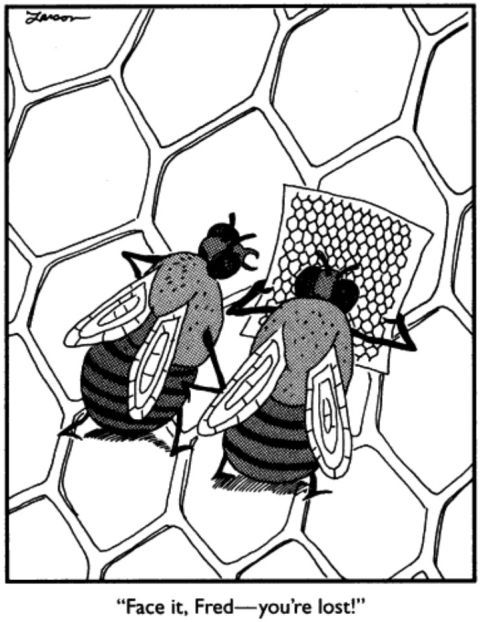
\includegraphics[height=\textwidth]{img/farside}
   \column{0.5\textwidth}
   \begin{itemize}
      \item \alert{common scenario:} you can recognize a good solution, but you don't know how to find one
      \item encountered by computer scientists (and everyone else, too)
      \item \alert{common approach:} try different options, evaluate outcomes to help choose next options to try
       \item this is called \alert{search}    
       \end{itemize}
   \end{columns}
\end{frame}

\begin{frame}{Evolutionary Algorithm: Vocabulary}

\begin{columns}
\begin{column}{0.25\textwidth}
\begin{itemize}
  \item individual
  \item population
  \item fitness
  \item genotype
  \item phenotype
  \item mutation
\end{itemize}
\end{column}
\begin{column}{0.75\textwidth}
\begin{figure}
    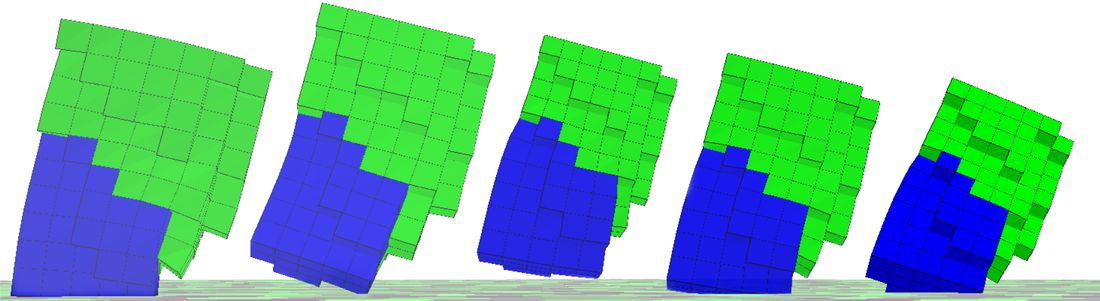
\includegraphics[width=\textwidth]{img/jumpertimeseries3_orig} \\
  \vspace{1ex}
  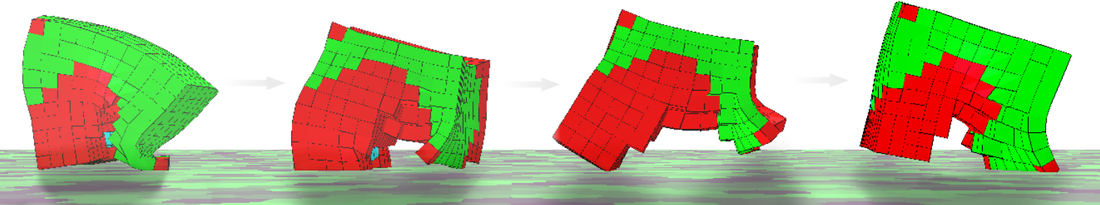
\includegraphics[width=\textwidth]{img/runnershortarrow_orig}
  \captionsetup{singlelinecheck=off,justification=raggedright}
  \caption{Illustrative examples of candidate solutions in an evolutionary algorithm \cite[Figures 1, 12]{Cheney2013UnshacklingEncoding}.}
\end{figure}
\end{column}
\end{columns}
    
\end{frame}

\begin{frame}{Evolutionary Algorithm: Overview}

\begin{figure}
  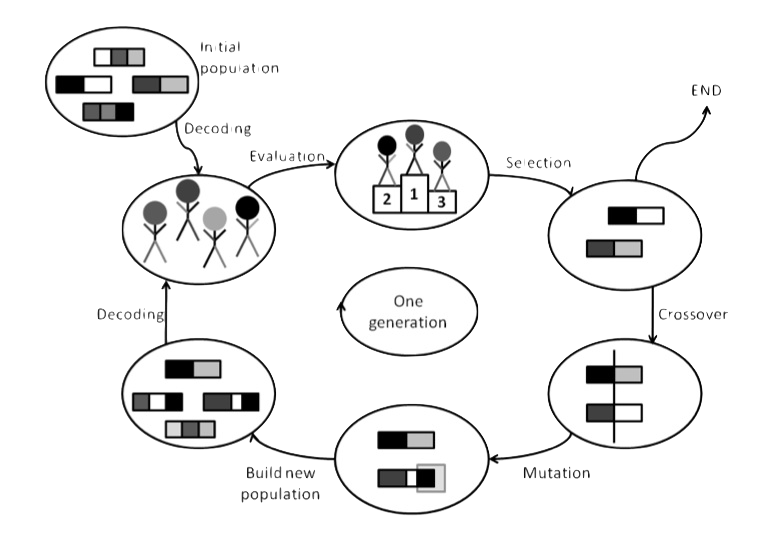
\includegraphics[width=0.8\textwidth]{img/working_principle_of_EA}
  \captionsetup{singlelinecheck=off,justification=raggedright}
  \caption{A schematic illustration of the evolutionary algorithm \cite[Figure 1]{Prothmann2009EvolutionaryOptimisation}.}
\end{figure}
    
\end{frame}


\begin{frame}{Evolutionary Algorithm: Example}
\begin{figure}
  \includemedia[width=\linewidth,height=0.6\textwidth, flashvars={scaleMode=zoom}]{}{http://www.youtube.com/v/z9ptOeByLA4?t=1m08s&amp;rel=0&amp;showinfo=0}
  \captionsetup{singlelinecheck=off,justification=raggedright}
\href{https://youtu.be/z9ptOeByLA4?t=1m08s}{\caption{Evolution in Action \cite{Cheney2013UnshacklingEncoding}}}
\end{figure}
\end{frame}

\begin{frame}{Evolutionary Algorithm: Problem Statement}
  
  \begin{columns}
\begin{column}{0.6\textwidth}
 What makes an evolutionary algorithm work?
\end{column}
\begin{column}{0.4\textwidth}
\begin{center}
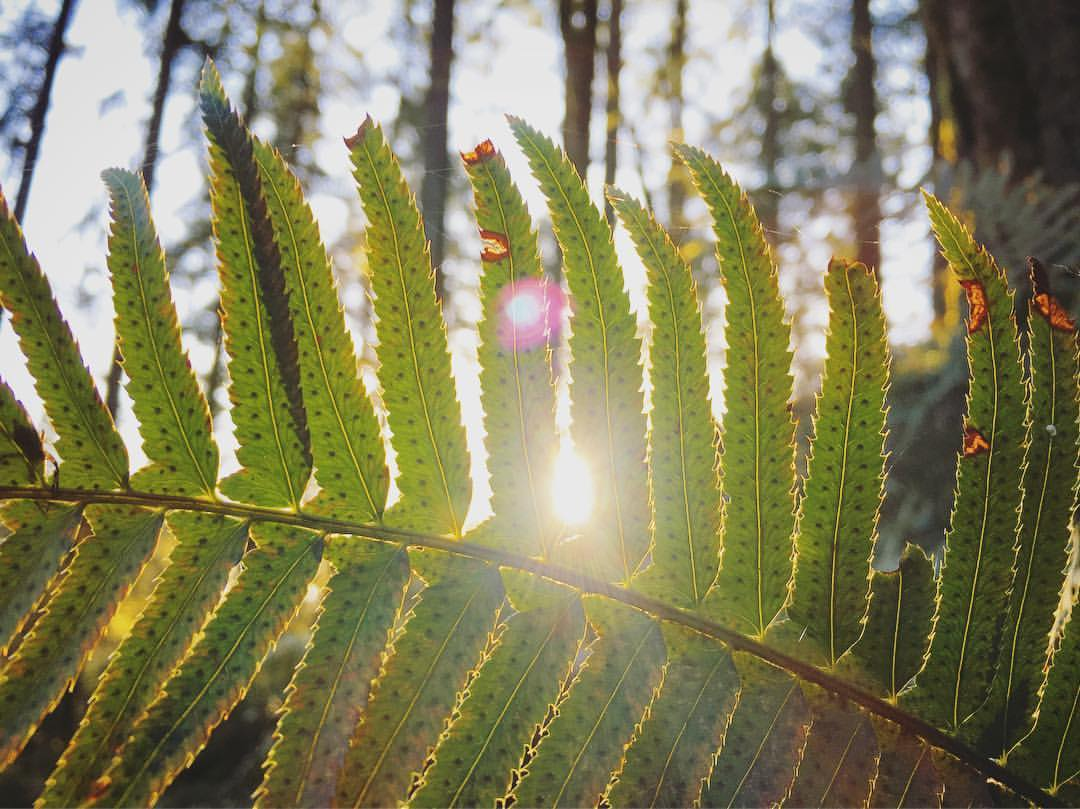
\includegraphics[width=\textwidth,trim={7cm 0 13cm 0},clip]{img/sunfern}
\end{center}
\end{column}
\end{columns}
 
\end{frame}

\section{Defining Evolvability}

\begin{frame}{Defining Evolvability}
consensus: the amount of \textcolor{h2}{useful} \textcolor{h1}{variation} generated by the evolutionary process
\begin{itemize}
  \item evolvability as the amount of \textcolor{h1}{\textbf{novel variation}} generated
  \item evolvability the proportion of variation that is \textcolor{h2}{\textbf{useful}}
\end{itemize}
\end{frame}

% \begin{frame}{The Evolvability Conundrum}
% How can natural selection ``favor properties hat may prove useful to a given lineage in the future, but have no present adaptive function''? \cite{Pigliucci2008IsEvolvable}
% \end{frame}


\subsection{Evolvability as Novel Variation}

\begin{frame}{Evolvability as Novel Variation}
	\begin{figure}
 \centering
    \begin{subfigure}[b]{0.5\textwidth}
        \centering
    	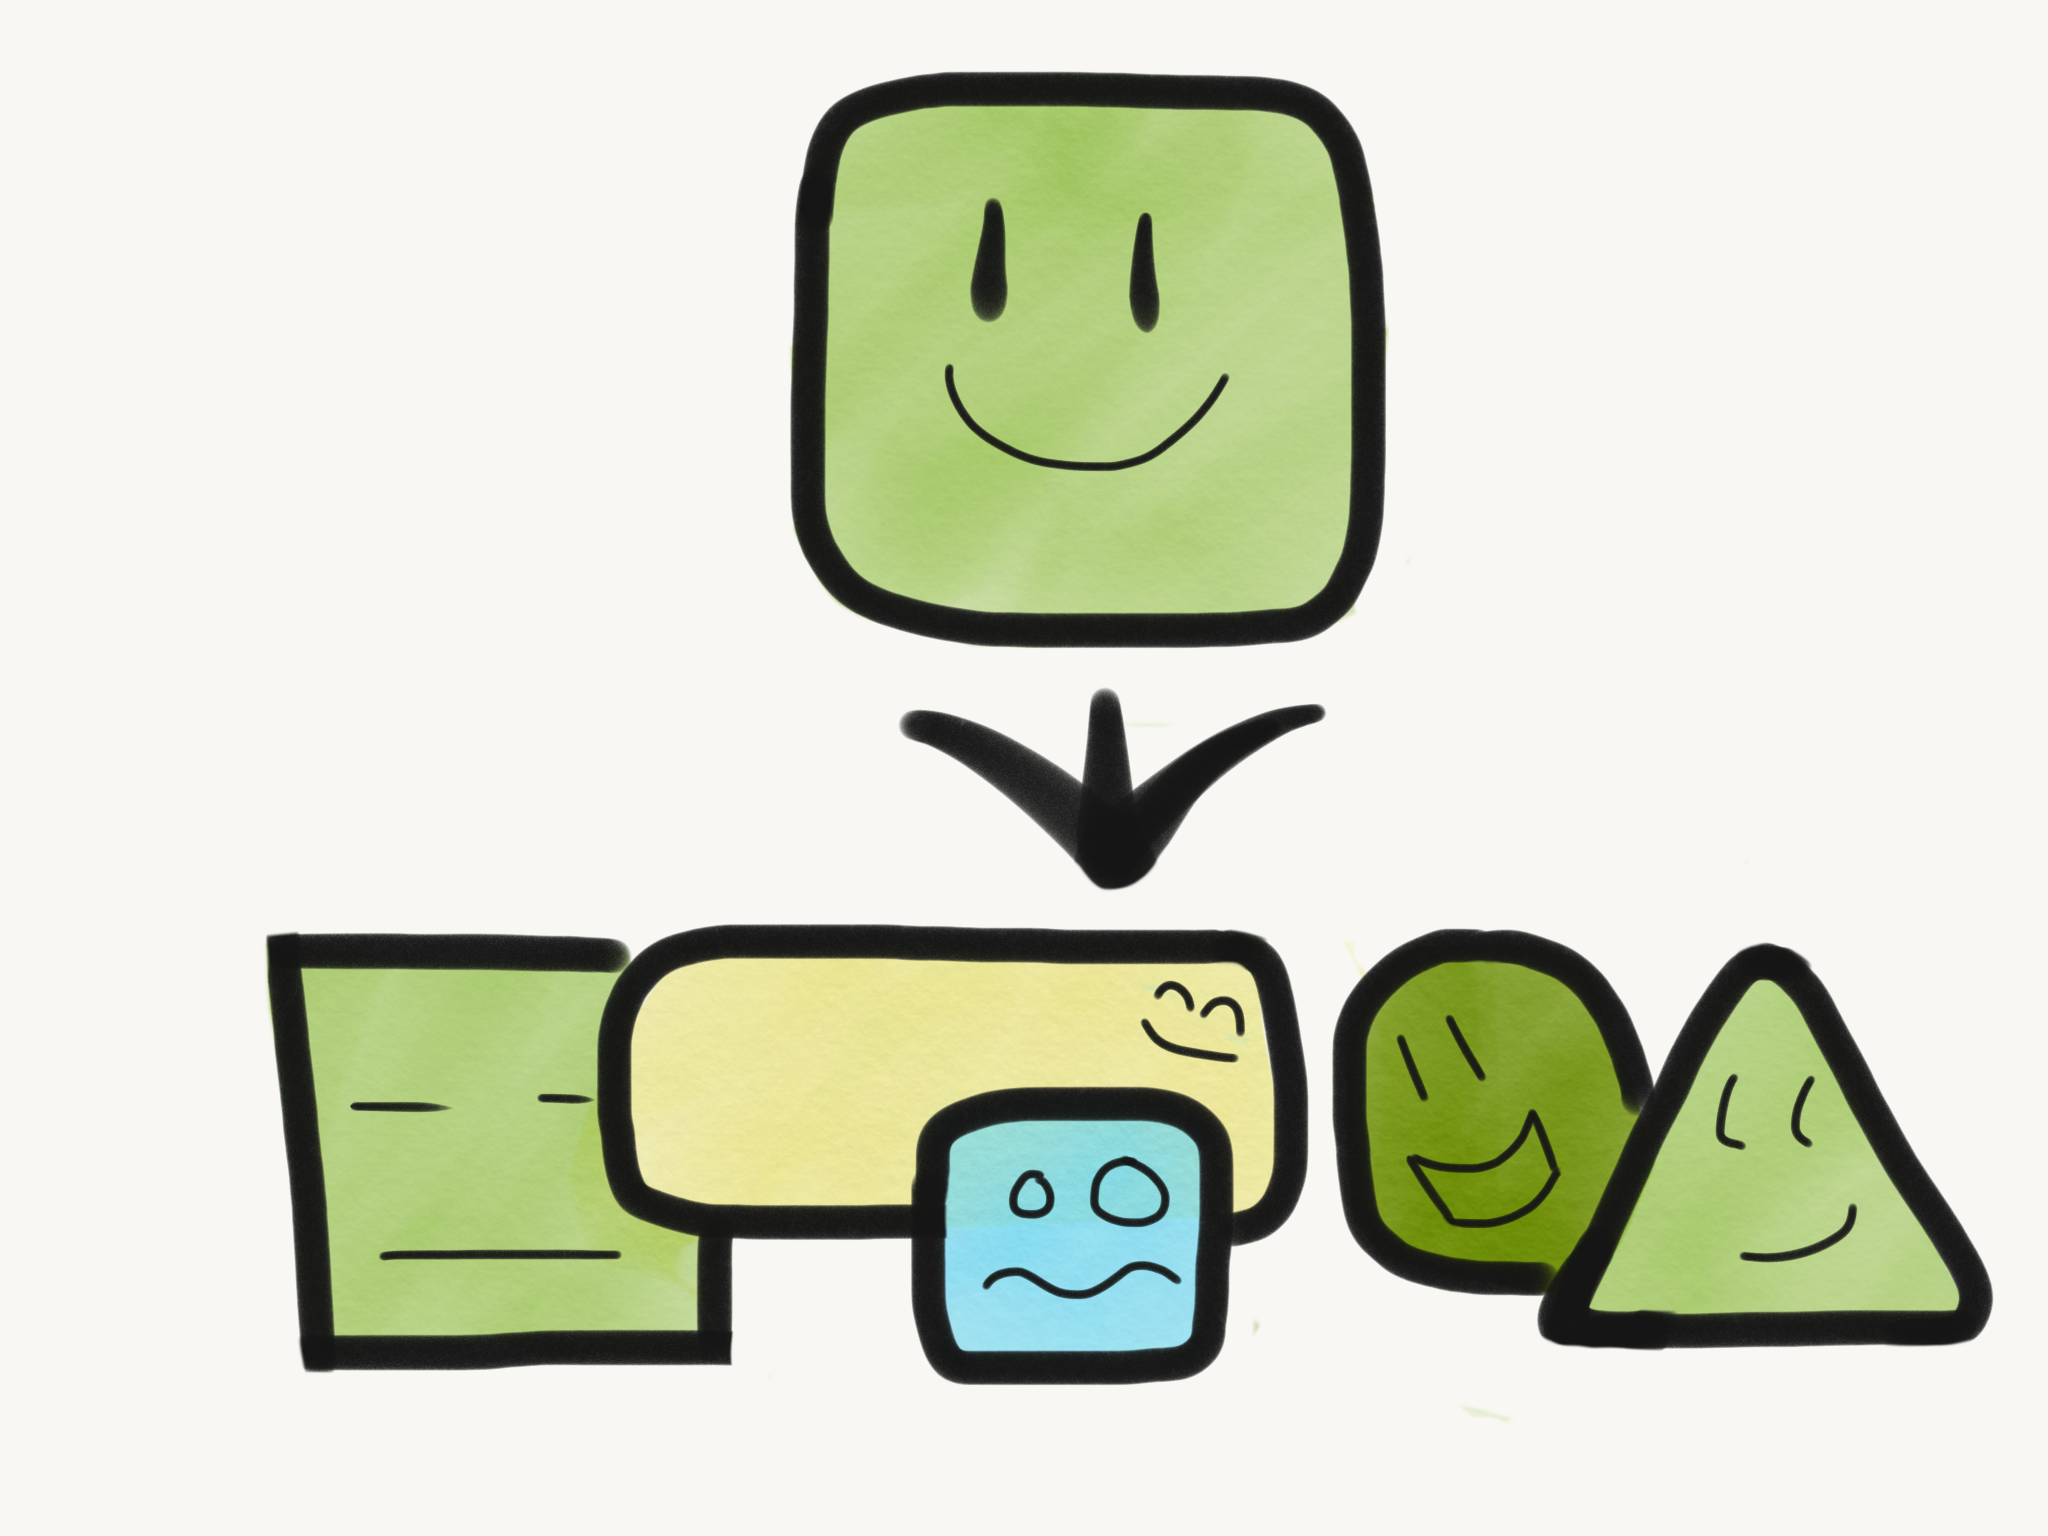
\includegraphics[width=\textwidth]{img/individual_evolvability.png}
        \caption{high individual evolvability}
        \label{subfig:canalization}
    \end{subfigure}%
    \hfill
    \begin{subfigure}[b]{0.5\textwidth}
        \centering
        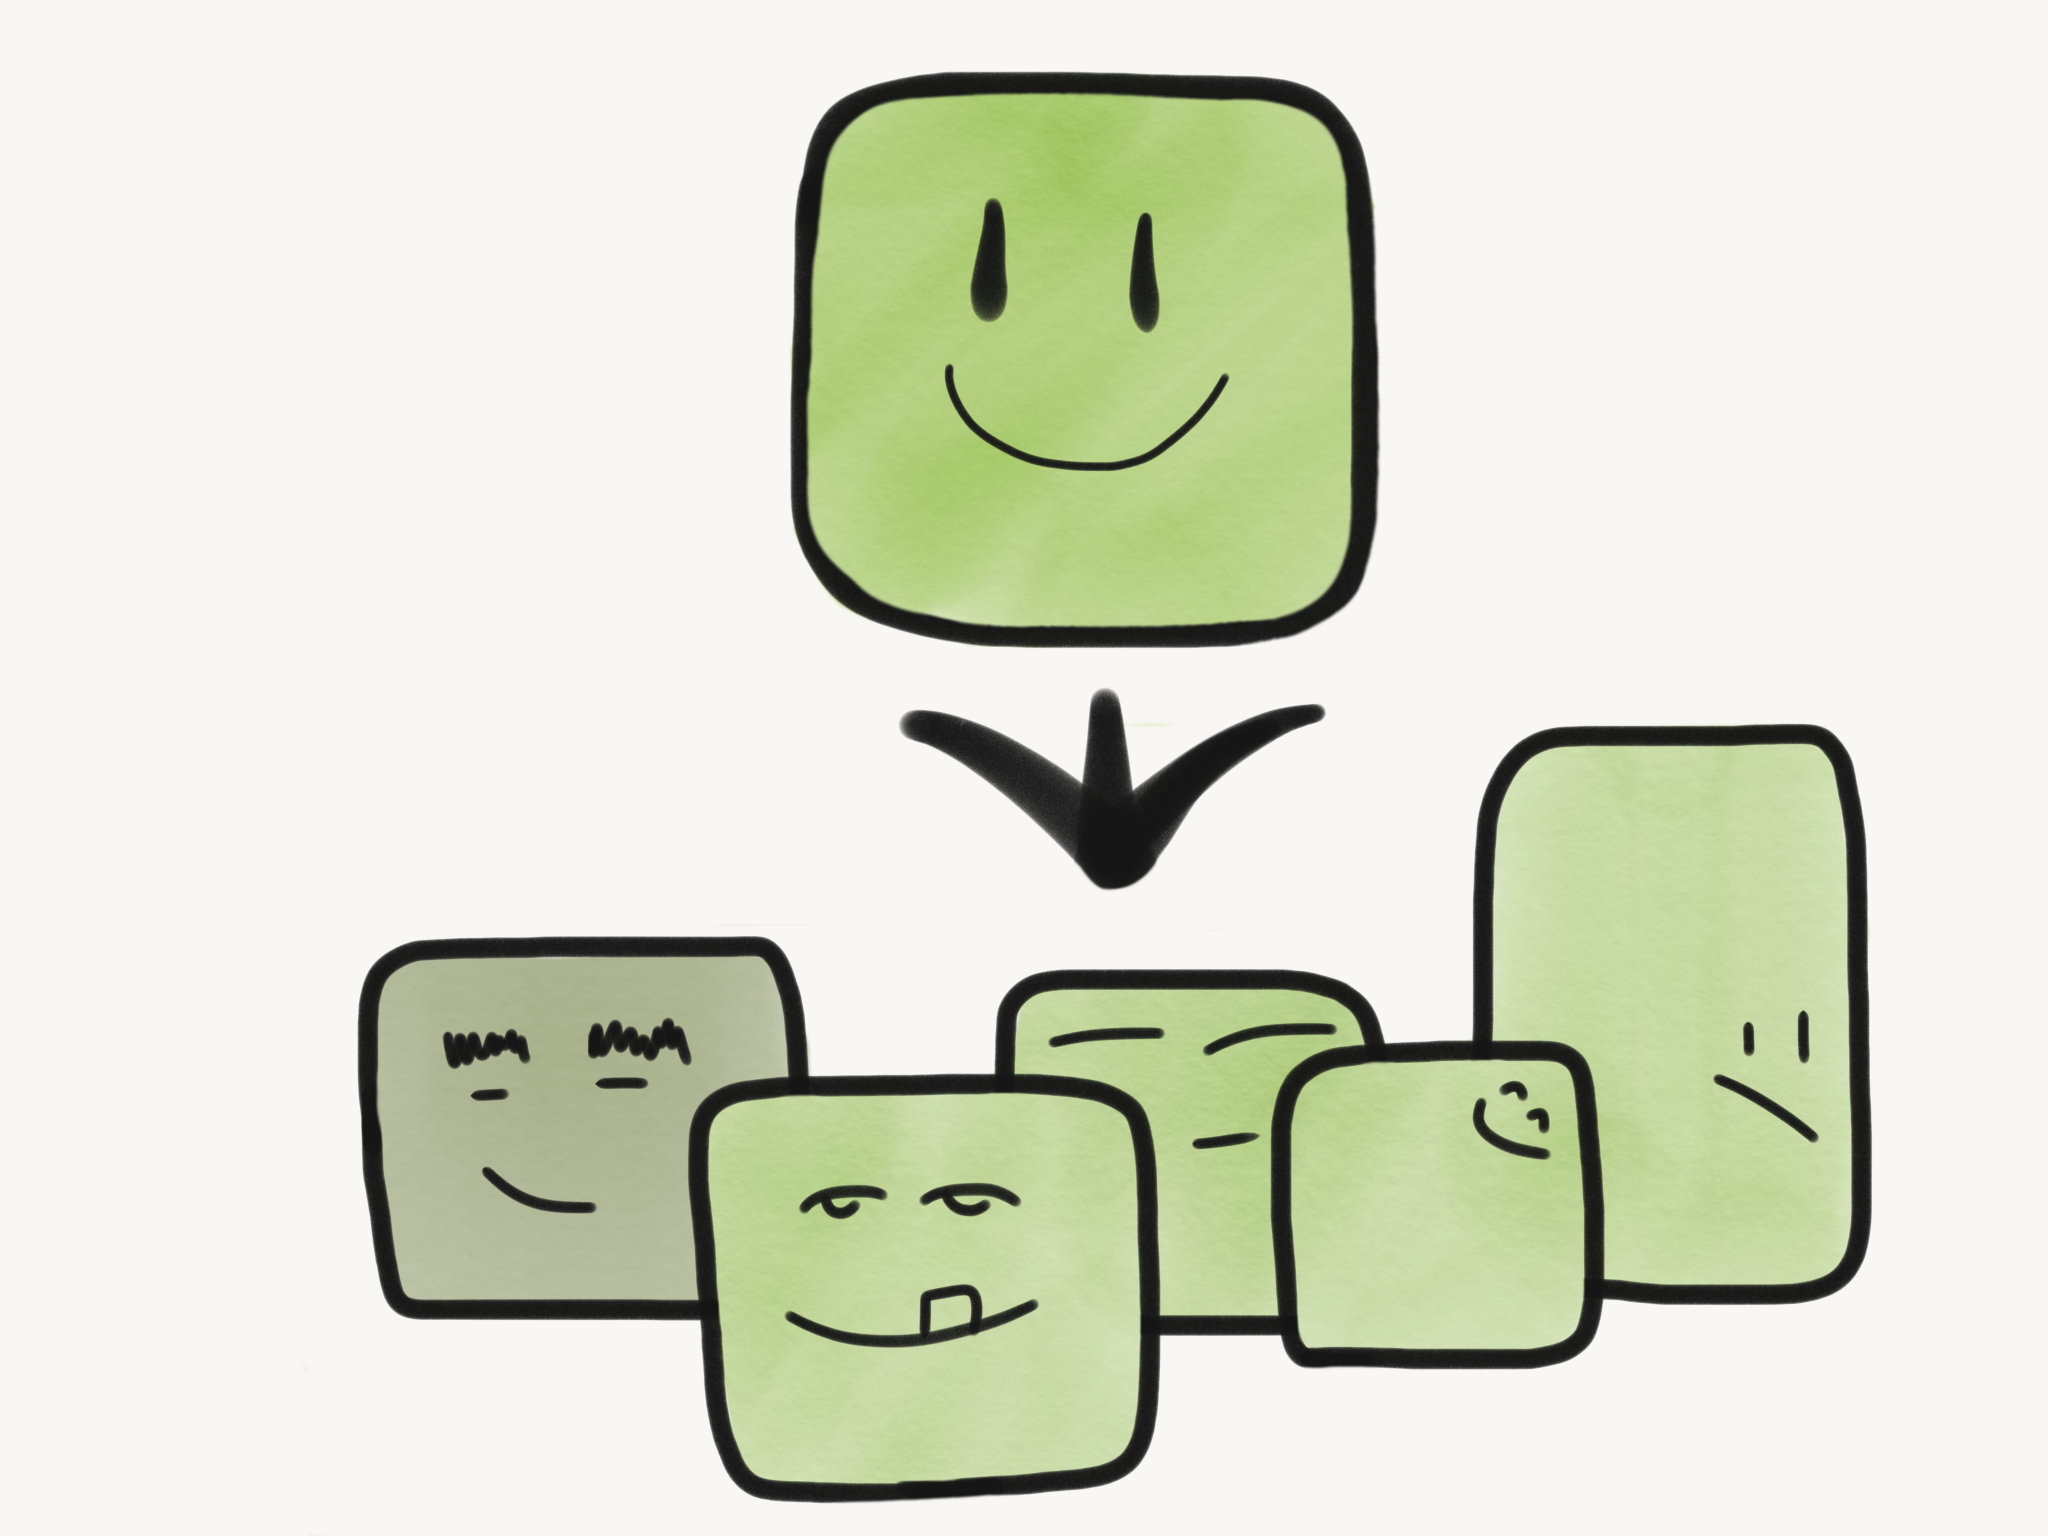
\includegraphics[width=\textwidth]{img/low_individual_evolvability.png}
        \caption{low individual evolvability}
        \label{subfig:no_canalization}
    \end{subfigure}
 	\captionsetup{singlelinecheck=off,justification=raggedright}
    \vspace{-4ex}
  \captionsetup{singlelinecheck=off,justification=raggedright}
  \caption{An illustration of individual evolvability, considering evolvability as heritable variation \cite{Wilder2015ReconcilingEvolvability}.}
  \label{fig:high_vs_low_individual_evolvability}
\end{figure}
\end{frame}

\subsection{Evolvability as Bias towards Useful Variation}

\begin{frame}{Evolvability as Bias towards Useful Variation}
  \begin{figure}
    \centering
    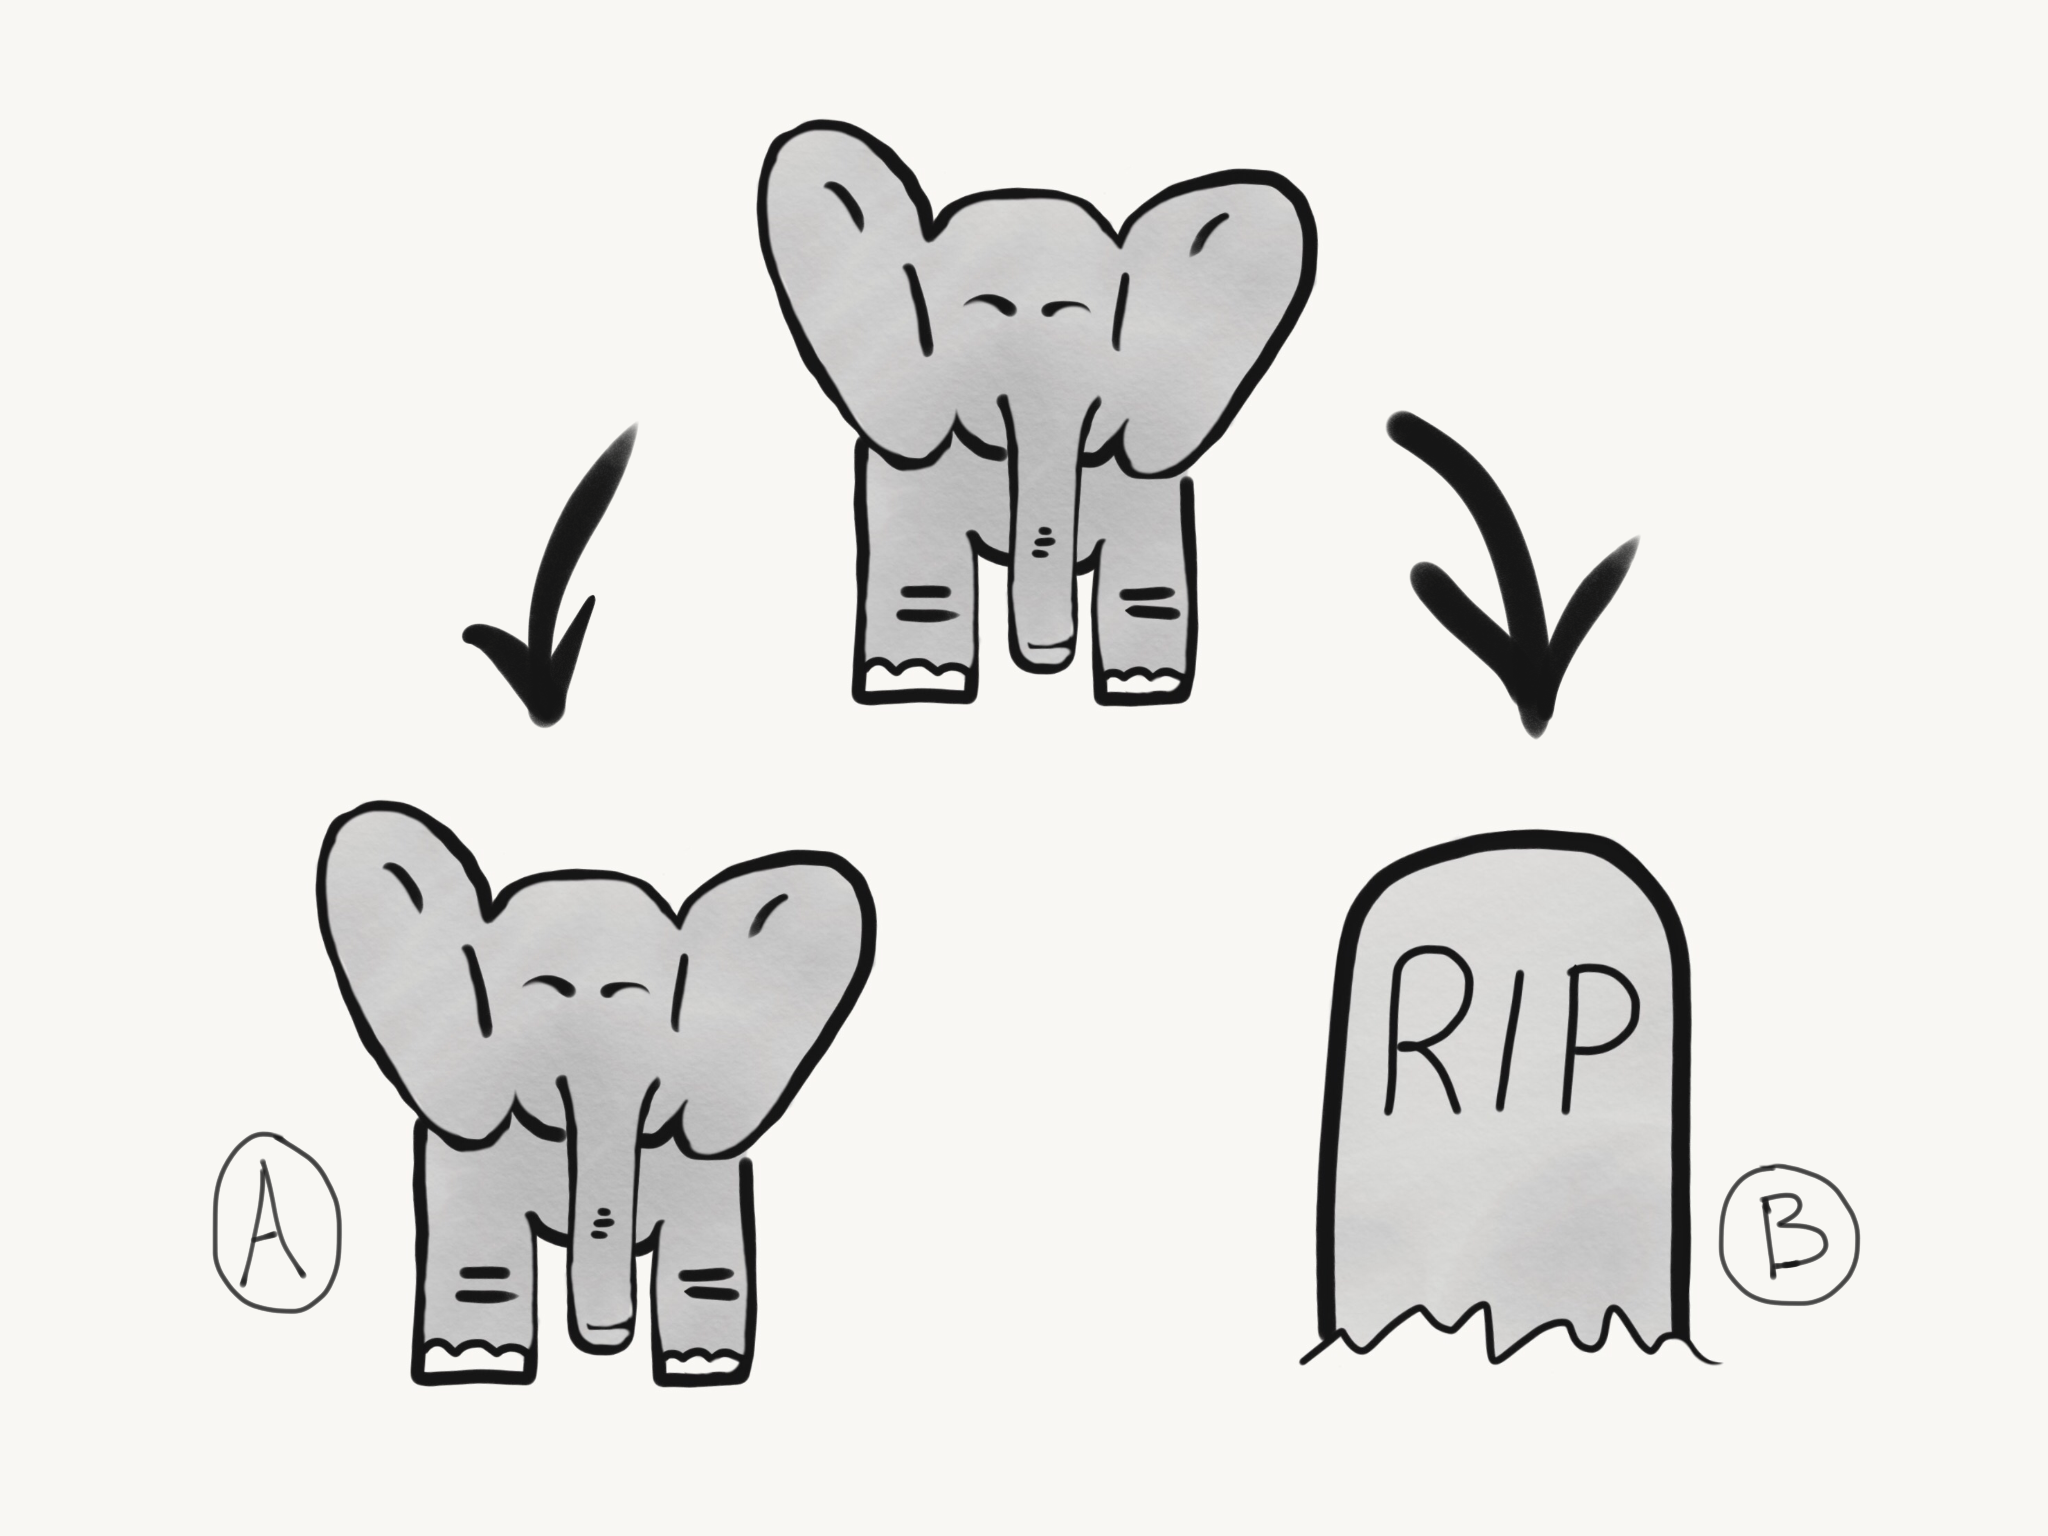
\includegraphics[width=0.8\textwidth]{img/robustness}
 	\captionsetup{singlelinecheck=off,justification=raggedright}
  	\caption{Illustration of robustness; high evolvability left and low evolvability right \cite{Downing2015IntelligenceSystems}.}
    \label{fig:robustness}
\end{figure}
\end{frame}

\begin{frame}{Evolvability as Bias towards Useful Variation}
  \begin{figure}
    \centering
    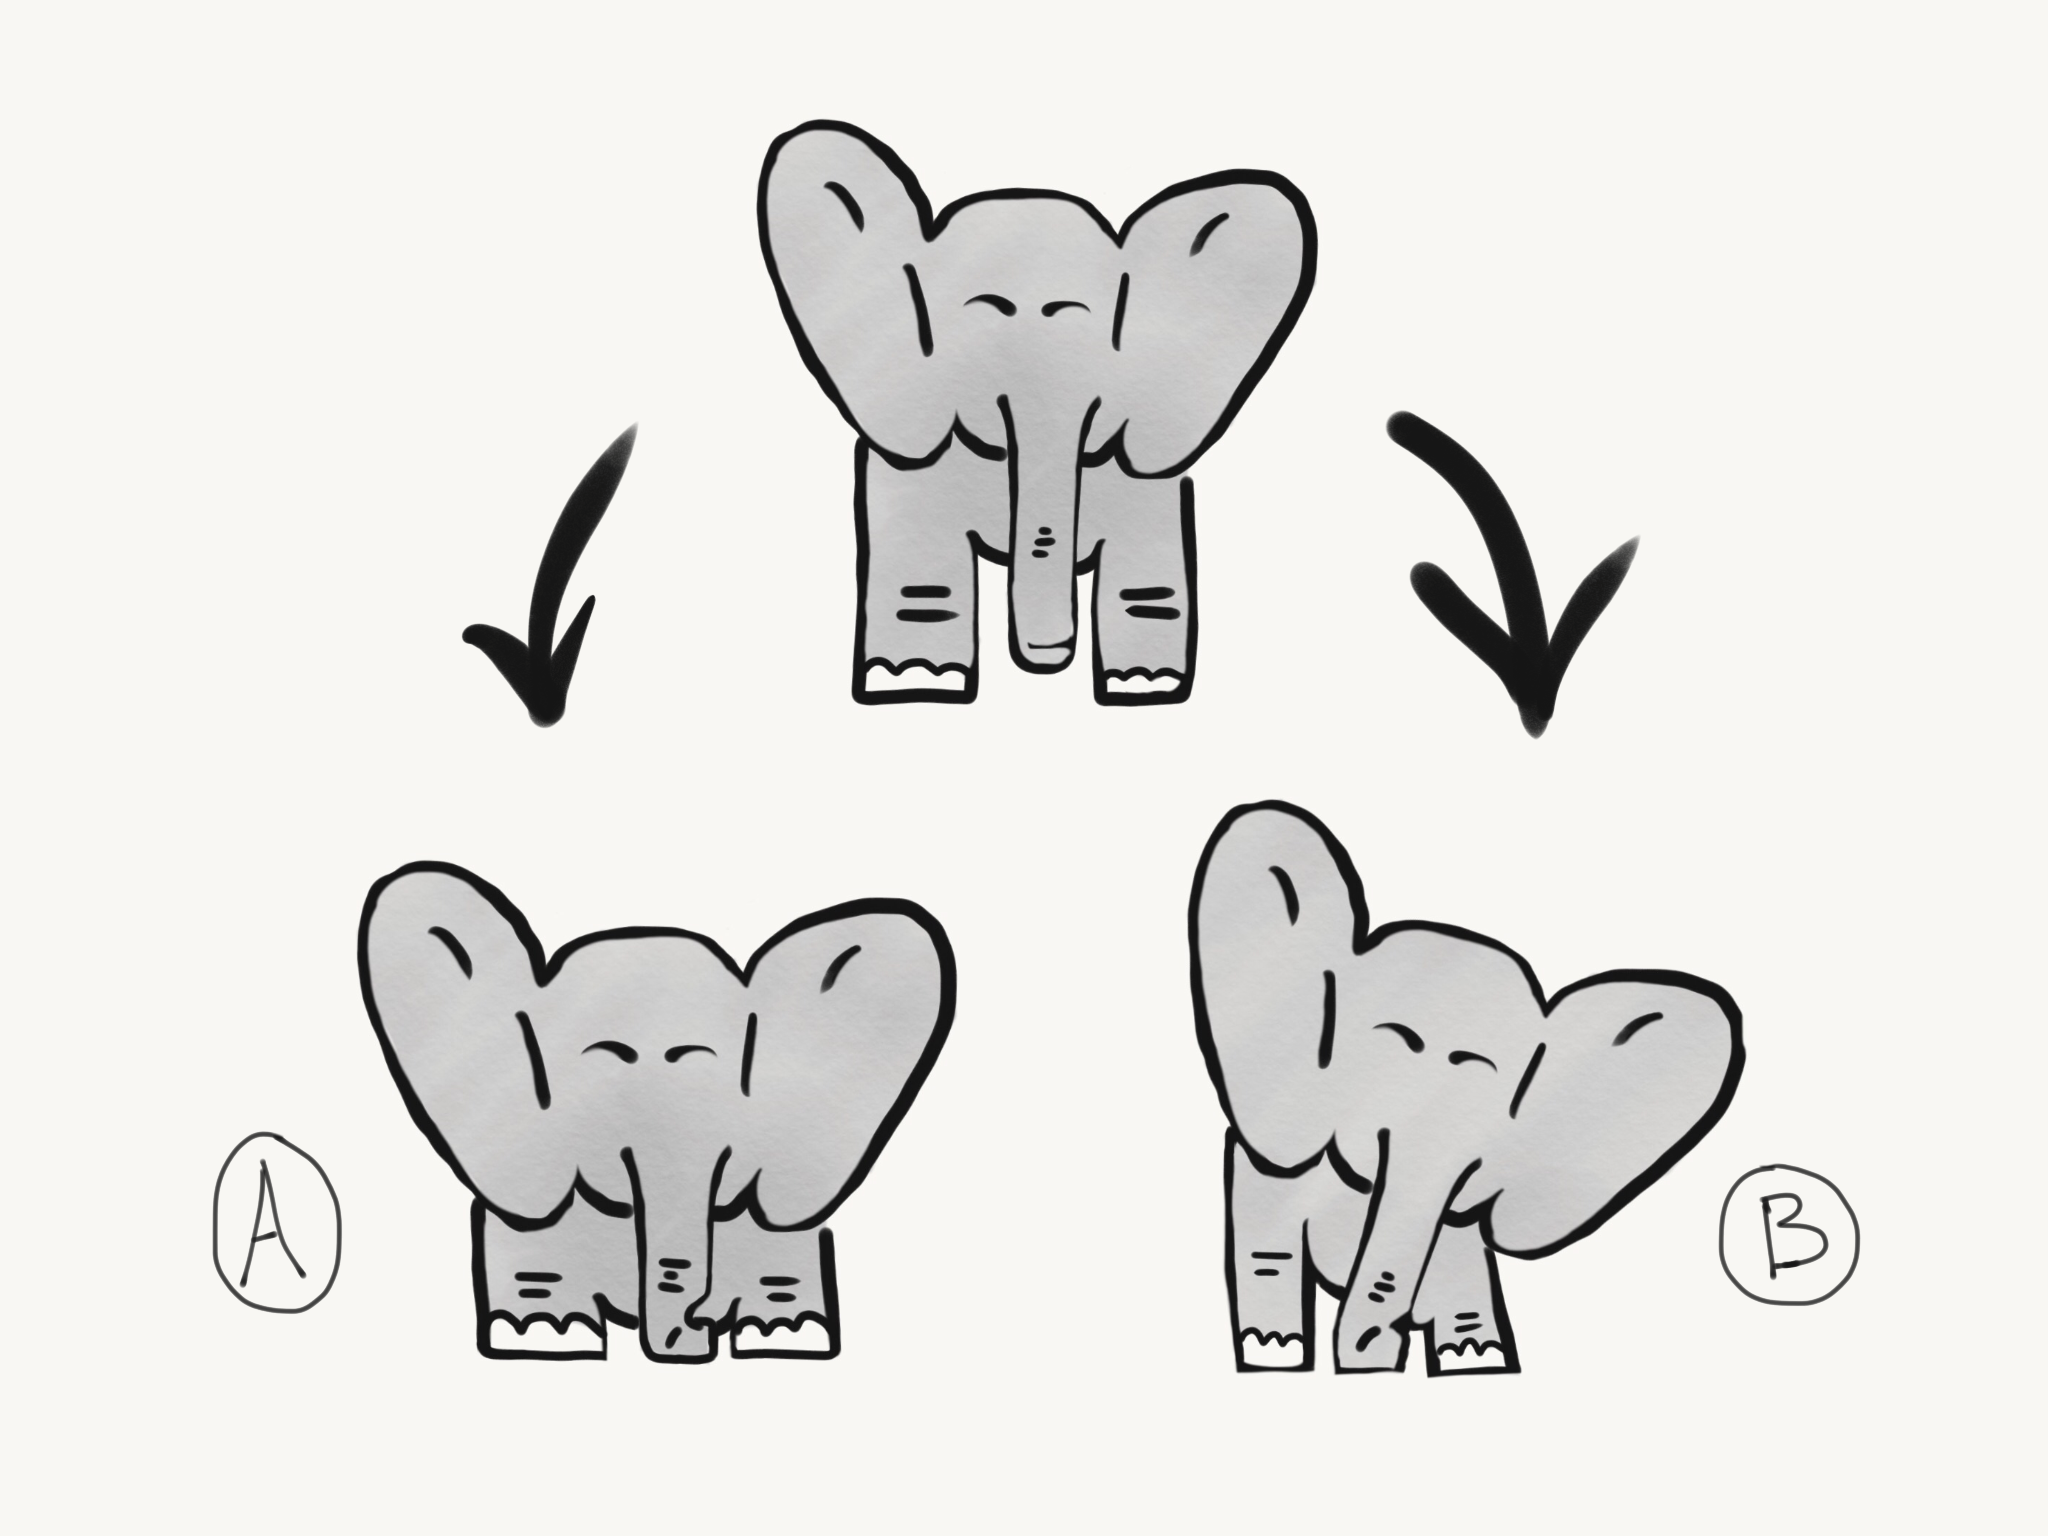
\includegraphics[width=0.8\textwidth]{img/developmental_constraint}
 	\captionsetup{singlelinecheck=off,justification=raggedright}
  	\caption{Illustration of developmental constraint; high evolvability left and low evolvability right \cite{Smith1985DevelopmentalBiology,Tuinstra1990LackDevelopment}.}
    \label{fig:developmental_constraint}
\end{figure}
\end{frame}

\subsection{Visualizing Evolvability}

\begin{frame}{Generating and Reading an Evolvability Signature}
  \begin{figure}
  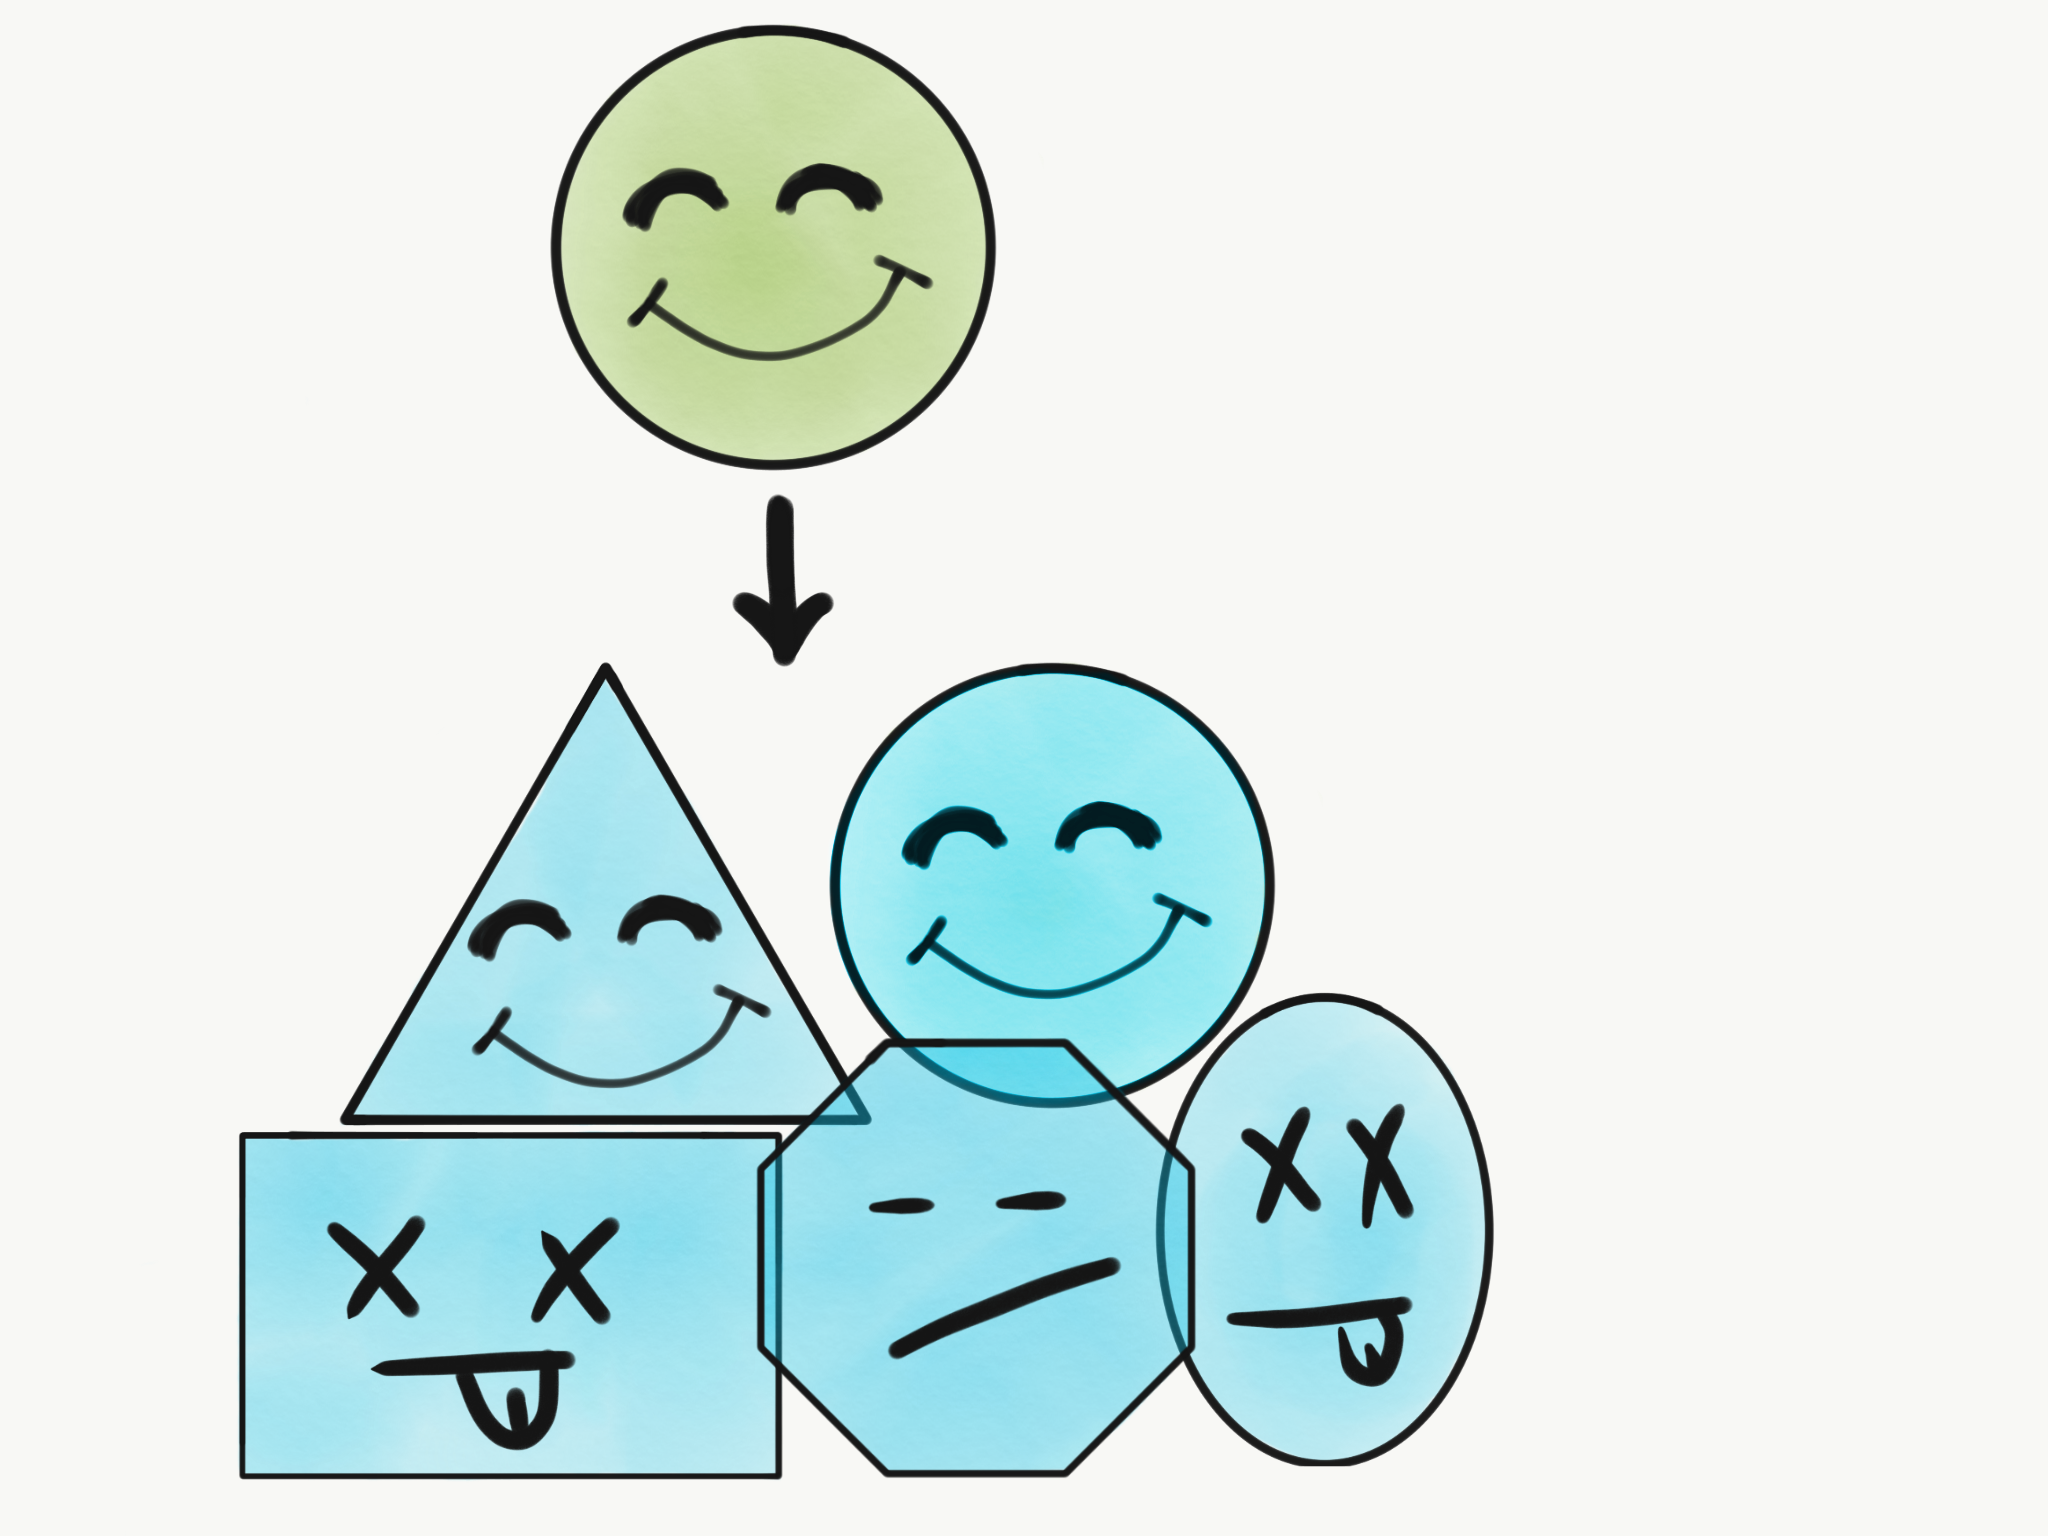
\includegraphics[width=0.5\textwidth]{img/evol_sig_gen}
  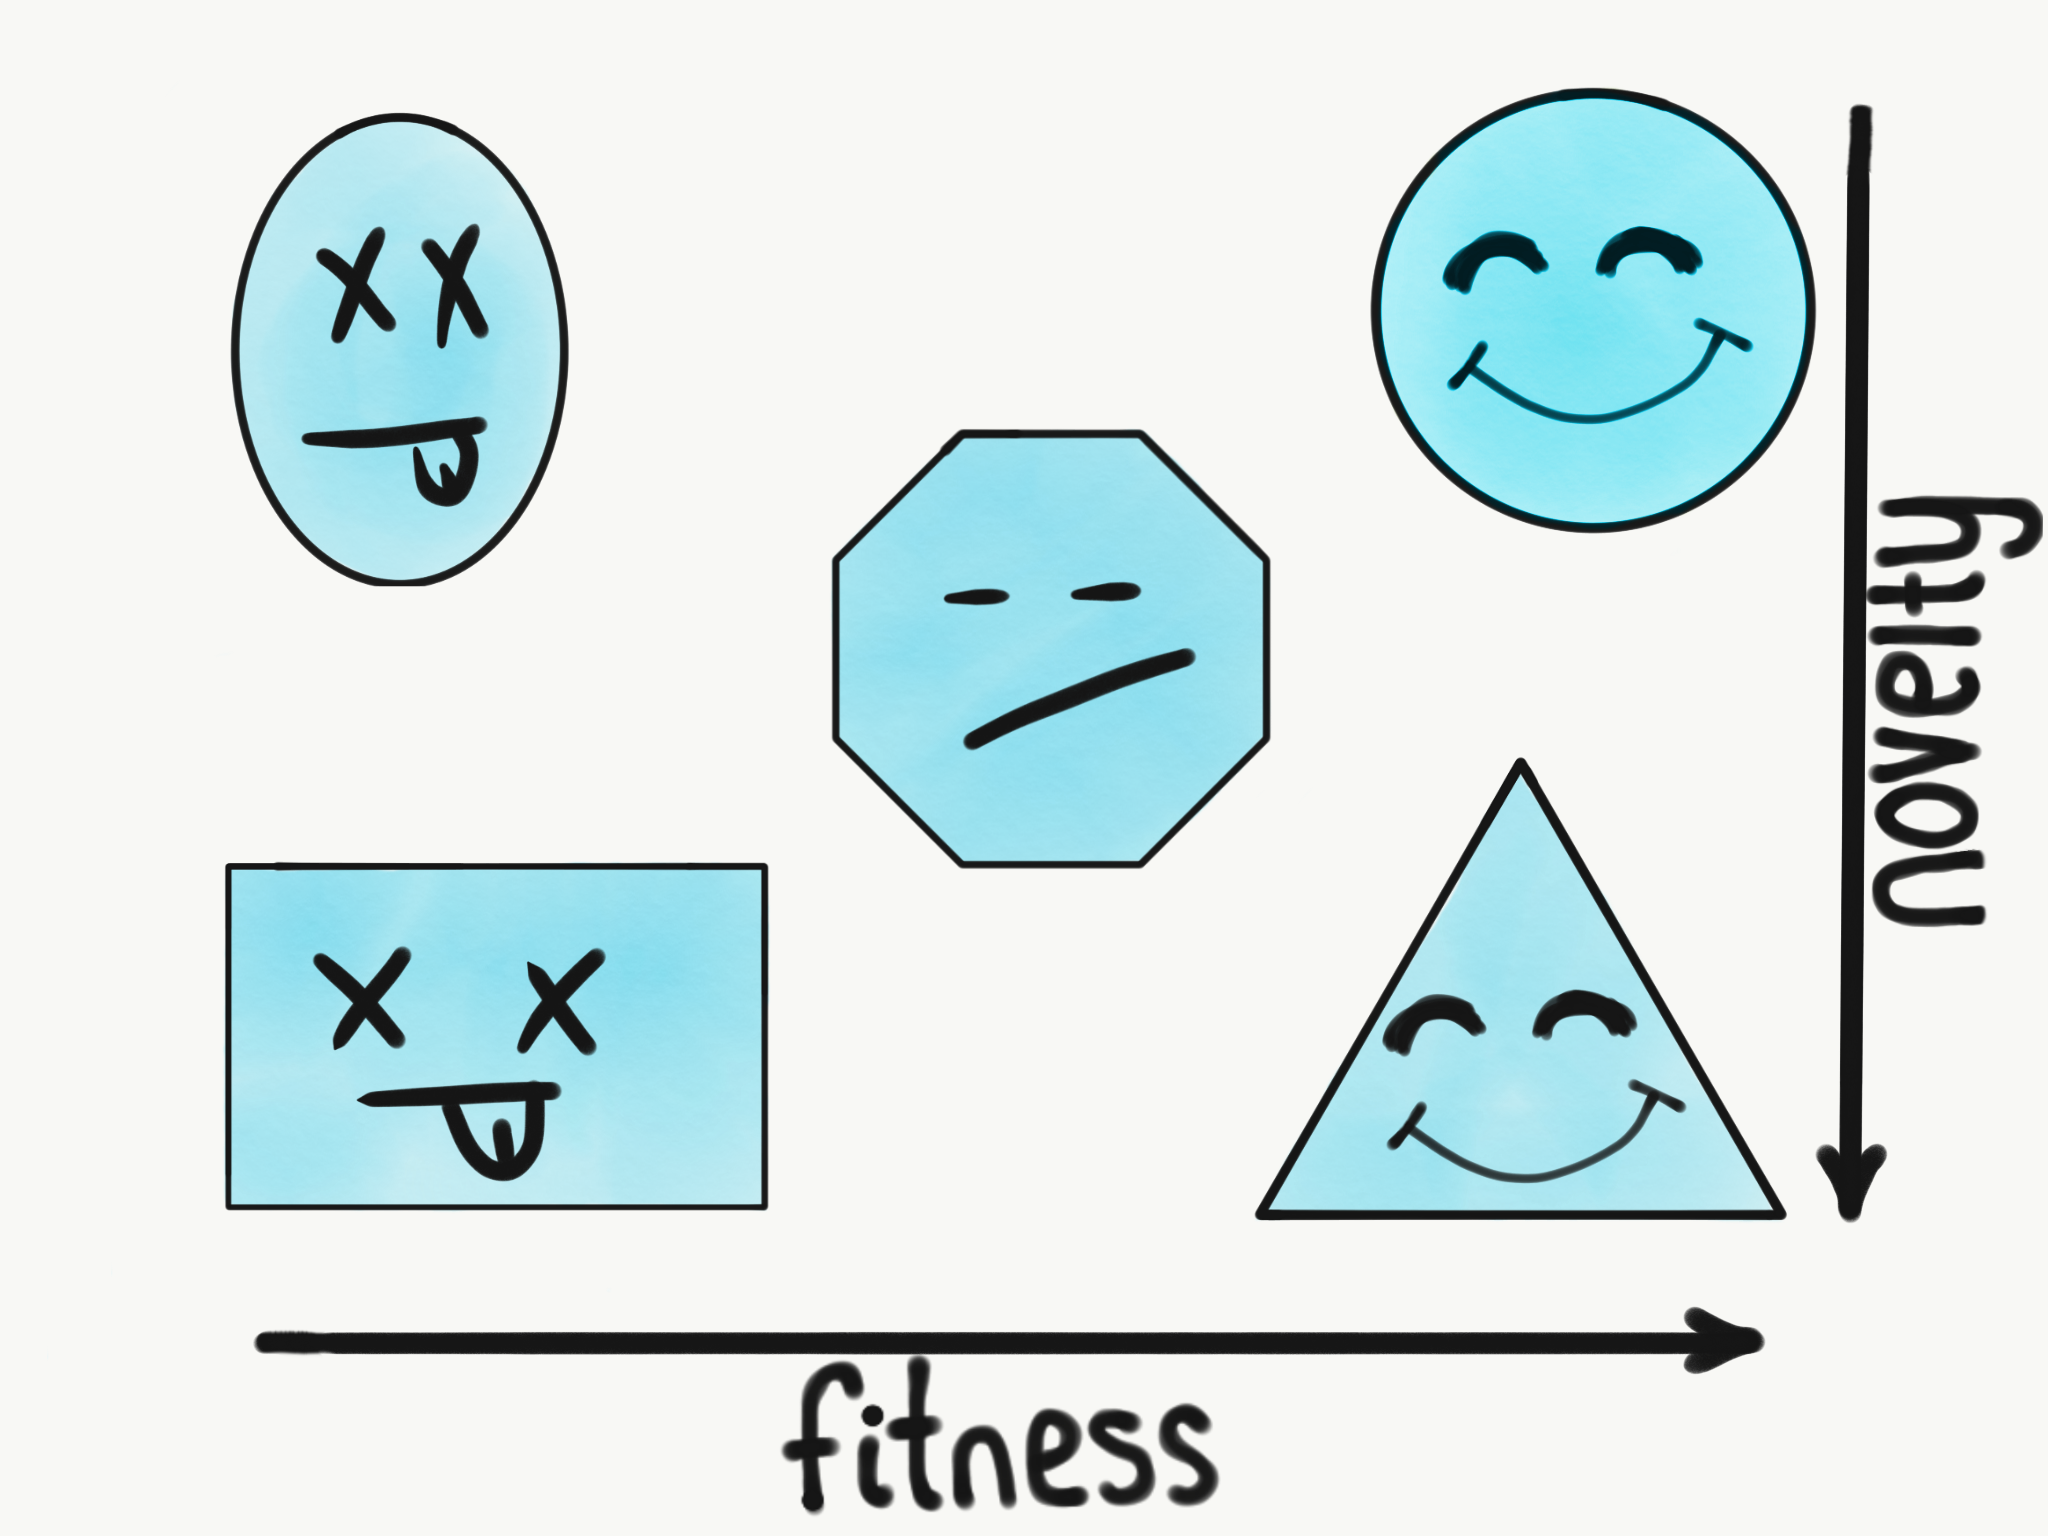
\includegraphics[width=0.5\textwidth]{img/evol_sig_read}
  \captionsetup{singlelinecheck=off,justification=raggedright}
  \caption{Cartoon illustration describing the creation and layout of an evolvability signature diagram \cite{Tarapore2015EvolvabilityBenchmarks}.}
  \label{fig:reading_evolvability_signature}
\end{figure}
\end{frame}



\section{Causes of Evolvability: Intuition}

\begin{frame}{Summary}
  \alert{big idea}: internal system configuration determines the outcomes of change to the system
\end{frame}


\begin{frame}{Computer Science Intuition: Spaghetti Code}
  idea: software without compartmentalization, error handling, with hard-coded constants, etc. is much more difficult to alter in useful ways
  \begin{figure}
  \centering
  \begin{subfigure}[b]{0.5\textwidth}
    \centering
    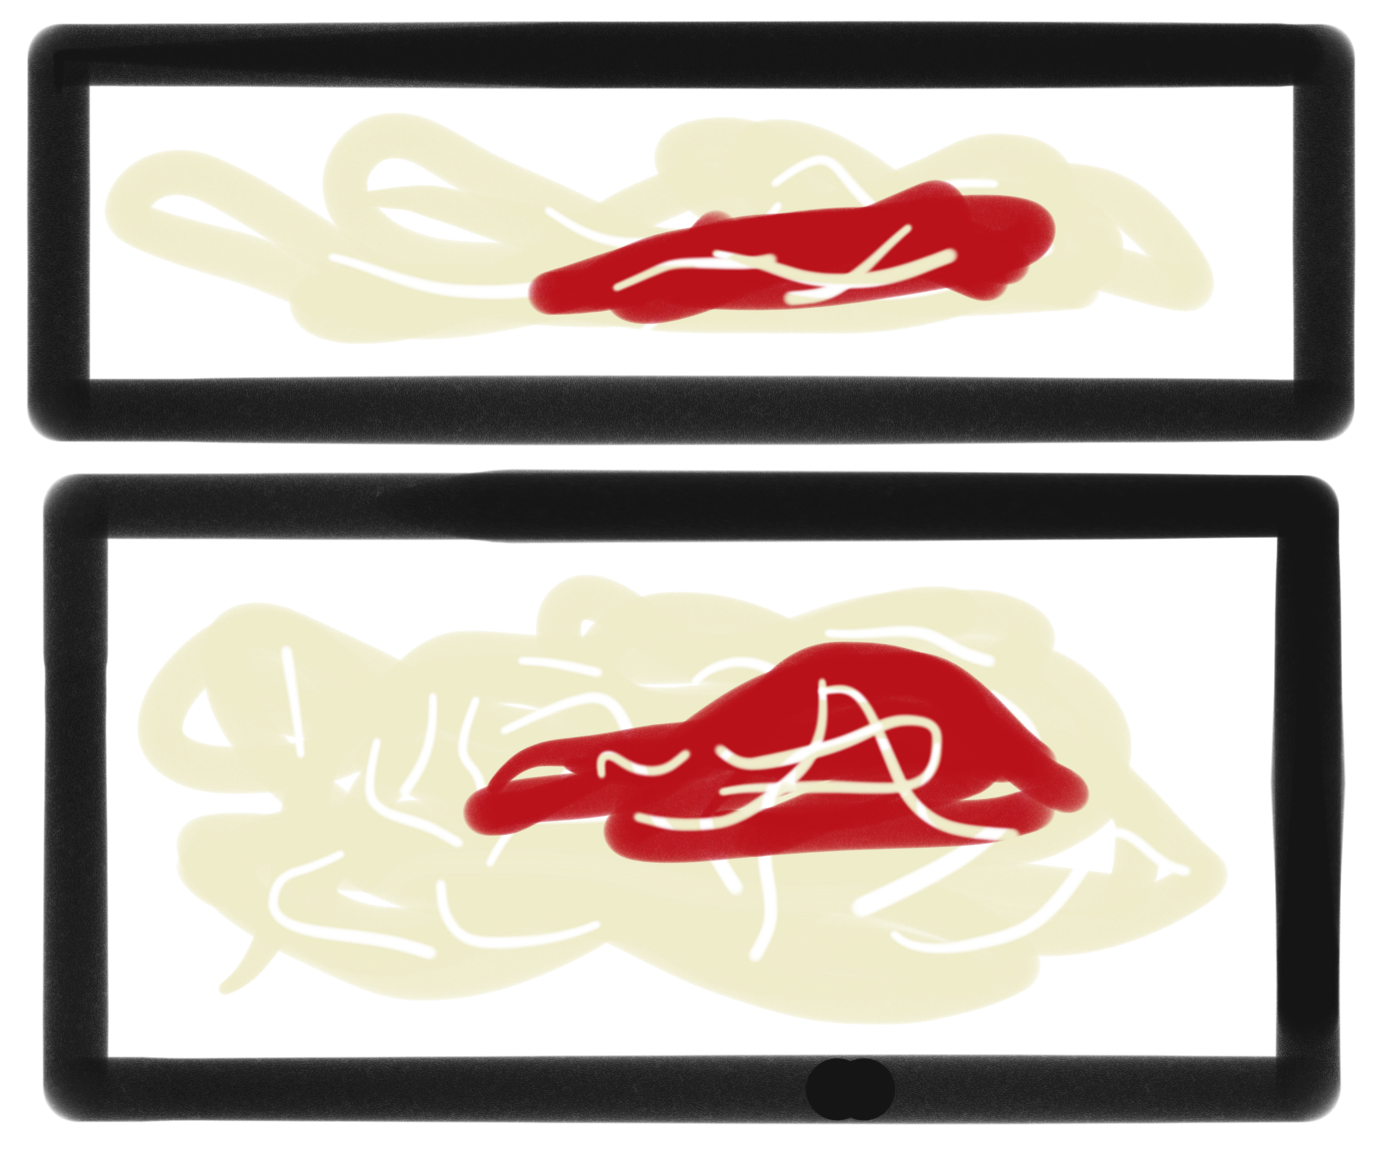
\includegraphics[width=\textwidth]{img/spaghetticode}
    \caption{spaghetti code}
    \label{subfig:spaghetti_code}
  \end{subfigure}%
  \hfill
  \begin{subfigure}[b]{0.5\textwidth}
    \centering
    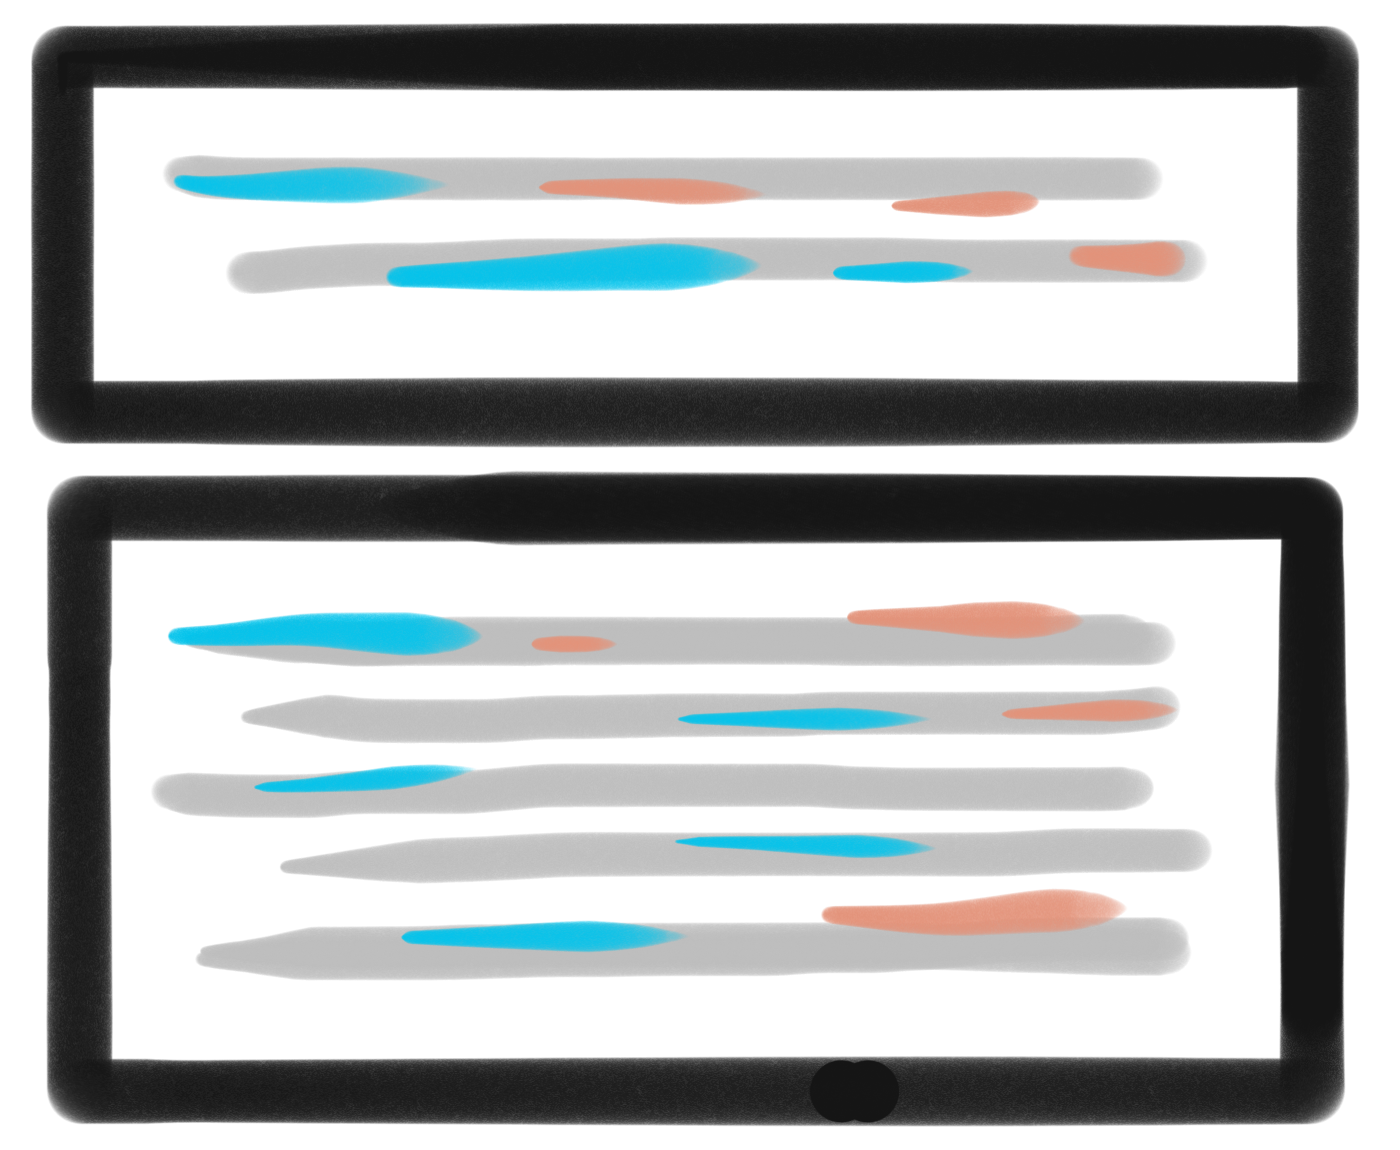
\includegraphics[width=\textwidth]{img/regularcode}
    \caption{regular code}
     \label{subfig:regular_code}
  \end{subfigure}
  \captionsetup{singlelinecheck=off,justification=raggedright}
  \caption{A cartoon comparison of spaghetti and regular code.}
  \label{fig:direct_irregular_vs_indirect_regular}
\end{figure}
\end{frame}

\begin{frame}{Computer Science Intuition: Spaghetti Code}
  idea: software without compartmentalization, error handling, with hard-coded constants, etc. is much more difficult to alter in useful ways
  \begin{figure}
  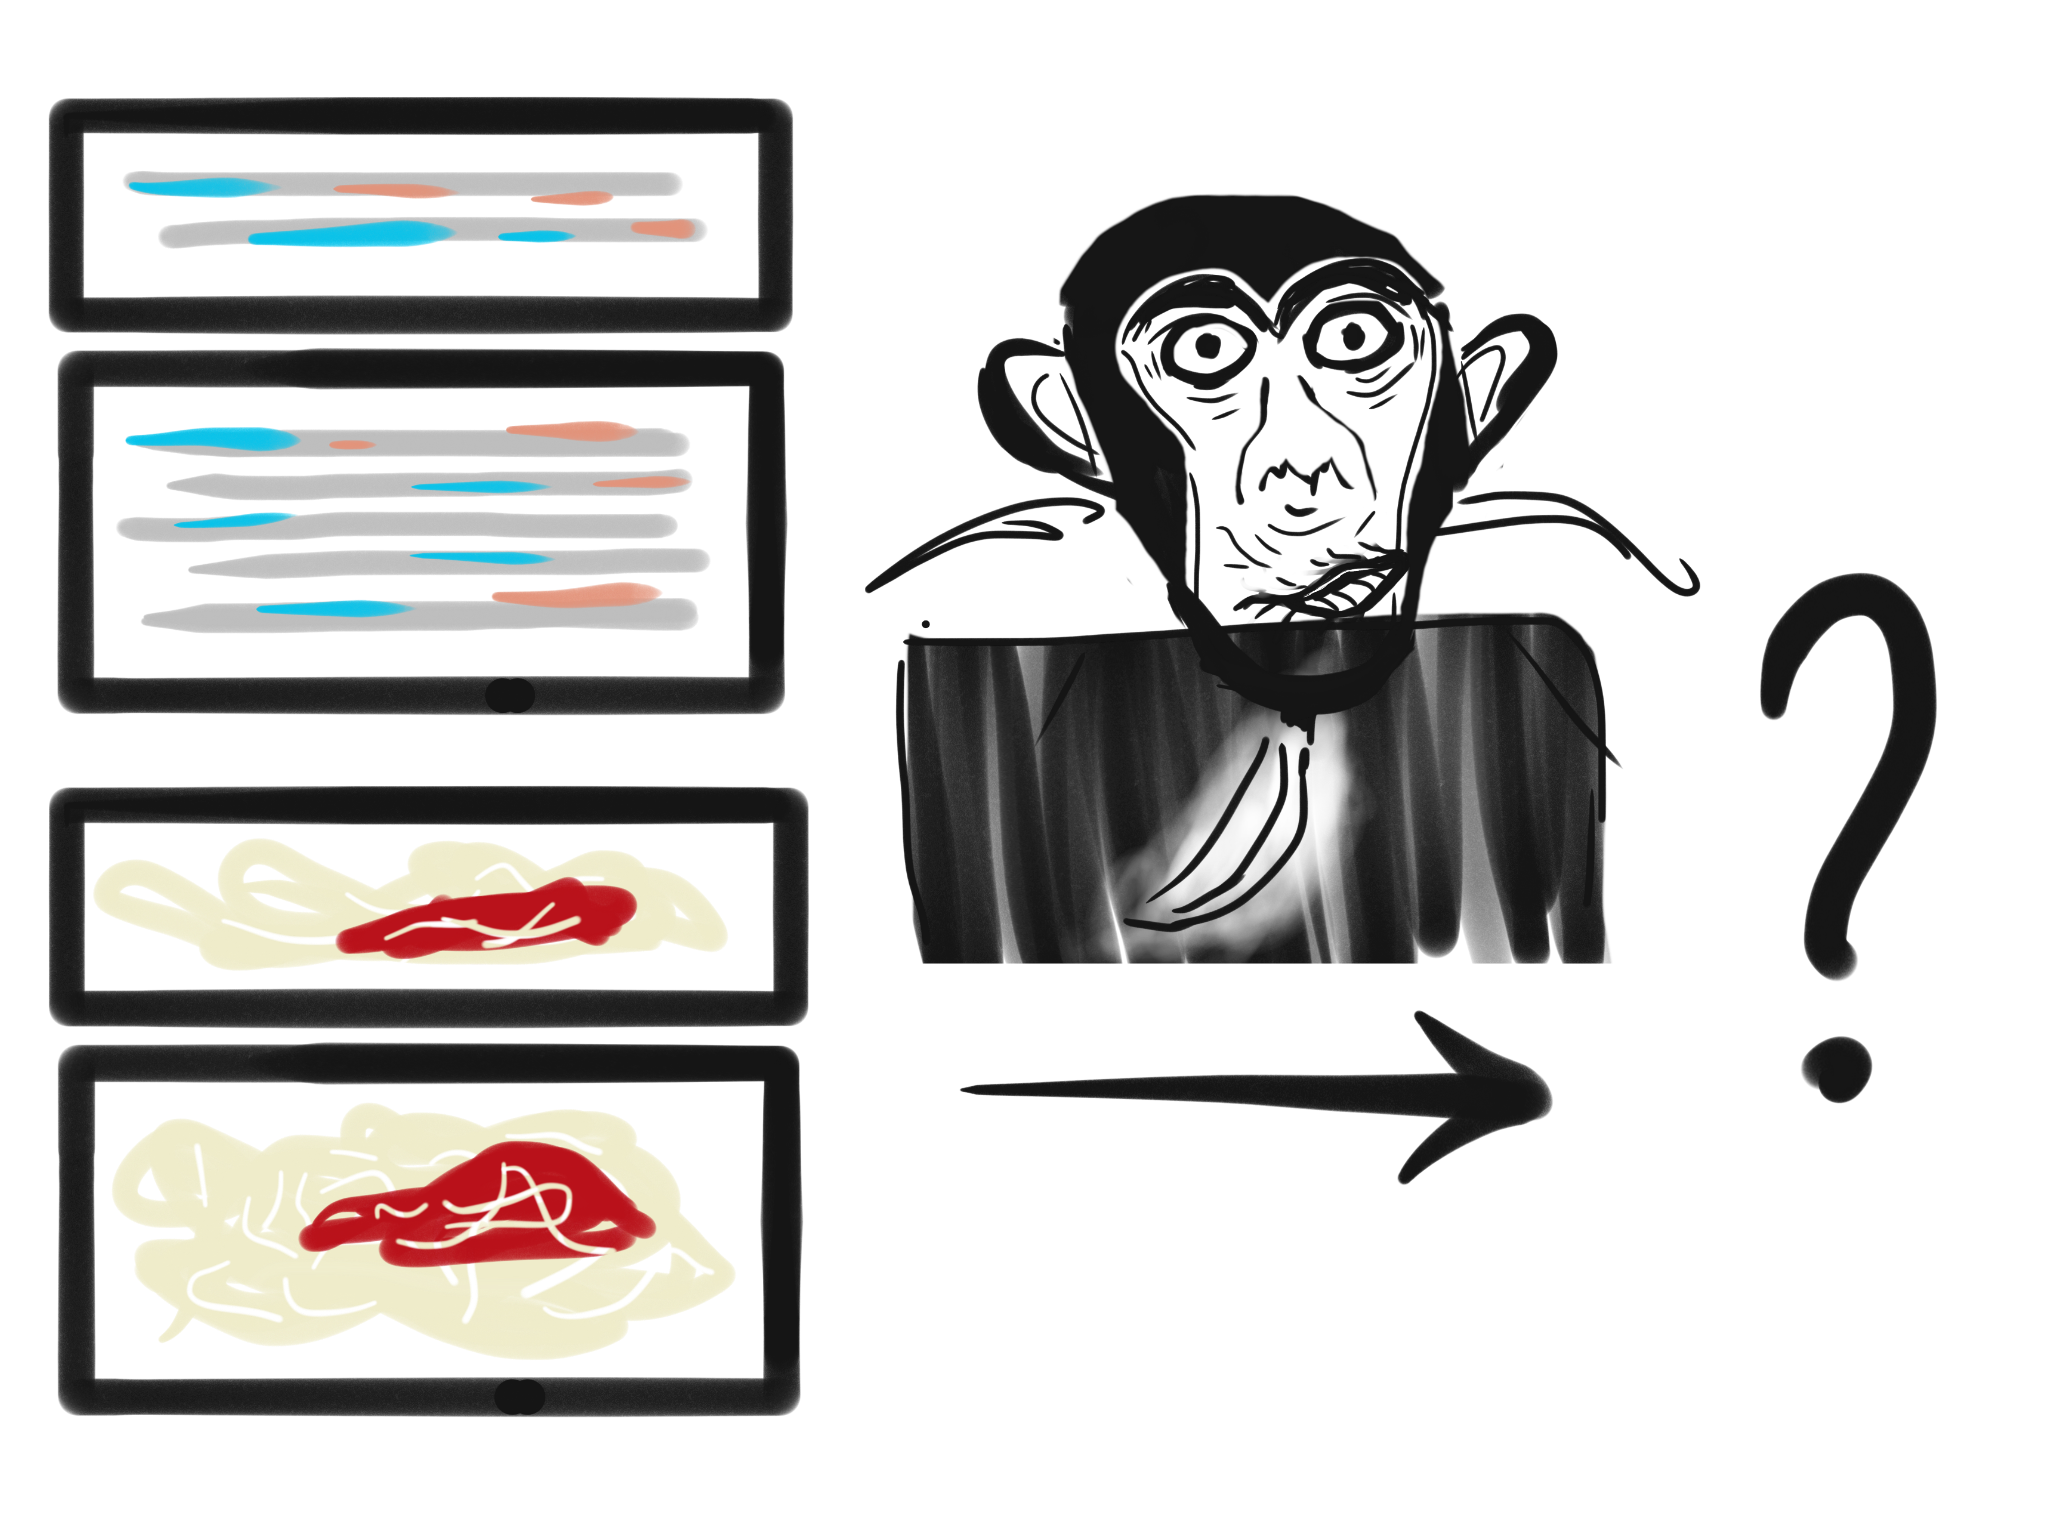
\includegraphics[width=0.6\textwidth]{img/spaghetti_monkey}
  \captionsetup{singlelinecheck=off,justification=raggedright}
  \caption{Spaghetti code and proper code might experience different distributions of outcomes from arbitrary changes to the software made by a junior developer from the local primate house.}
\end{figure}
\end{frame}

\begin{frame}{Biological Perspective: Intraindividual Degeneracy}
  idea: employing a diverse collection of substructures that provide identical or near-identical functionality promote robustness through redundancy while providing many jumping off points for variation through repurposing or elaboration
  \begin{figure}
 \begin{columns}
 \begin{column}{0.6\textwidth}
 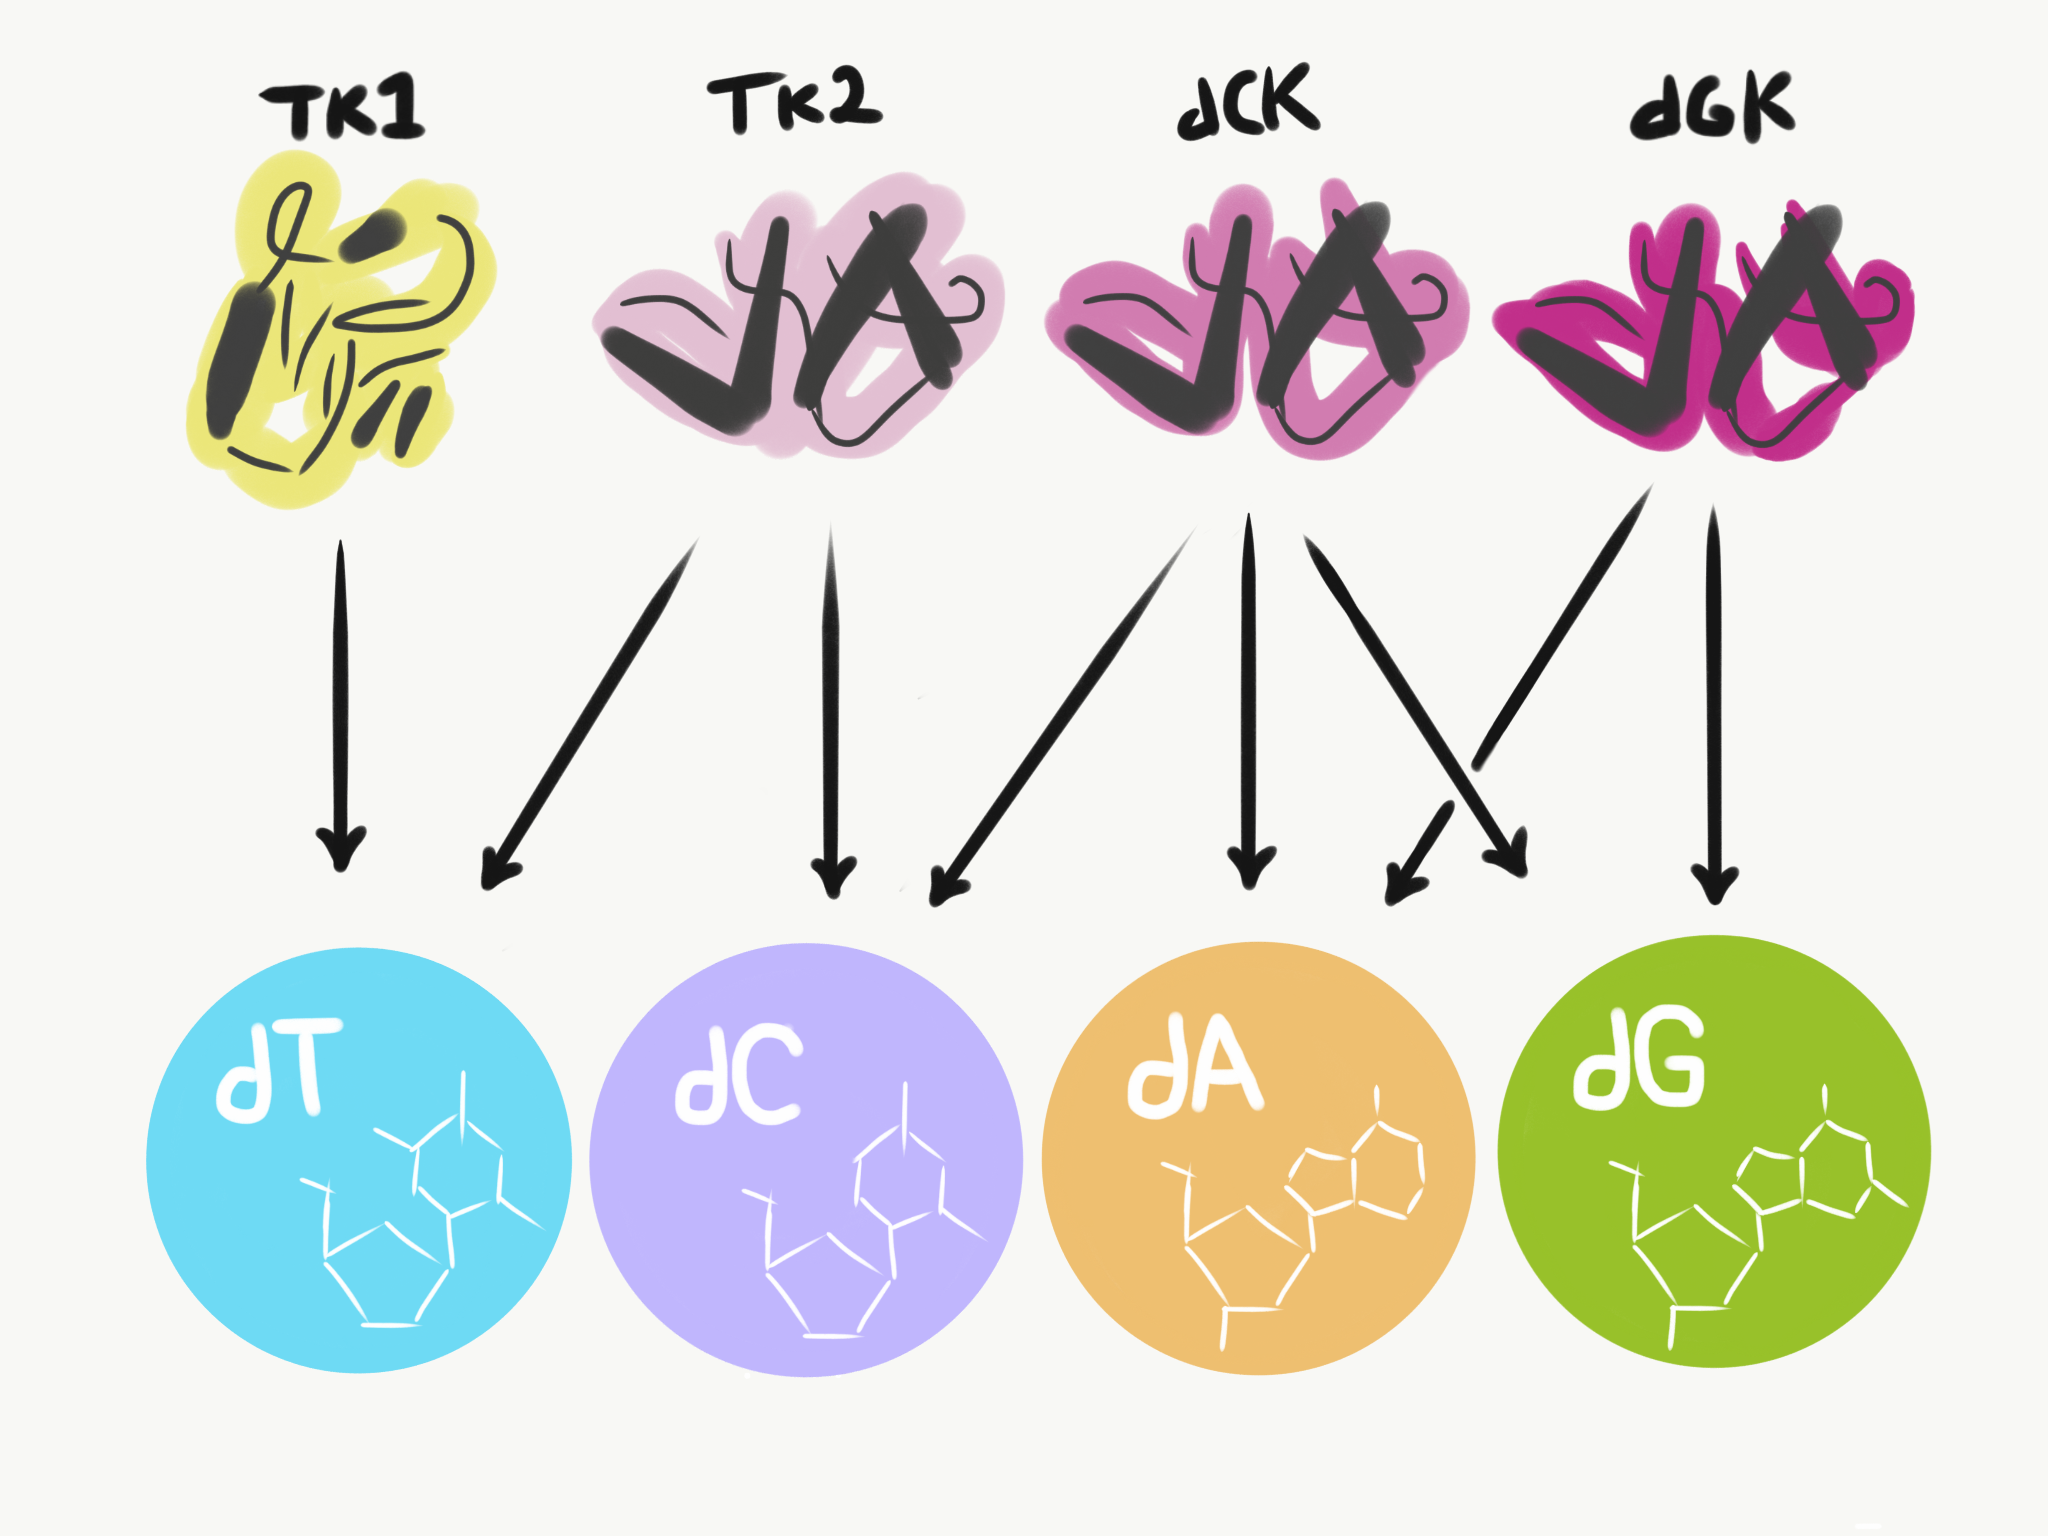
\includegraphics[width=\textwidth]{img/intraindividual_degeneracy}
 \end{column}
 \begin{column}{0.4\textwidth}
\captionsetup{singlelinecheck=off,justification=raggedright}
  	\caption{Mammalian deoxyribonucleoside kinases exhibit degeneracy \cite{Sandrini2005DeoxyribonucleosideReaction.}.}
    \label{fig:intraindividual_degeneracy}
    
\end{column}
\end{columns}
\end{figure}
\end{frame}


\section{Evolvability in Action}

\begin{frame}{Promoting Evolvability: Indirect Encoding}
  \begin{figure}
  \centering
  \begin{subfigure}[b]{0.5\textwidth}
    \centering
    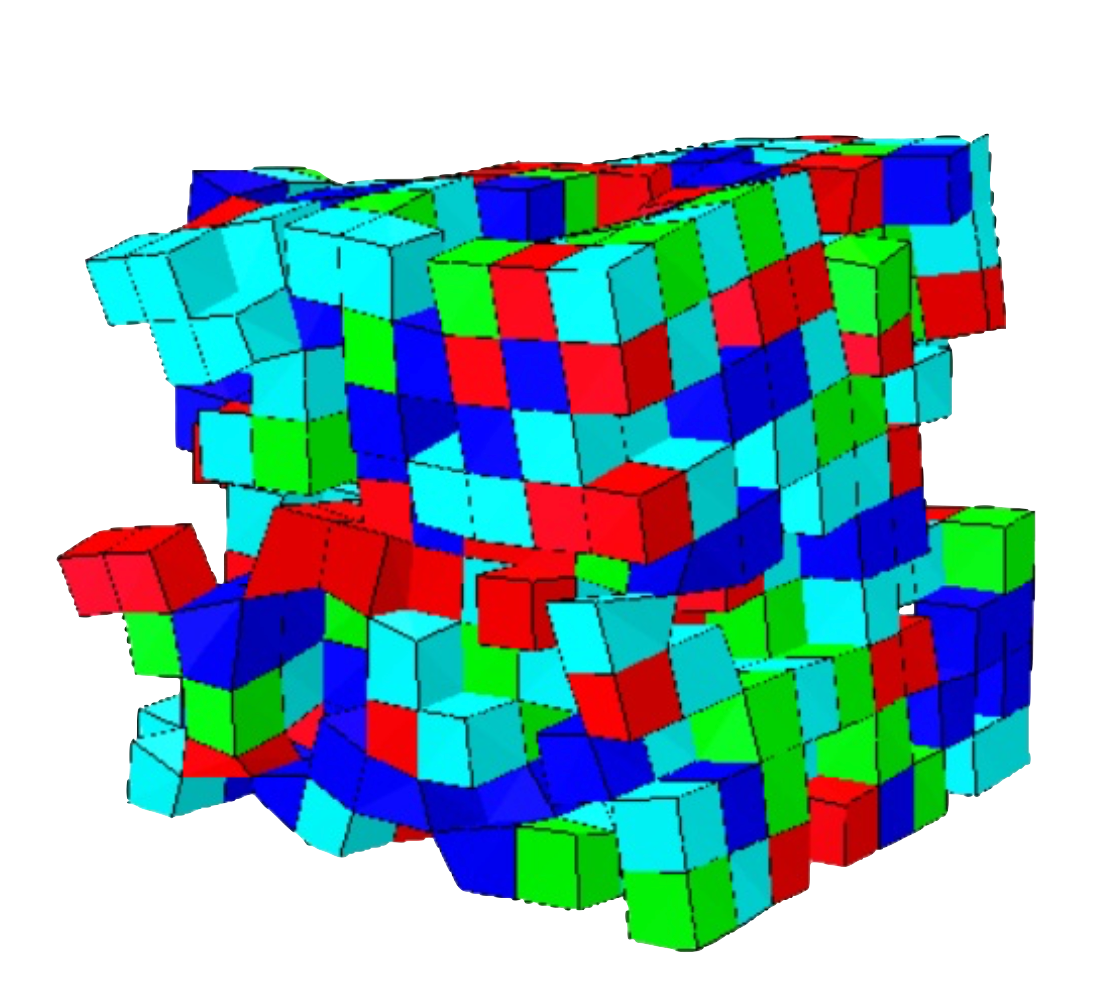
\includegraphics[width=\textwidth]{img/direct_encoding.png}
    \caption{direct encoding (low regularity)}
    \label{subfig:canalization}
  \end{subfigure}%
  \hfill
  \begin{subfigure}[b]{0.5\textwidth}
    \centering
    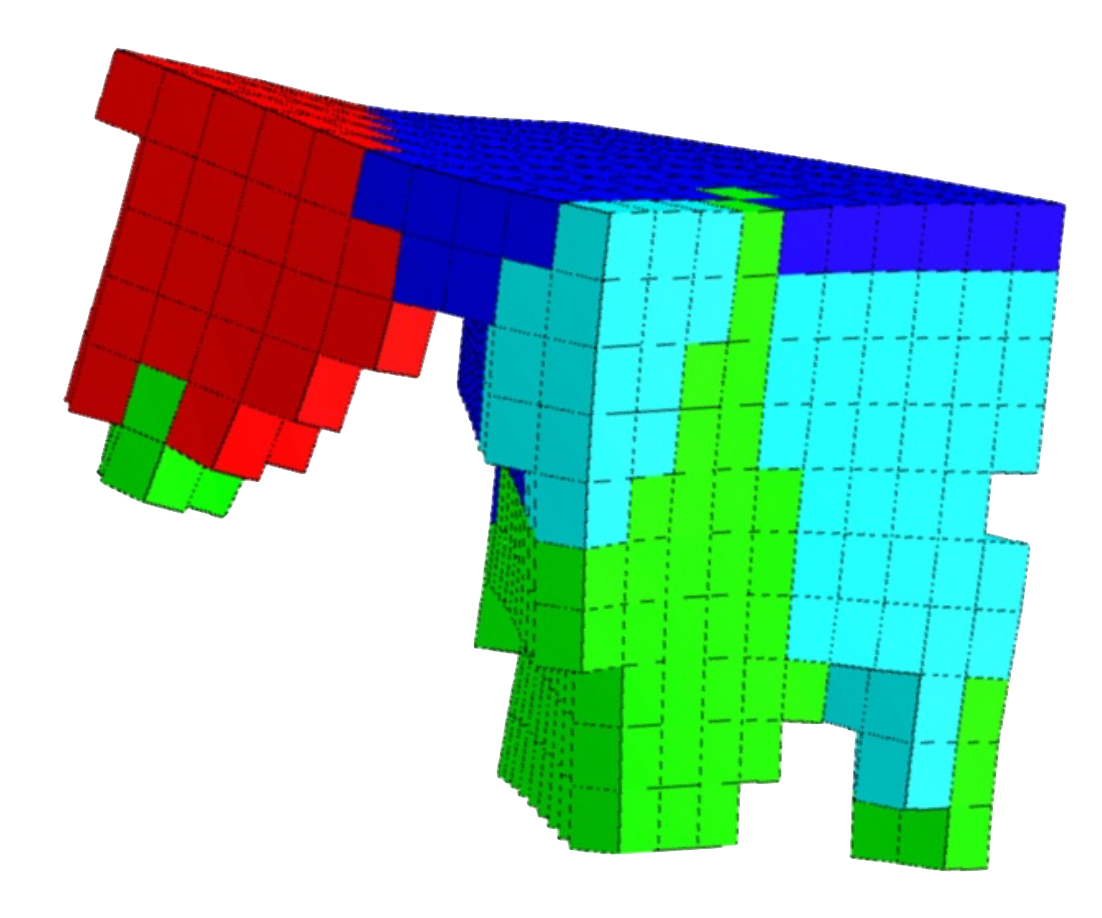
\includegraphics[width=\textwidth]{img/cppn-neat_encoded.png}
    \caption{indirect encoding (high regularity)}
  \end{subfigure}
  \captionsetup{singlelinecheck=off,justification=raggedright}
  \caption{Representative examples of soft robots evolved with direct and indirect representations \cite[Figures 6, 7]{Cheney2013UnshacklingEncoding}}
  \label{fig:direct_irregular_vs_indirect_regular}
\end{figure}
\end{frame}


\section{Plasticity}

\begin{frame}{Environmental Influence on the Phenotype}
\begin{itemize}
	\item in biology, genotype not sole determinant of phenotype
    \item $P = G + E$
    \item plasticity: phenotypic response to the environment
    \item direct plasticity versus indirect plasticity
\end{itemize}
\end{frame}

\begin{frame}{Direct Plasticity: Biological Intuition}
  \begin{figure} \label{fig:elephant_developmental_perturbation}
  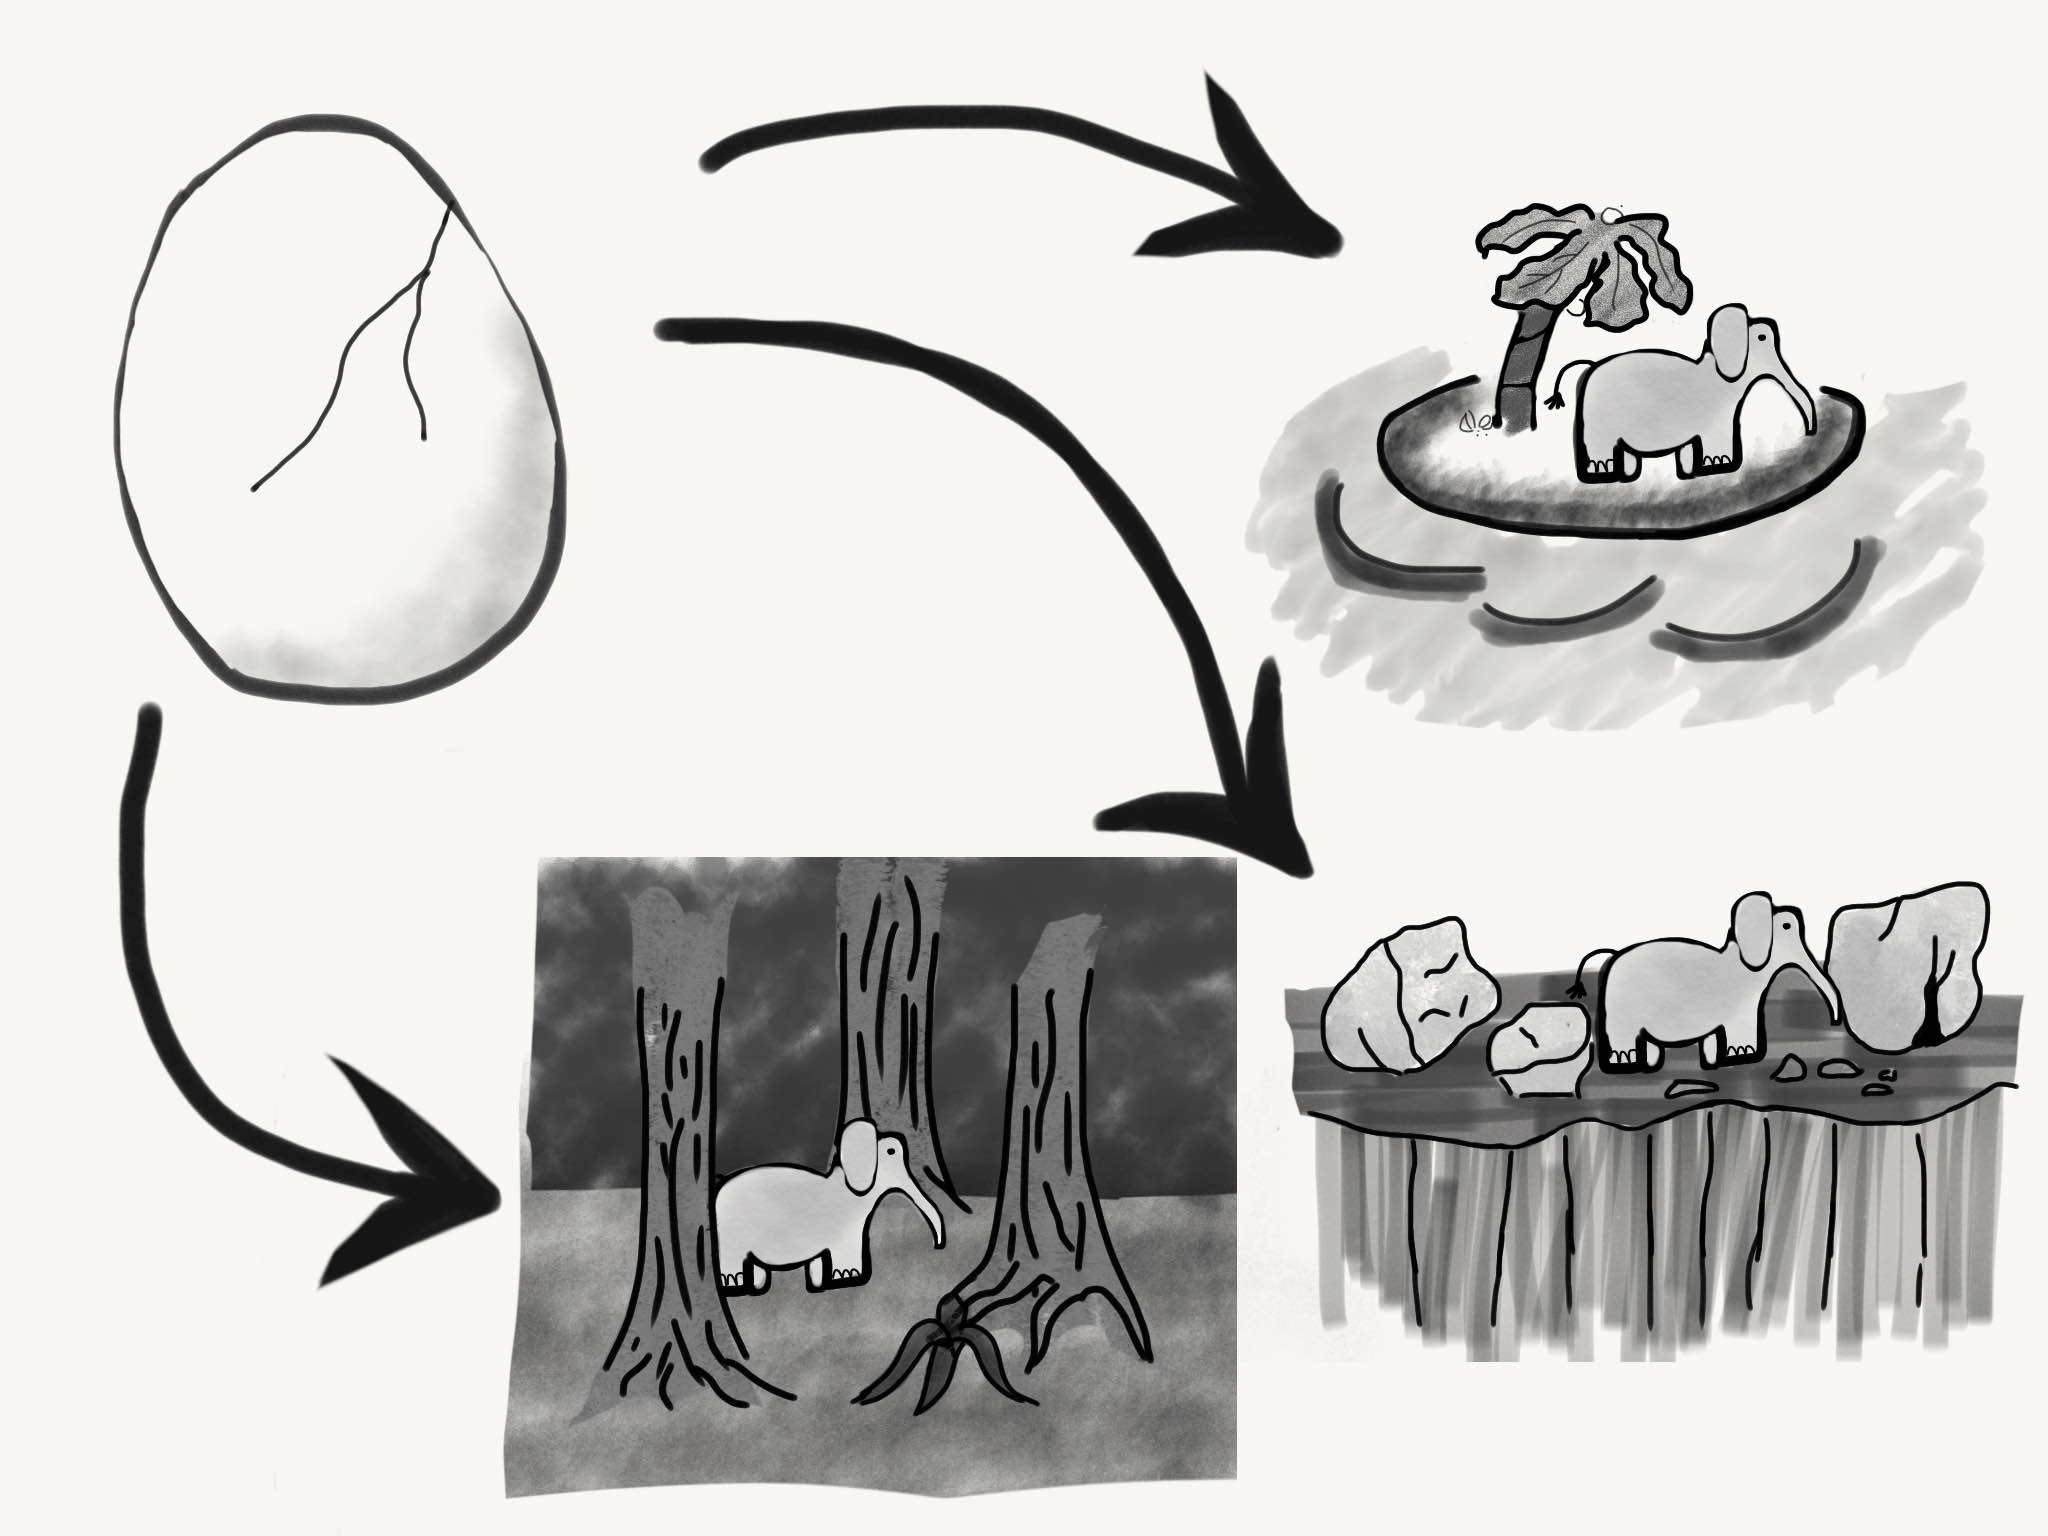
\includegraphics[width=0.8\textwidth]{img/elephant_developmental_perturbation.jpg}
  \captionsetup{singlelinecheck=off,justification=raggedright}

  \caption{A cartoon illustration of resistance to environmental perturbation.}
\end{figure}
\end{frame}

\begin{frame}{Indirect Plasticity: Biological Intuition}
  \begin{figure} \label{figs/plant_developmental_perturbation}
  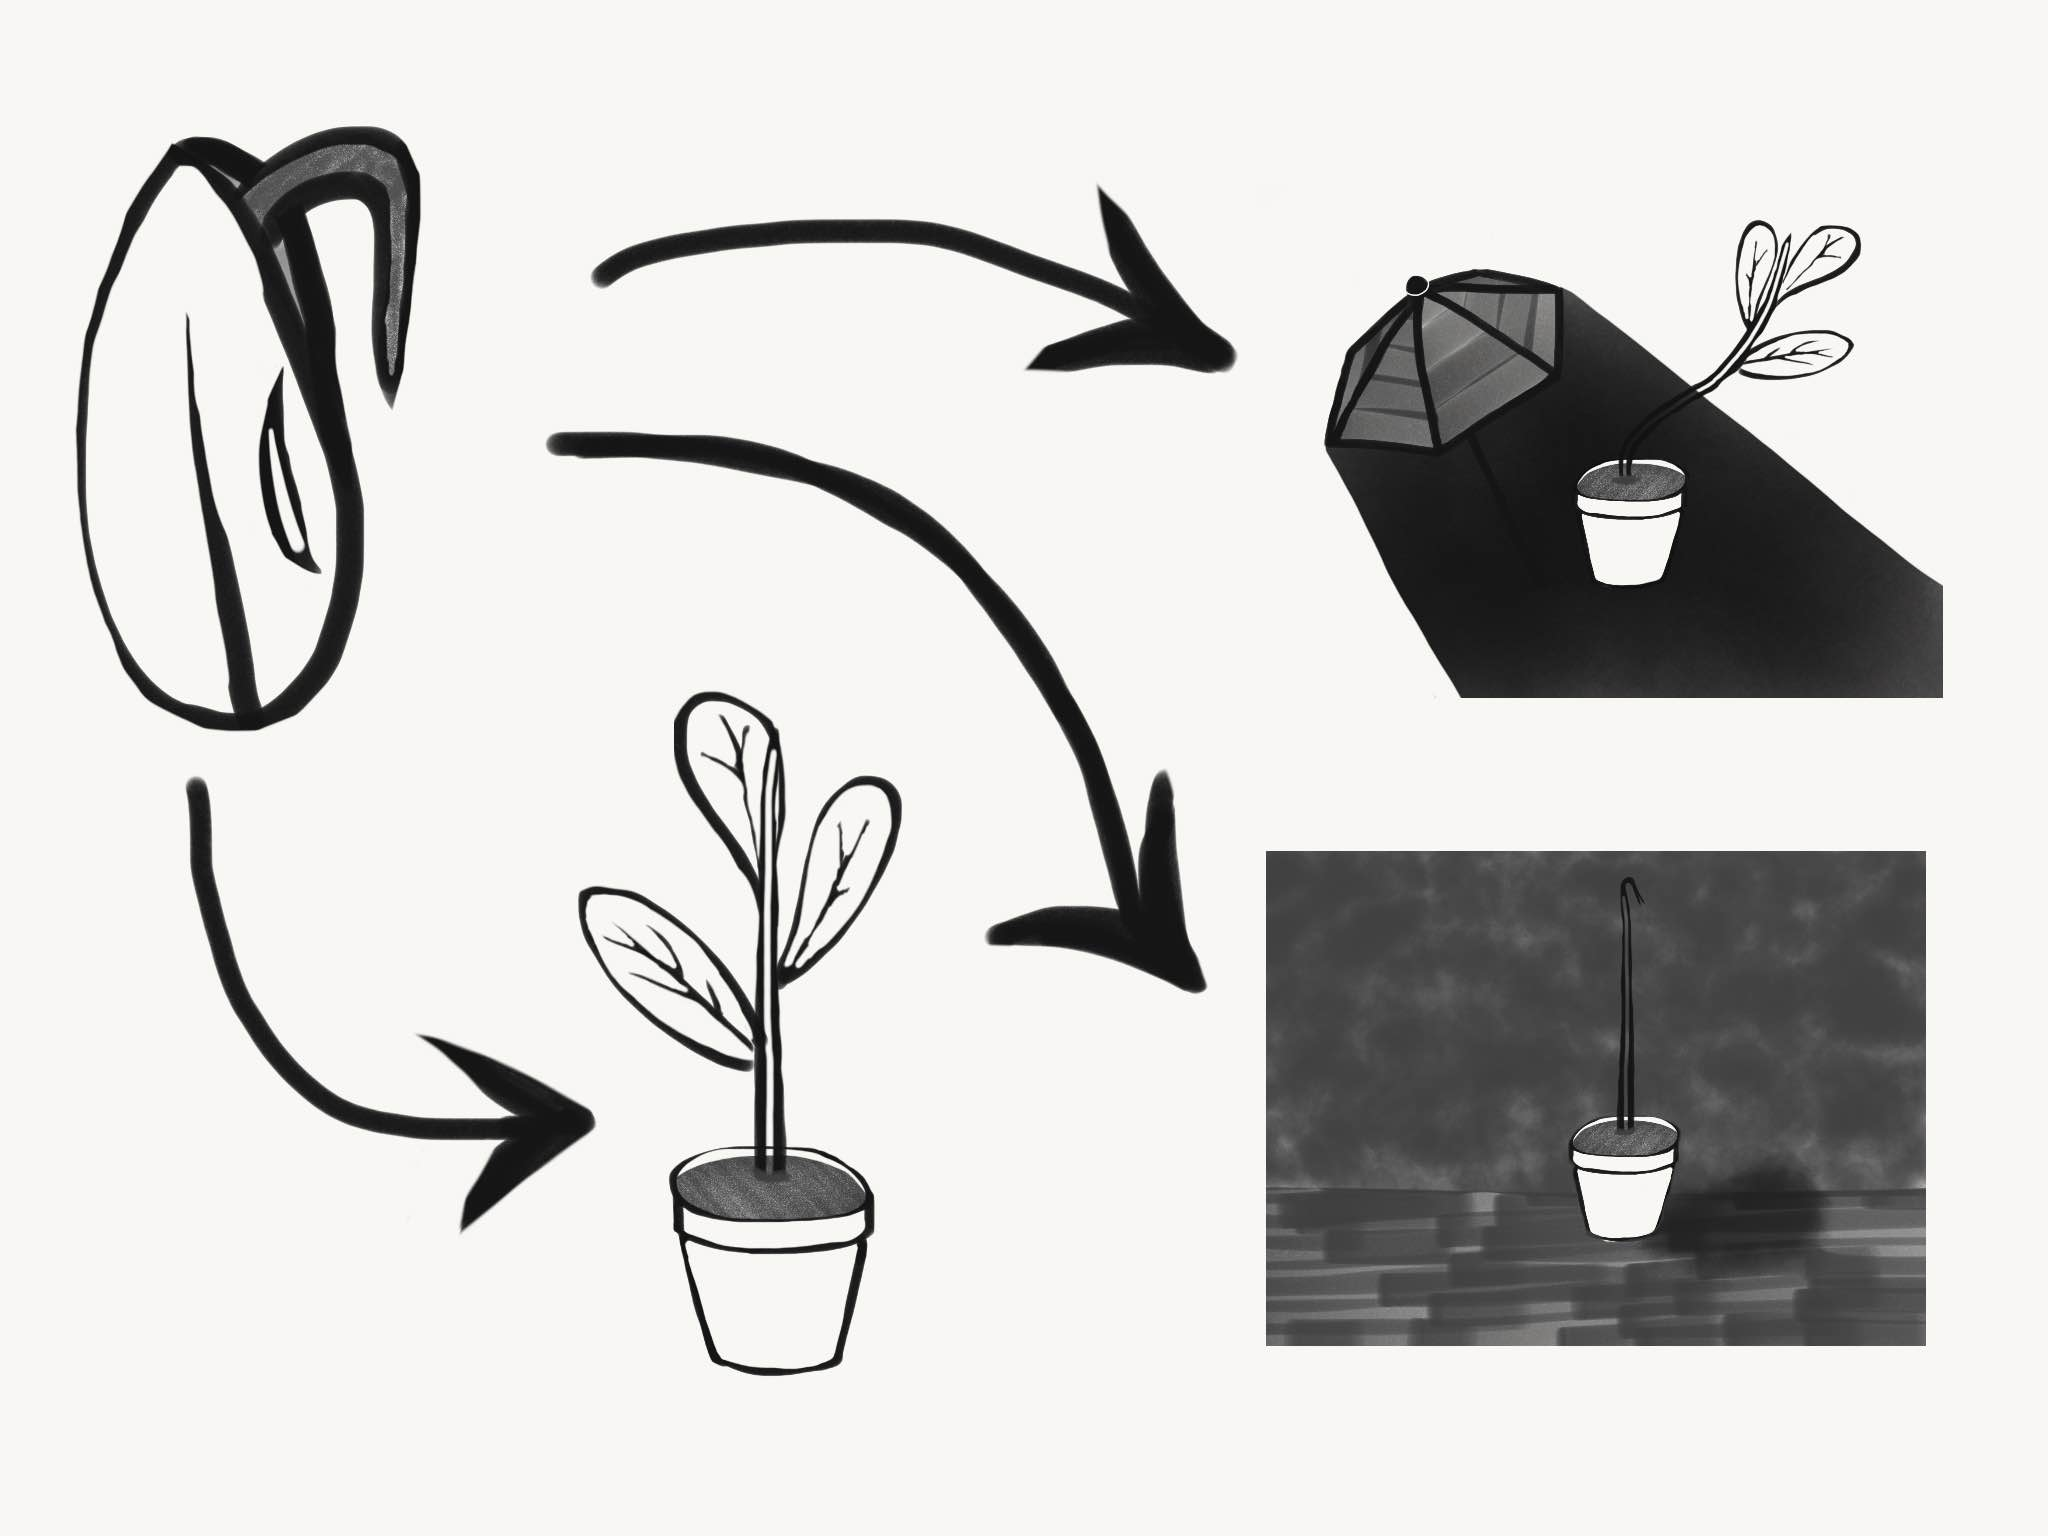
\includegraphics[width=0.8\textwidth]{img/plant_developmental_perturbation.jpg}
  \captionsetup{singlelinecheck=off,justification=raggedright}
  \caption{A cartoon illustration of alternate phenotypes expressed based on environmental signals.}
\end{figure}

\end{frame}


\section{Genetic Regulatory Network Model}

\begin{frame}{Model Framework}
\begin{columns}
\begin{column}{0.5\textwidth}
\begin{figure}
    \centering
    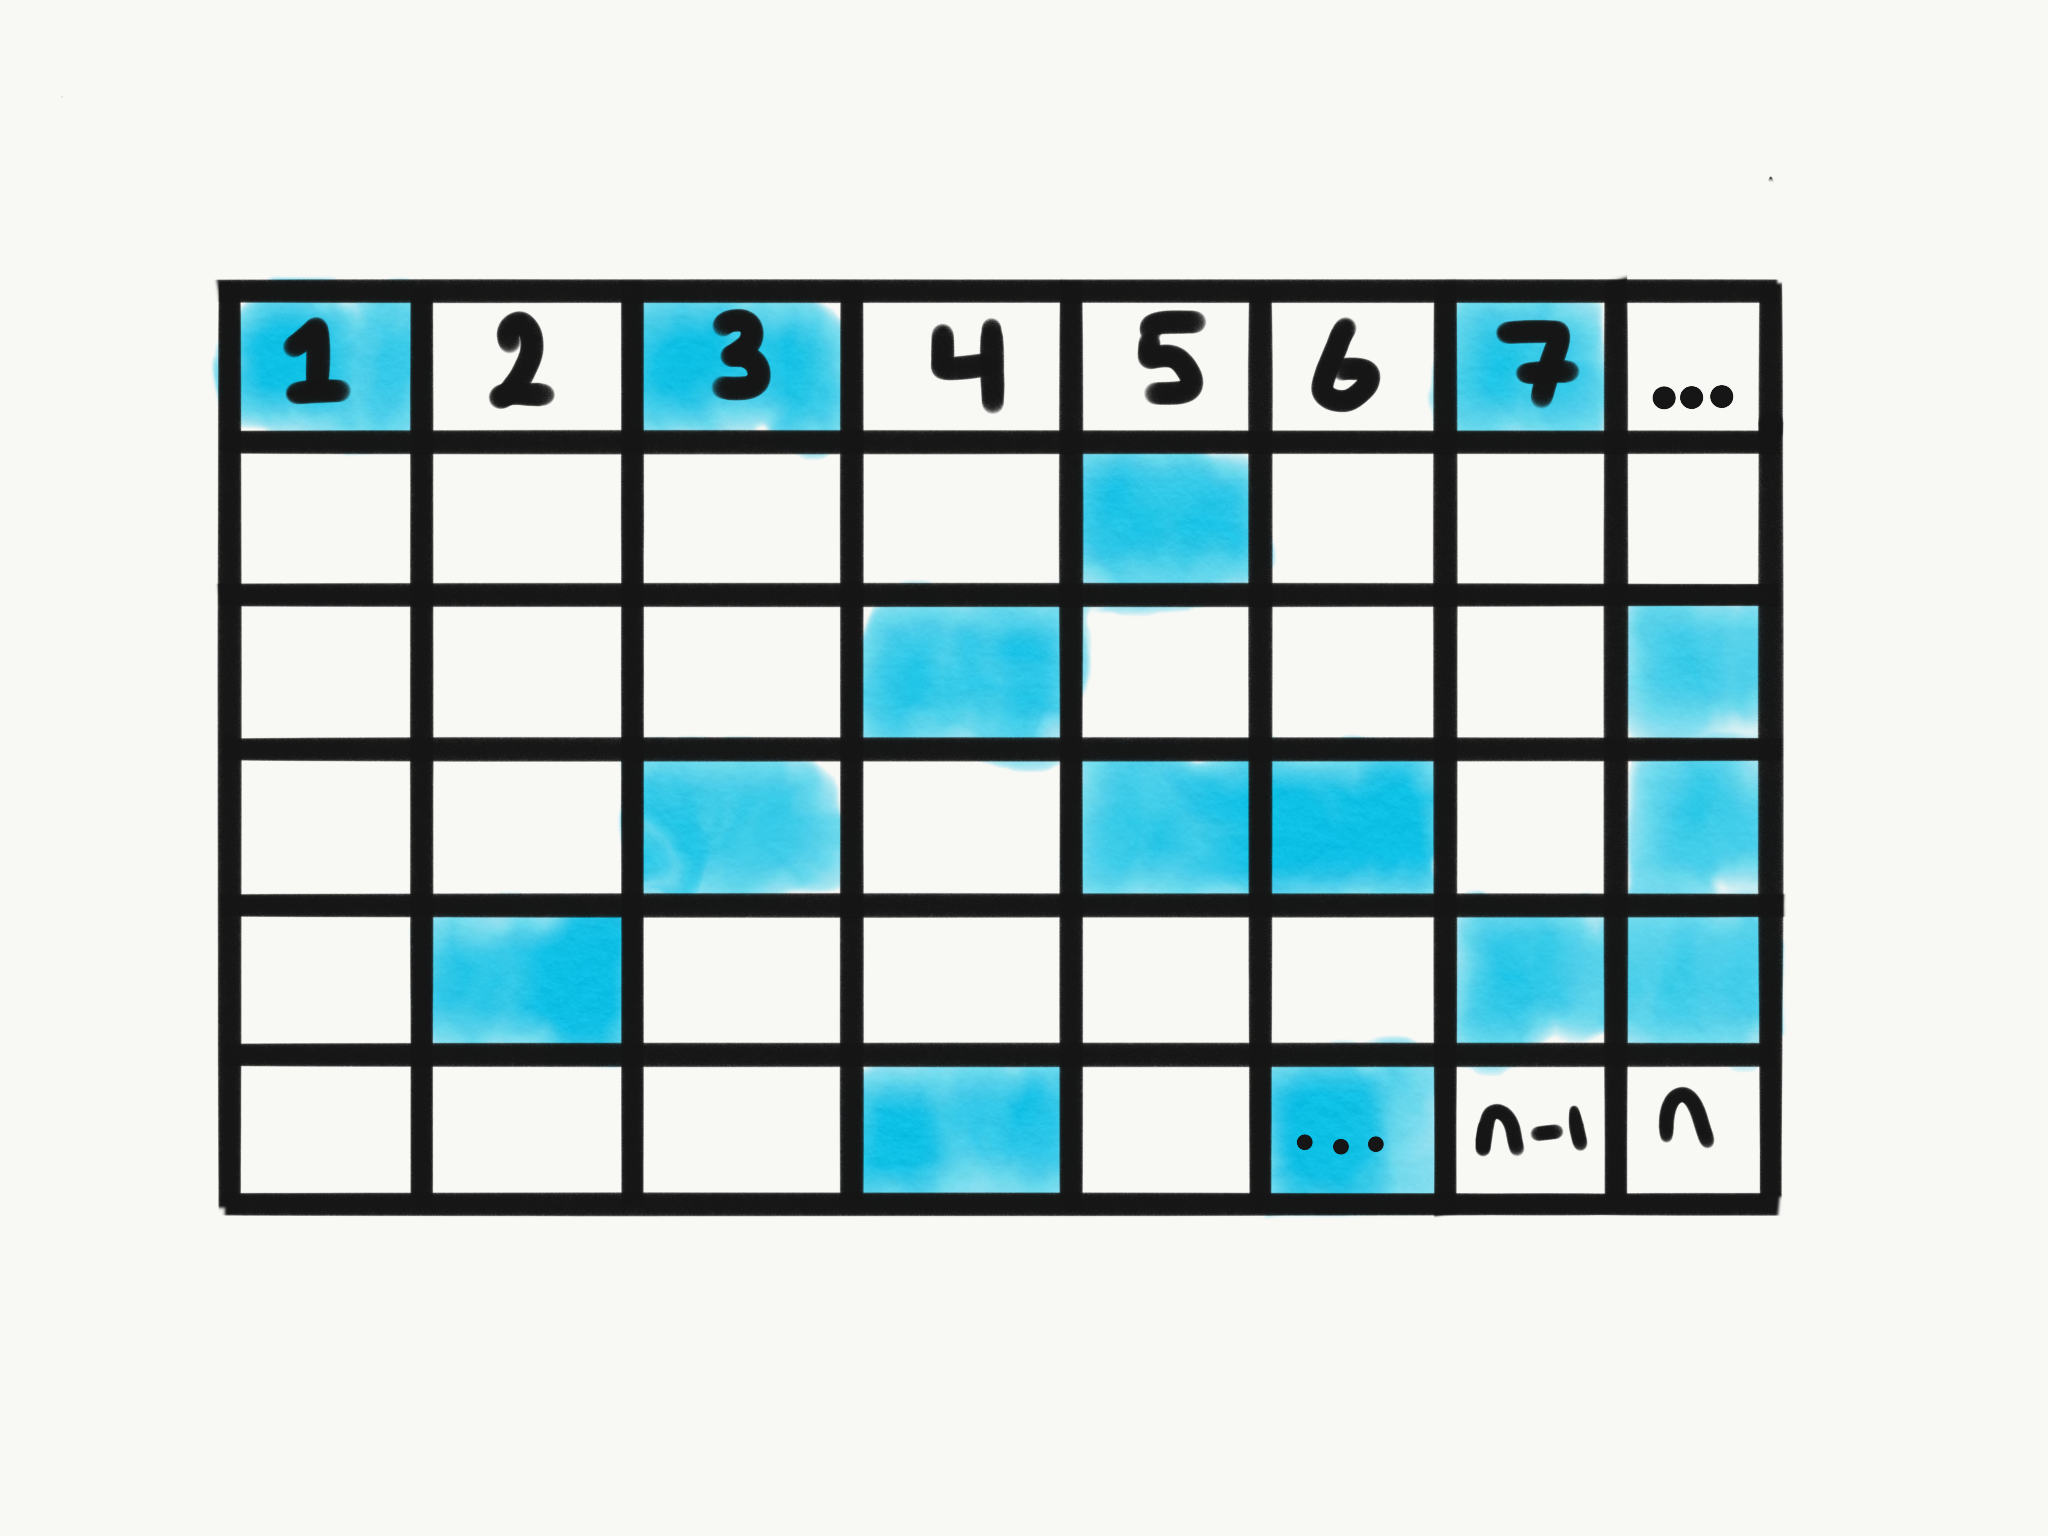
\includegraphics[width=\textwidth]{img/initial_state}
 	\captionsetup{singlelinecheck=off,justification=raggedright}
  	\caption{Chemical concentrations are represented as a list of boolean values.}
    \label{fig:initial_state}
\end{figure}
\end{column}

\begin{column}{0.5\textwidth}
\begin{figure}
    \centering
    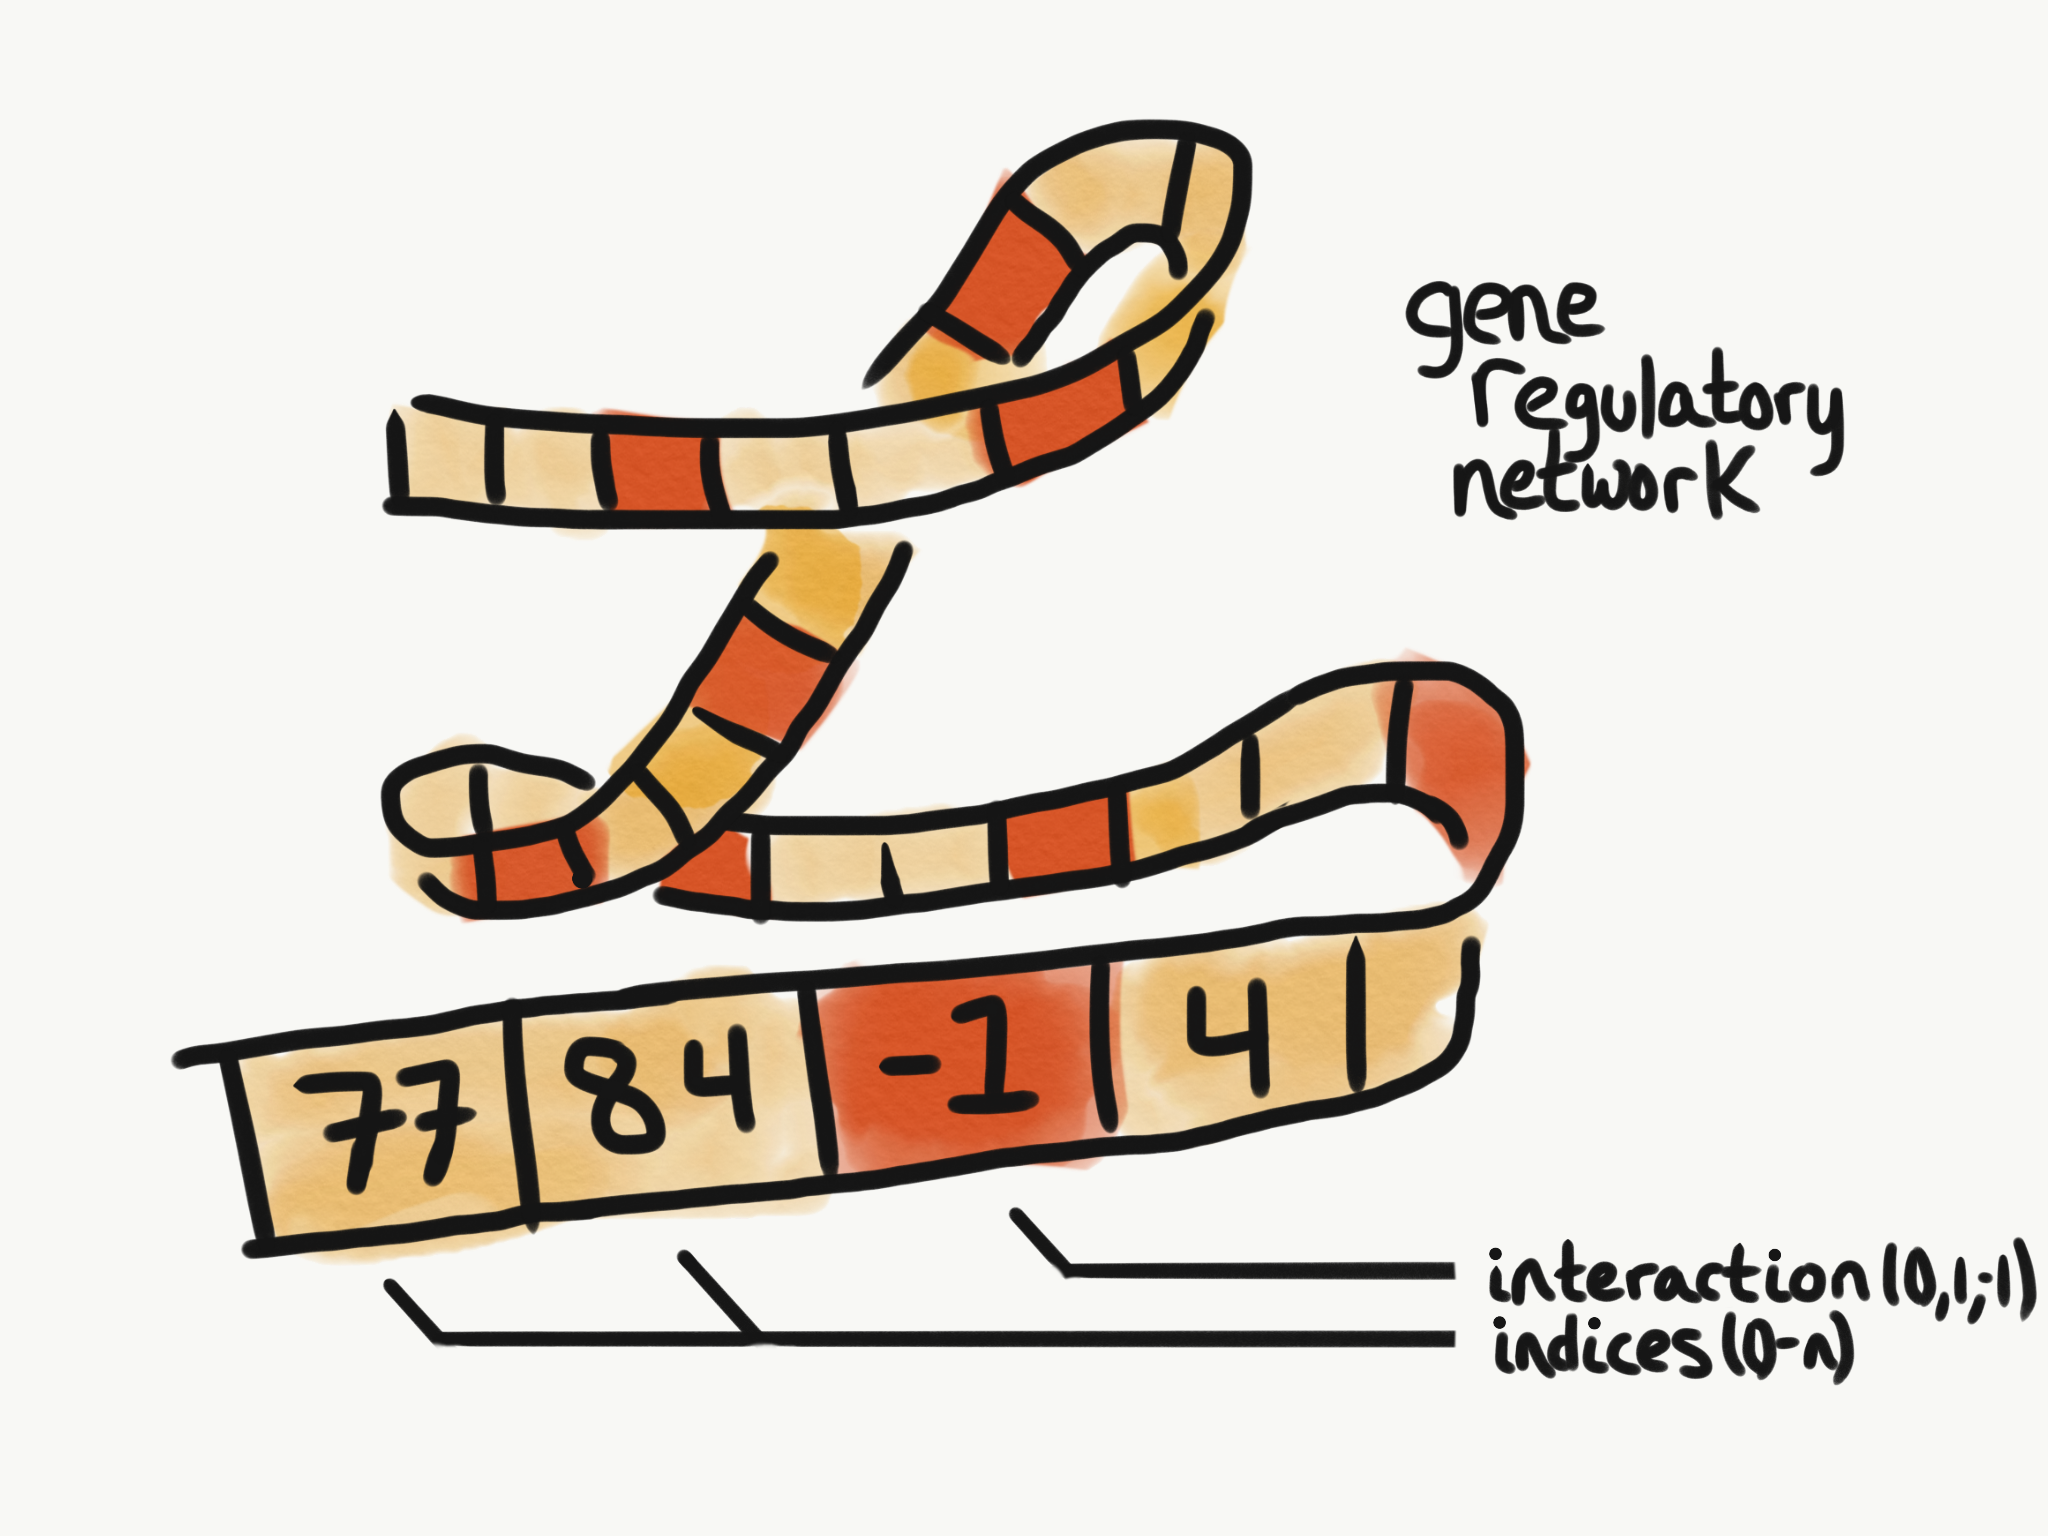
\includegraphics[width=\textwidth]{img/expanded_grn}
 	\captionsetup{singlelinecheck=off,justification=raggedright}
  	\caption{The GRN genotype is a set of if-then rules that acts on a set of chemical concentrations. The model employed was inspired by \cite{Wilder2015ReconcilingEvolvability}.}
    \label{fig:expanded_grn}
\end{figure}
\end{column}

\end{columns}
\end{frame}

\begin{frame}{Model Framework}
\begin{figure}
  \centering
  \begin{subfigure}[b]{\textwidth}
    \centering
    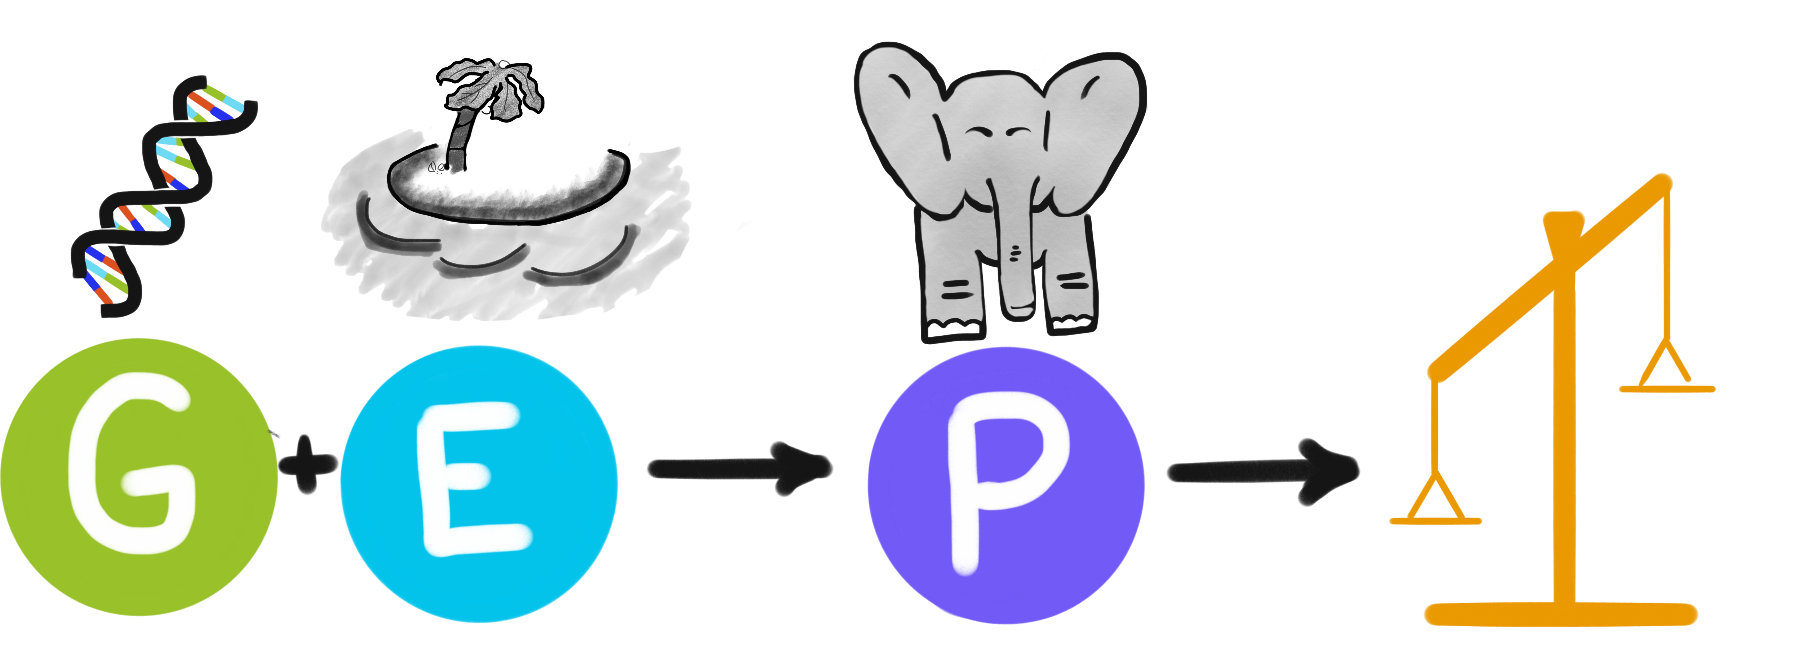
\includegraphics[width=0.6\textwidth]{img/bioscheme}
    \caption{biological inspiration}
    \label{subfig:bioscheme}
  \end{subfigure}
  \hfill
  \begin{subfigure}[b]{0.6\textwidth}
    \centering
    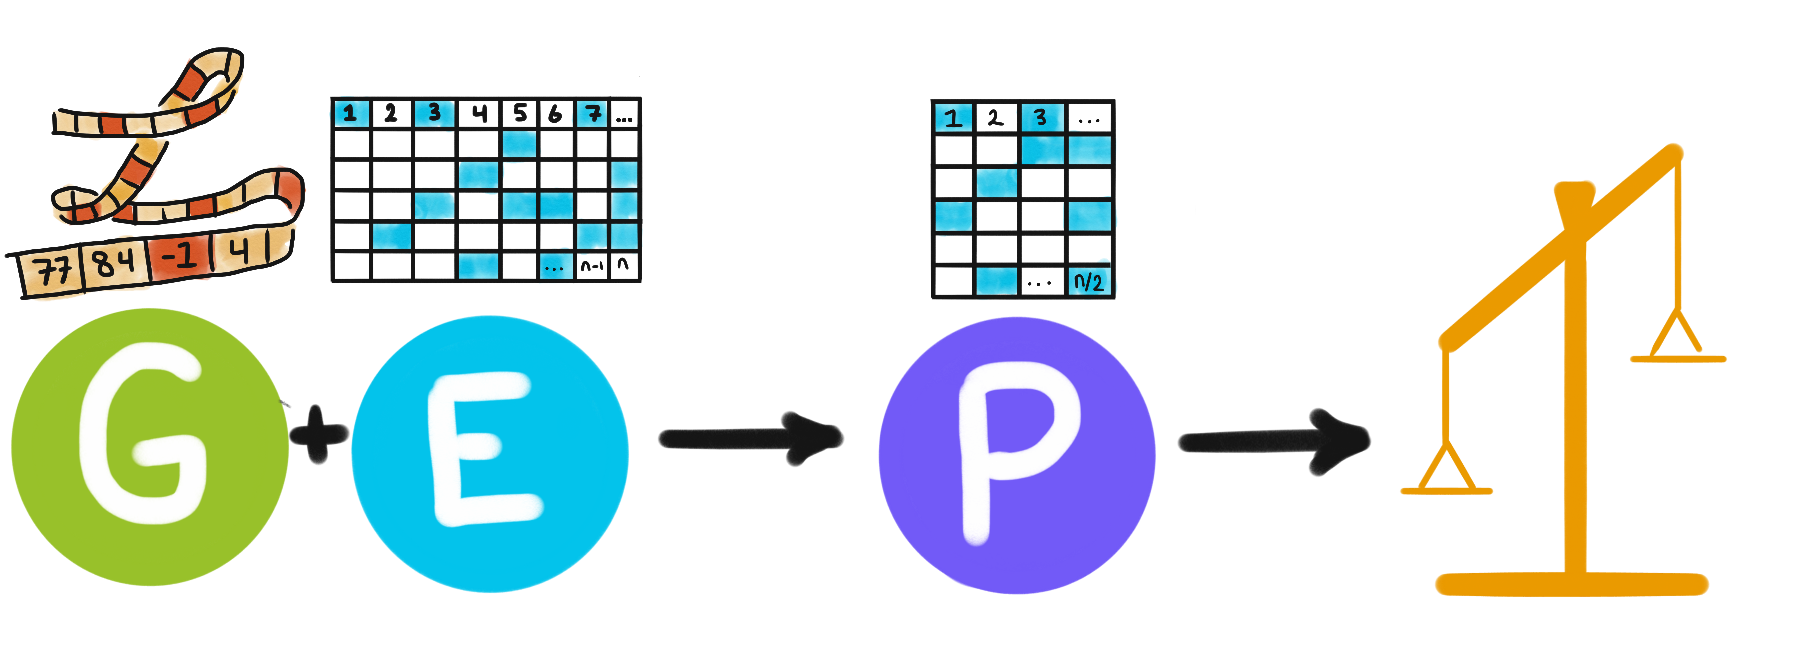
\includegraphics[width=\textwidth]{img/modelscheme}
    \caption{genetic regulatory network model}
     \label{subfig:modelscheme}
  \end{subfigure}
  \captionsetup{singlelinecheck=off,justification=raggedright}
  \caption{A comparison of the genetic regulatory network model and its biological inspiration.}
  \label{fig:model_bio_comparison}
\end{figure}
\end{frame}






\section{Experiment: Direct Plasticity}


\begin{frame}{Direct Plasticity: Initial State Perturbation}
\begin{figure}
  \centering
  \begin{subfigure}[b]{\textwidth}
    \centering
    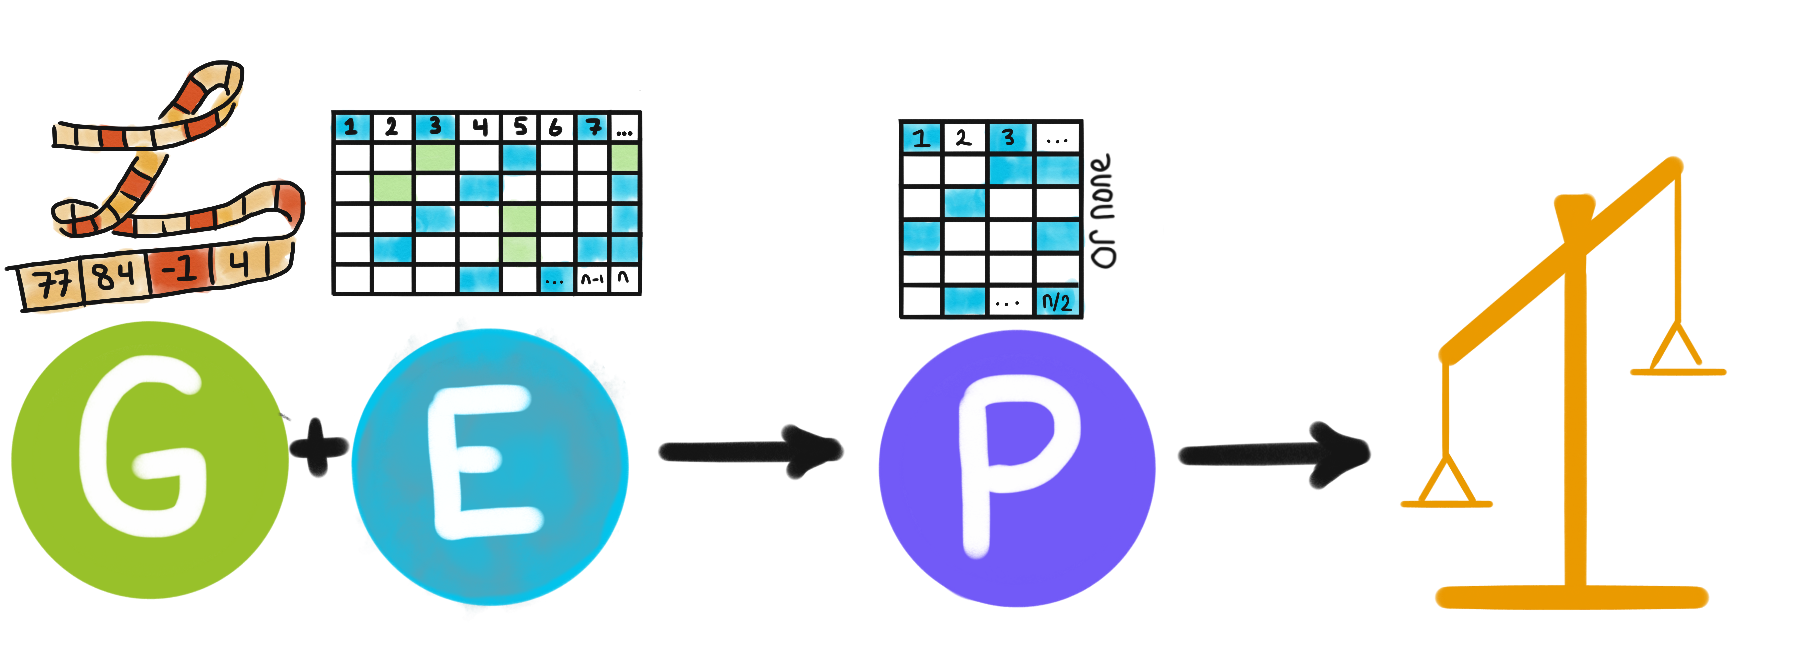
\includegraphics[width=0.6\textwidth]{img/directscheme}
    \caption{experimental scheme}
    \label{subfig:directscheme}
  \end{subfigure}
  \hfill
  \begin{subfigure}[b]{0.6\textwidth}
    \centering
    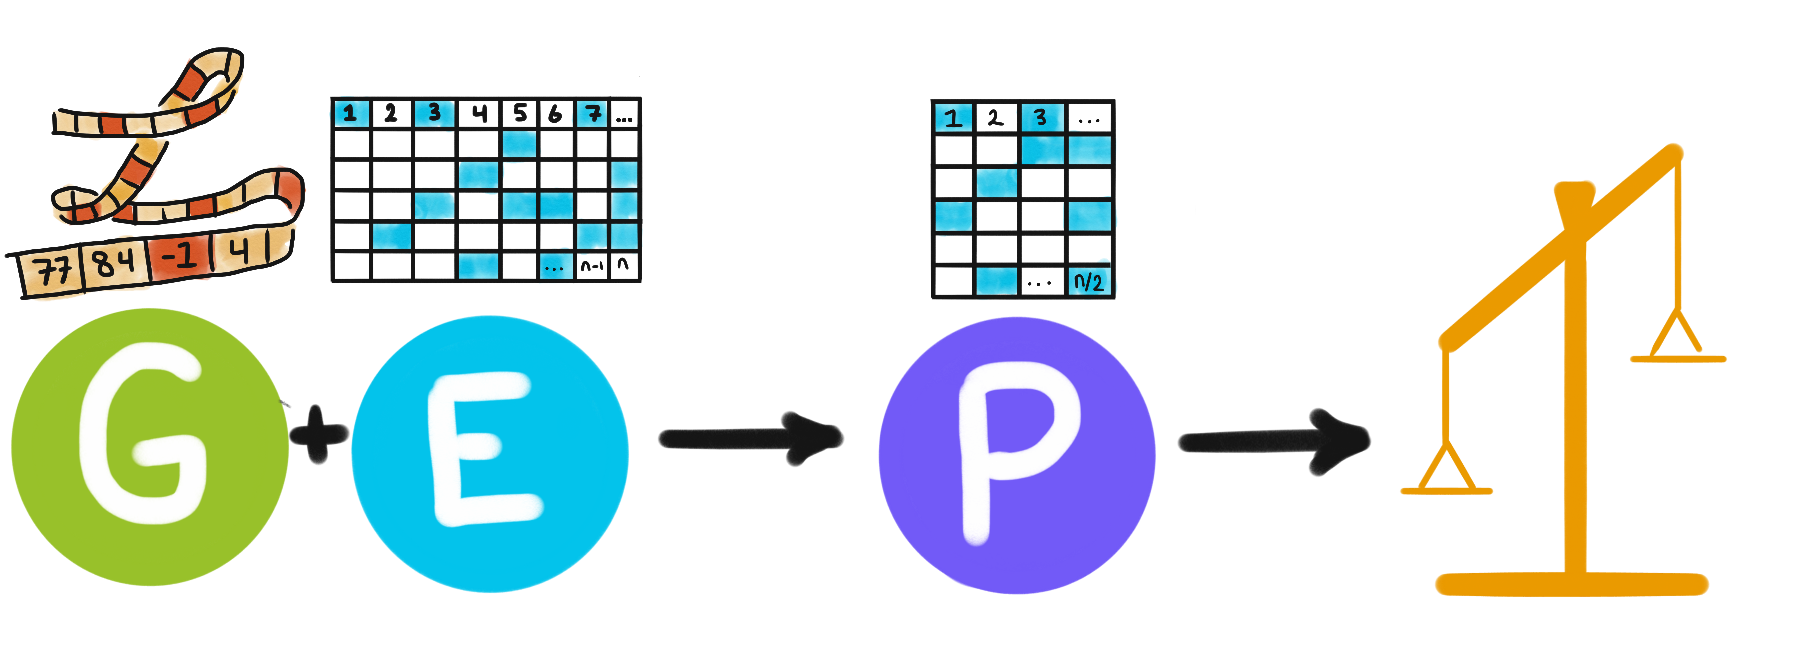
\includegraphics[width=\textwidth]{img/modelscheme}
    \caption{control scheme}
     \label{subfig:controlscheme}
  \end{subfigure}
  \captionsetup{singlelinecheck=off,justification=raggedright}
  \caption{A comparison of the control and experimental schemes employed to investigate the relationship between direct plasticity and evolvability.}
  \label{fig:direct_plasticity_scheme}
\end{figure}
\end{frame}

\begin{frame}{Evolvability Signature $P=0$}
\begin{figure}
    \centering
    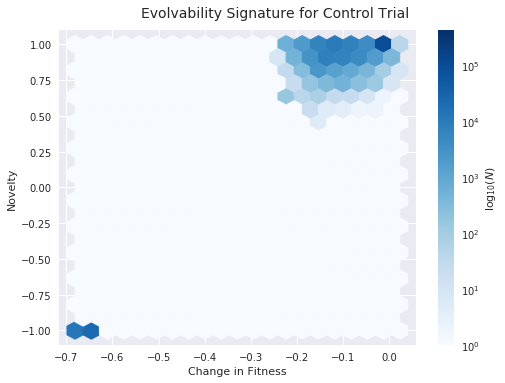
\includegraphics[width=0.8\textwidth]{img/es_p0}
 	\captionsetup{singlelinecheck=off,justification=raggedright}
  	\caption{Evolvability signature of champion evolved with no initial plasticity. Figure after \cite{Tarapore2015EvolvabilityBenchmarks}.}
    \label{fig:es_p0}
\end{figure}
\end{frame}

\begin{frame}{Evolvability Signature $P=0.1$}
\begin{figure}
    \centering
    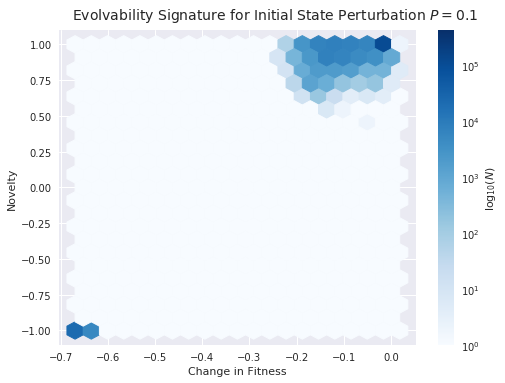
\includegraphics[width=0.8\textwidth]{img/es_p0_1}
 	\captionsetup{singlelinecheck=off,justification=raggedright}
  	\caption{Evolvability signature of champion evolved with medium initial plasticity, $P=0.1$. Figure after \cite{Tarapore2015EvolvabilityBenchmarks}.}
    \label{fig:es_p0_1}
\end{figure}
\end{frame}

\begin{frame}{Evolvability Signature $P=0.2$}
\begin{figure}
    \centering
    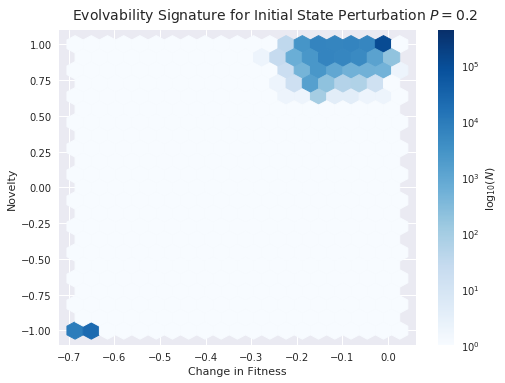
\includegraphics[width=0.8\textwidth]{img/es_p0_2}
 	\captionsetup{singlelinecheck=off,justification=raggedright}
  	\caption{Evolvability signature of champion evolved with greater initial plasticity, $P=0.2$. Figure after \cite{Tarapore2015EvolvabilityBenchmarks}.}
    \label{fig:es_p0_2}
\end{figure}
\end{frame}

\begin{frame}{Mutational Outcome Frequencies}
\begin{figure}
    \centering
    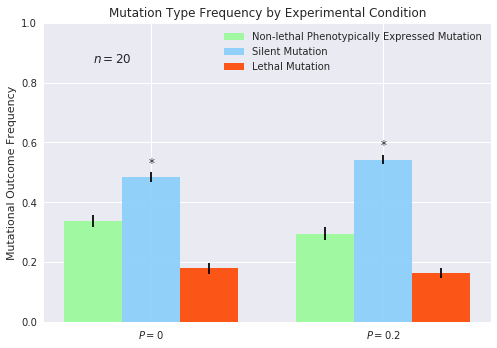
\includegraphics[width=0.8\textwidth]{img/mutation_type_direct}
 	\captionsetup{singlelinecheck=off,justification=raggedright}
  	\caption{Comparison of mutational outcome frequencies for champions evolved with and without initial state perturbation.}
    \label{fig:mutation_type_indirect}
\end{figure}
\end{frame}

\begin{frame}{Direct Plasticity Results: Summary}
\begin{itemize}
  \item direct plasticity increases robustness to mutation
  \item as in \cite{Reisinger2005TowardsEvolvability}, repeated evaluations ($n=10$) were required to observe impact of direct plasticity
  \item direct plasticity does not seem to promote canalization 
\end{itemize}
\end{frame}

\section{Experiment: Indirect Plasticity}

\begin{frame}{Indirect Plasticity: Conditional Initial State}
\begin{figure}
  \centering
  \begin{subfigure}[b]{\textwidth}
    \centering
    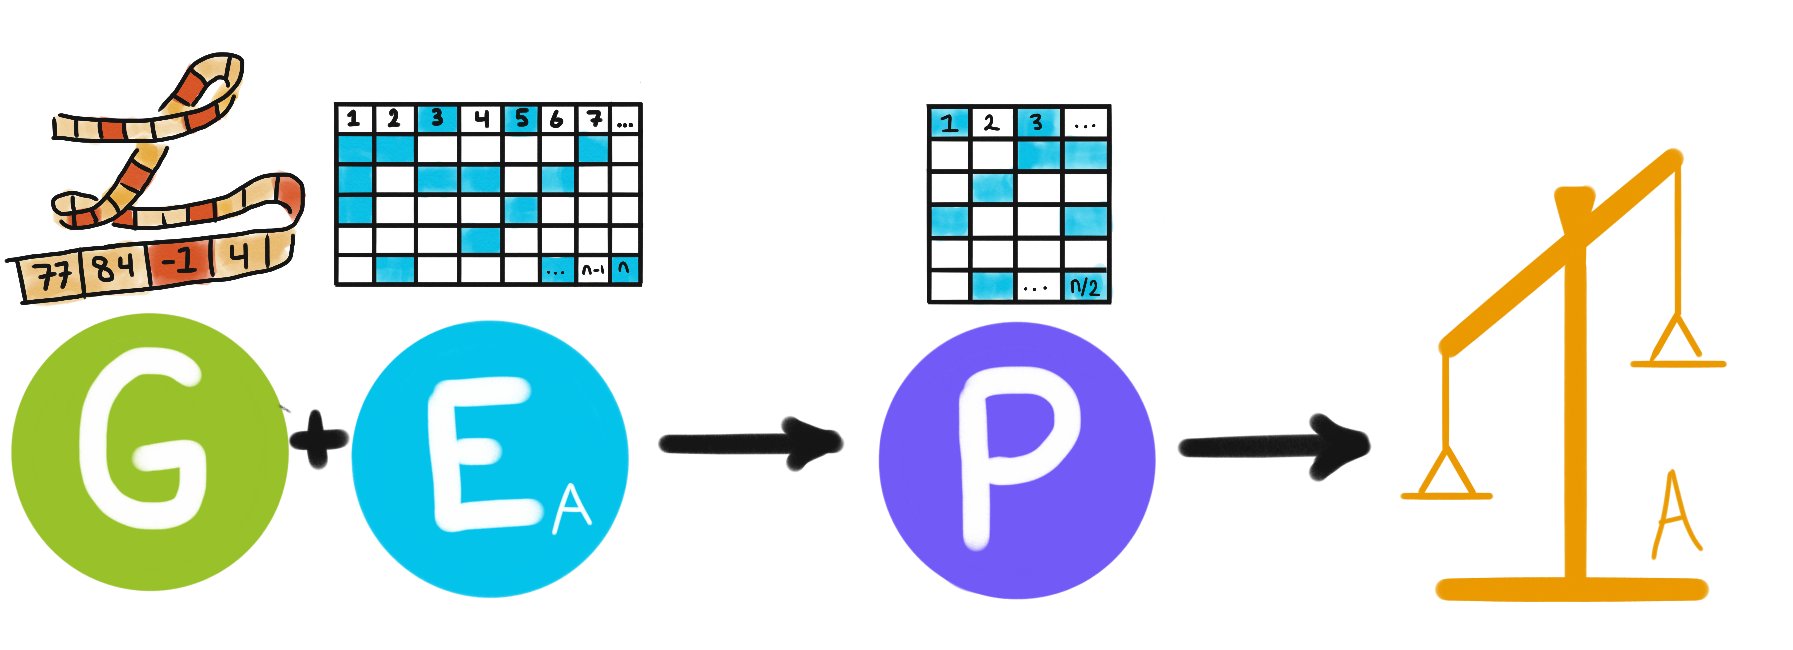
\includegraphics[width=0.4\textwidth]{img/indirectschemeA} \\
    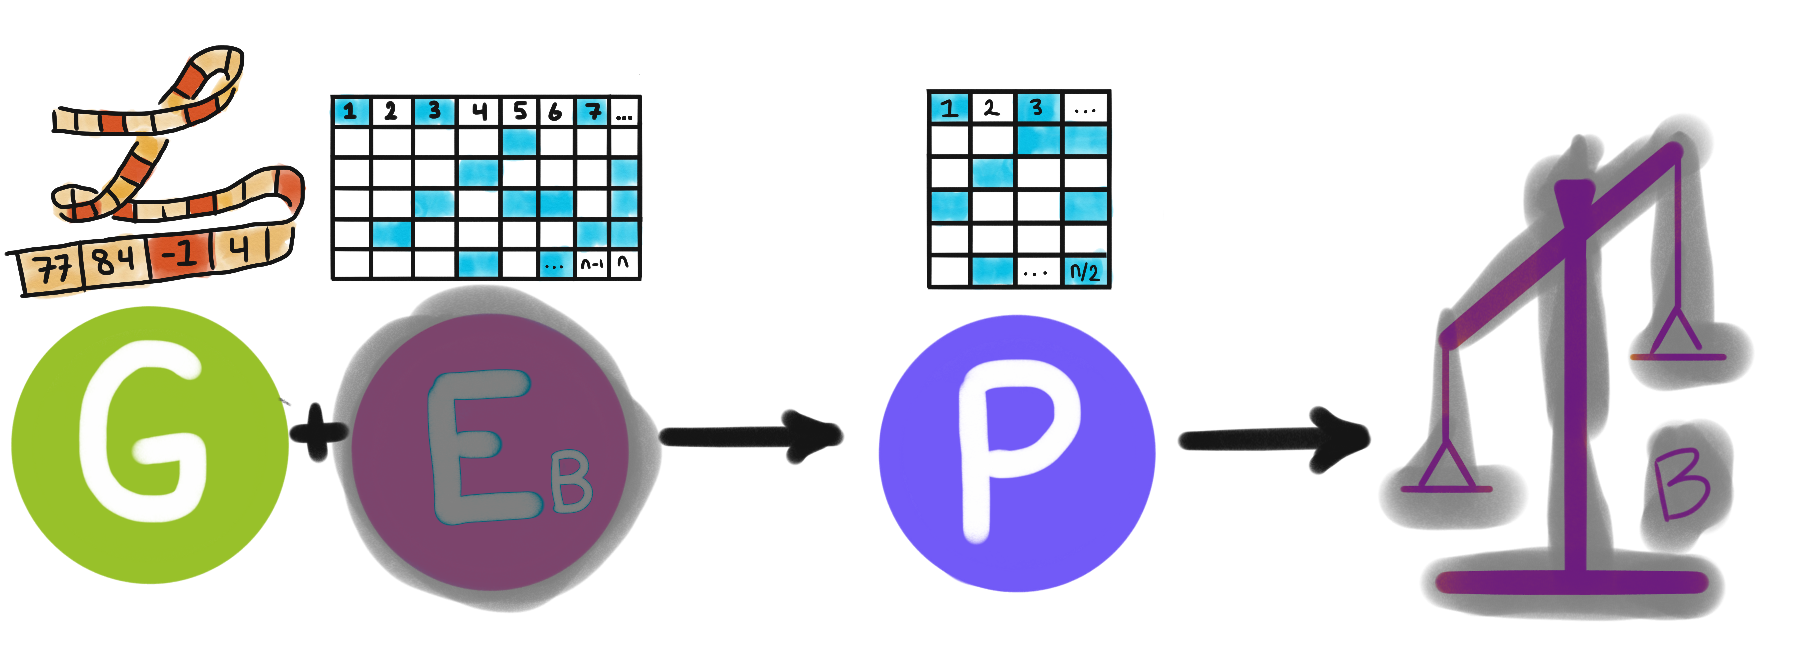
\includegraphics[width=0.4\textwidth]{img/indirectschemeB}
    \caption{experimental scheme}
    \label{subfig:directscheme}
  \end{subfigure}
  \hfill
  \begin{subfigure}[b]{\textwidth}
    \centering
    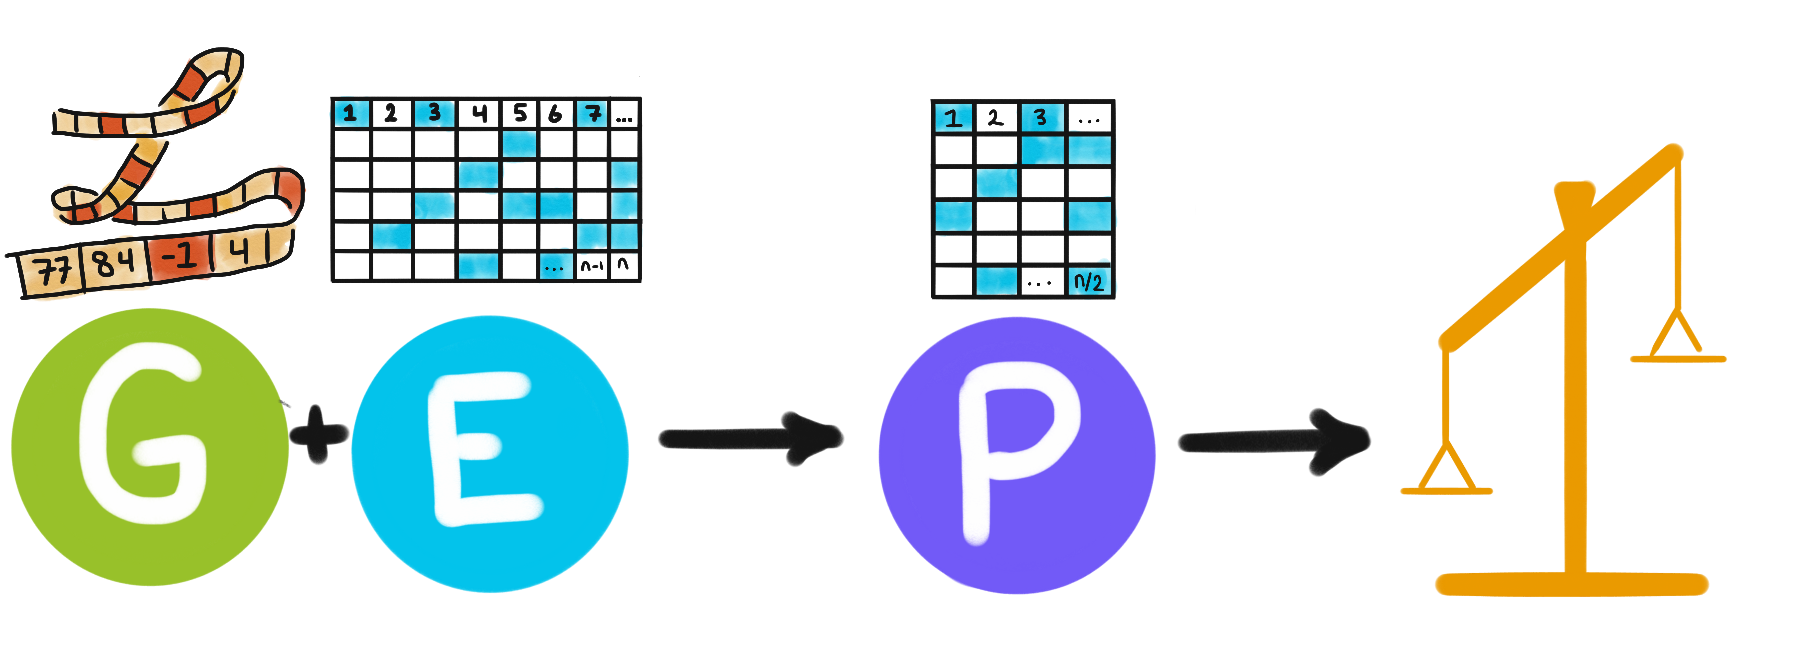
\includegraphics[width=0.4\textwidth]{img/modelscheme}
    \caption{control scheme}
     \label{subfig:controlscheme}
  \end{subfigure}
  \captionsetup{singlelinecheck=off,justification=raggedright}
  \caption{A comparison of the control and experimental schemes employed to investigate the relationship between indirect plasticity and evolvability.}
  \label{fig:direct_plasticity_scheme}
\end{figure}
\end{frame}

\begin{frame}{Evidence for Indirect Plasticity}
\begin{figure}
    \centering
    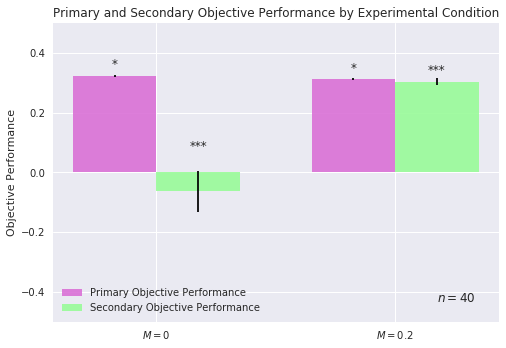
\includegraphics[width=0.8\textwidth]{img/primary_secondary_performance}
 	\captionsetup{singlelinecheck=off,justification=raggedright}
  	\caption{Comparison of objective performances of champions evolved with only primary condition/objective pair versus with both primary and secondary condition/objective pairs.}
    \label{fig:ev_w0}
\end{figure}
\end{frame}

\begin{frame}{Evolvability Visualization $W=0$}
\begin{figure}
    \centering
    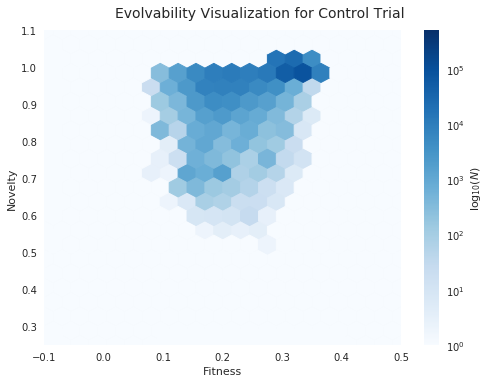
\includegraphics[width=0.8\textwidth]{img/ev_w0}
 	\captionsetup{singlelinecheck=off,justification=raggedright}
  	\caption{Evolvability visualization of champions evolved with only a primary condition/objective pair.}
    \label{fig:ev_w0}
\end{figure}
\end{frame}

\begin{frame}{Evolvability Visualization $W=0.2$}
\begin{figure}
    \centering
    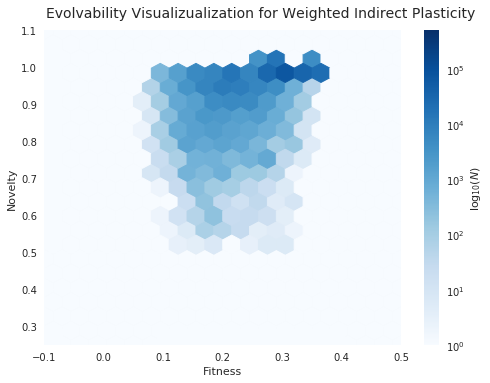
\includegraphics[width=0.8\textwidth]{img/ev_w0_2}
 	\captionsetup{singlelinecheck=off,justification=raggedright}
  	\caption{Evolvability visualization of champions evolved with primary and secondary condition/objective pairs.}
    \label{fig:es_w0_2}
\end{figure}
\end{frame}

\begin{frame}{Mutational Outcome Frequencies}
\begin{figure}
    \centering
    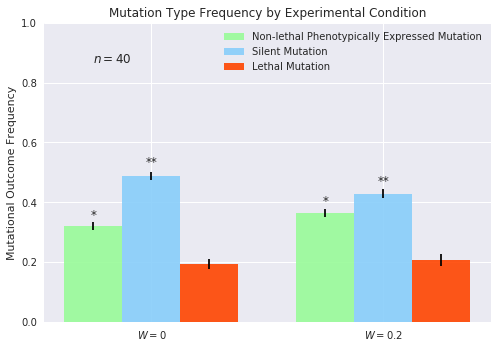
\includegraphics[width=0.8\textwidth]{img/mutation_type_indirect}
 	\captionsetup{singlelinecheck=off,justification=raggedright}
  	\caption{Comparison of mutational outcome frequencies for champions evolved with only primary condition/objective pair versus with both primary and secondary condition/objective pairs.}
    \label{fig:mutation_type_indirect}
\end{figure}
\end{frame}

\begin{frame}{Frequency of Useful Novelty}
 
 \begin{figure}
 \begin{subfigure}[b]{0.5\textwidth}
    \centering
    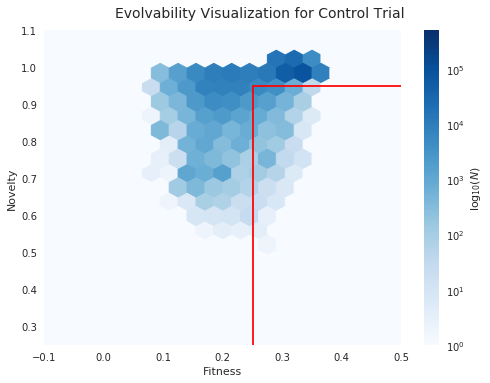
\includegraphics[width=\textwidth]{img/ev_w0_target}
    \caption{evolved with only primary condition/objective pair}
    \label{subfig:primary_only}
  \end{subfigure}%
    \begin{subfigure}[b]{0.5\textwidth}
    \centering
    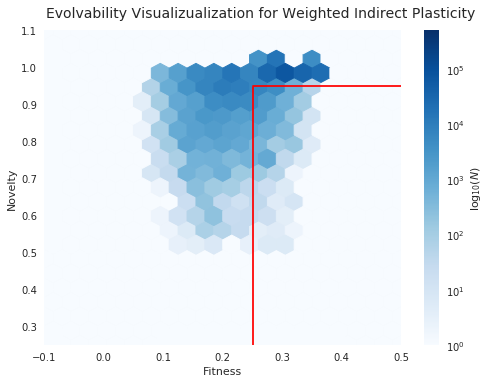
\includegraphics[width=\textwidth]{img/ev_w0_2_target}
    \caption{evolved with both primary and secondary condition/objective pairs}
    \label{subfig:primary_secondary}
  \end{subfigure}%

 	\captionsetup{singlelinecheck=off,justification=raggedright}
  	\caption{Comparison of evolvability visualizations with region corresponding to useful novelty highlighted.}
    \label{fig:freq_useful_novelty}
\end{figure}
\end{frame}

\begin{frame}{Indirect Plasticity Results: Summary}
\begin{itemize}
  \item indirect plasticity observed
  \item indirect plasticity increases sensitivity to mutation
  \item indirect plasticity may promote useful novelty 
\end{itemize}
\end{frame}

\section{Closing Thoughts}

\begin{frame}{Next Steps}
\begin{columns}
\begin{column}{0.6\textwidth}
\begin{itemize}
\item investigate structural changes in gene regulatory networks induced by plasticity
\item investigate interaction of direct and indirect plasticity
\item attempt to demonstrate situation where search with plasticity outperforms search without
\end{itemize}
\end{column}
\begin{column}{0.4\textwidth}
\begin{center}
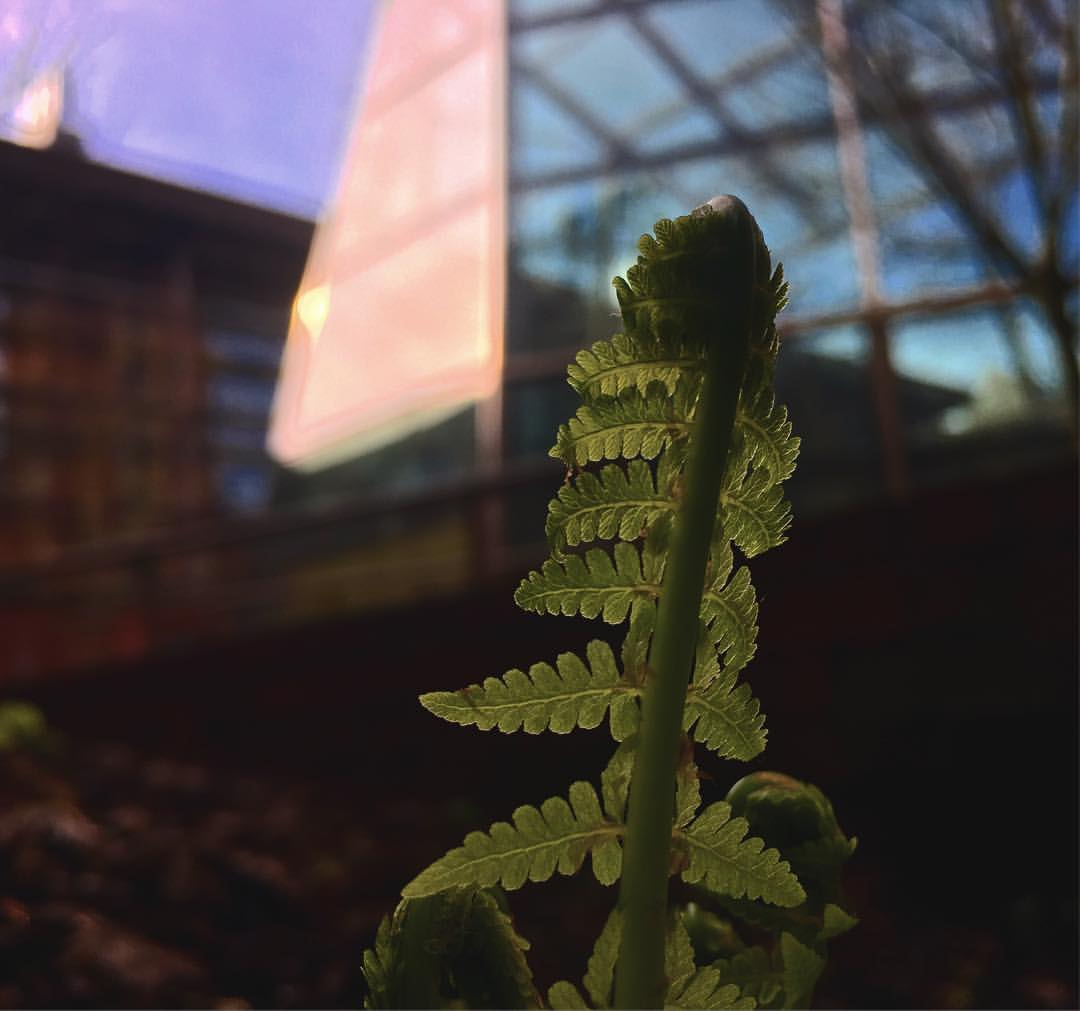
\includegraphics[width=\textwidth,trim={7cm 0 8cm 0},clip]{img/oppfern}
\end{center}
\end{column}
\end{columns}
\end{frame}

\begin{frame}{Closing Thoughts: Practical Applications}
\begin{figure}
  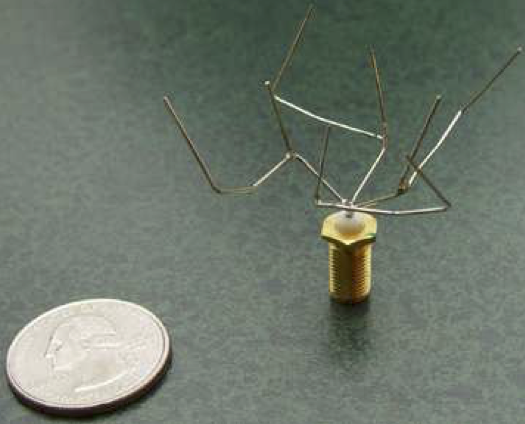
\includegraphics[width=0.7\textwidth]{img/evolved_antenna} 
  \hspace{2ex}
  \caption{A spacecraft antenna design generated using evolutionary methods \cite[Figure 2(a)]{Hornby2006AutomatedAlgorithms}.}
  \label{fig:evolved_antenna}
\end{figure}
\end{frame}

\begin{frame}{Closign Thoughts: Scientific Questions}
\begin{columns}
\begin{column}{0.6\textwidth}
\begin{itemize}
\item at what level of abstraction can the power of biological evolution be harnessed in a computational model?
\item what are the fundamental mechanisms at play in evolution?
\end{itemize}
\end{column}
\begin{column}{0.4\textwidth}
\begin{center}
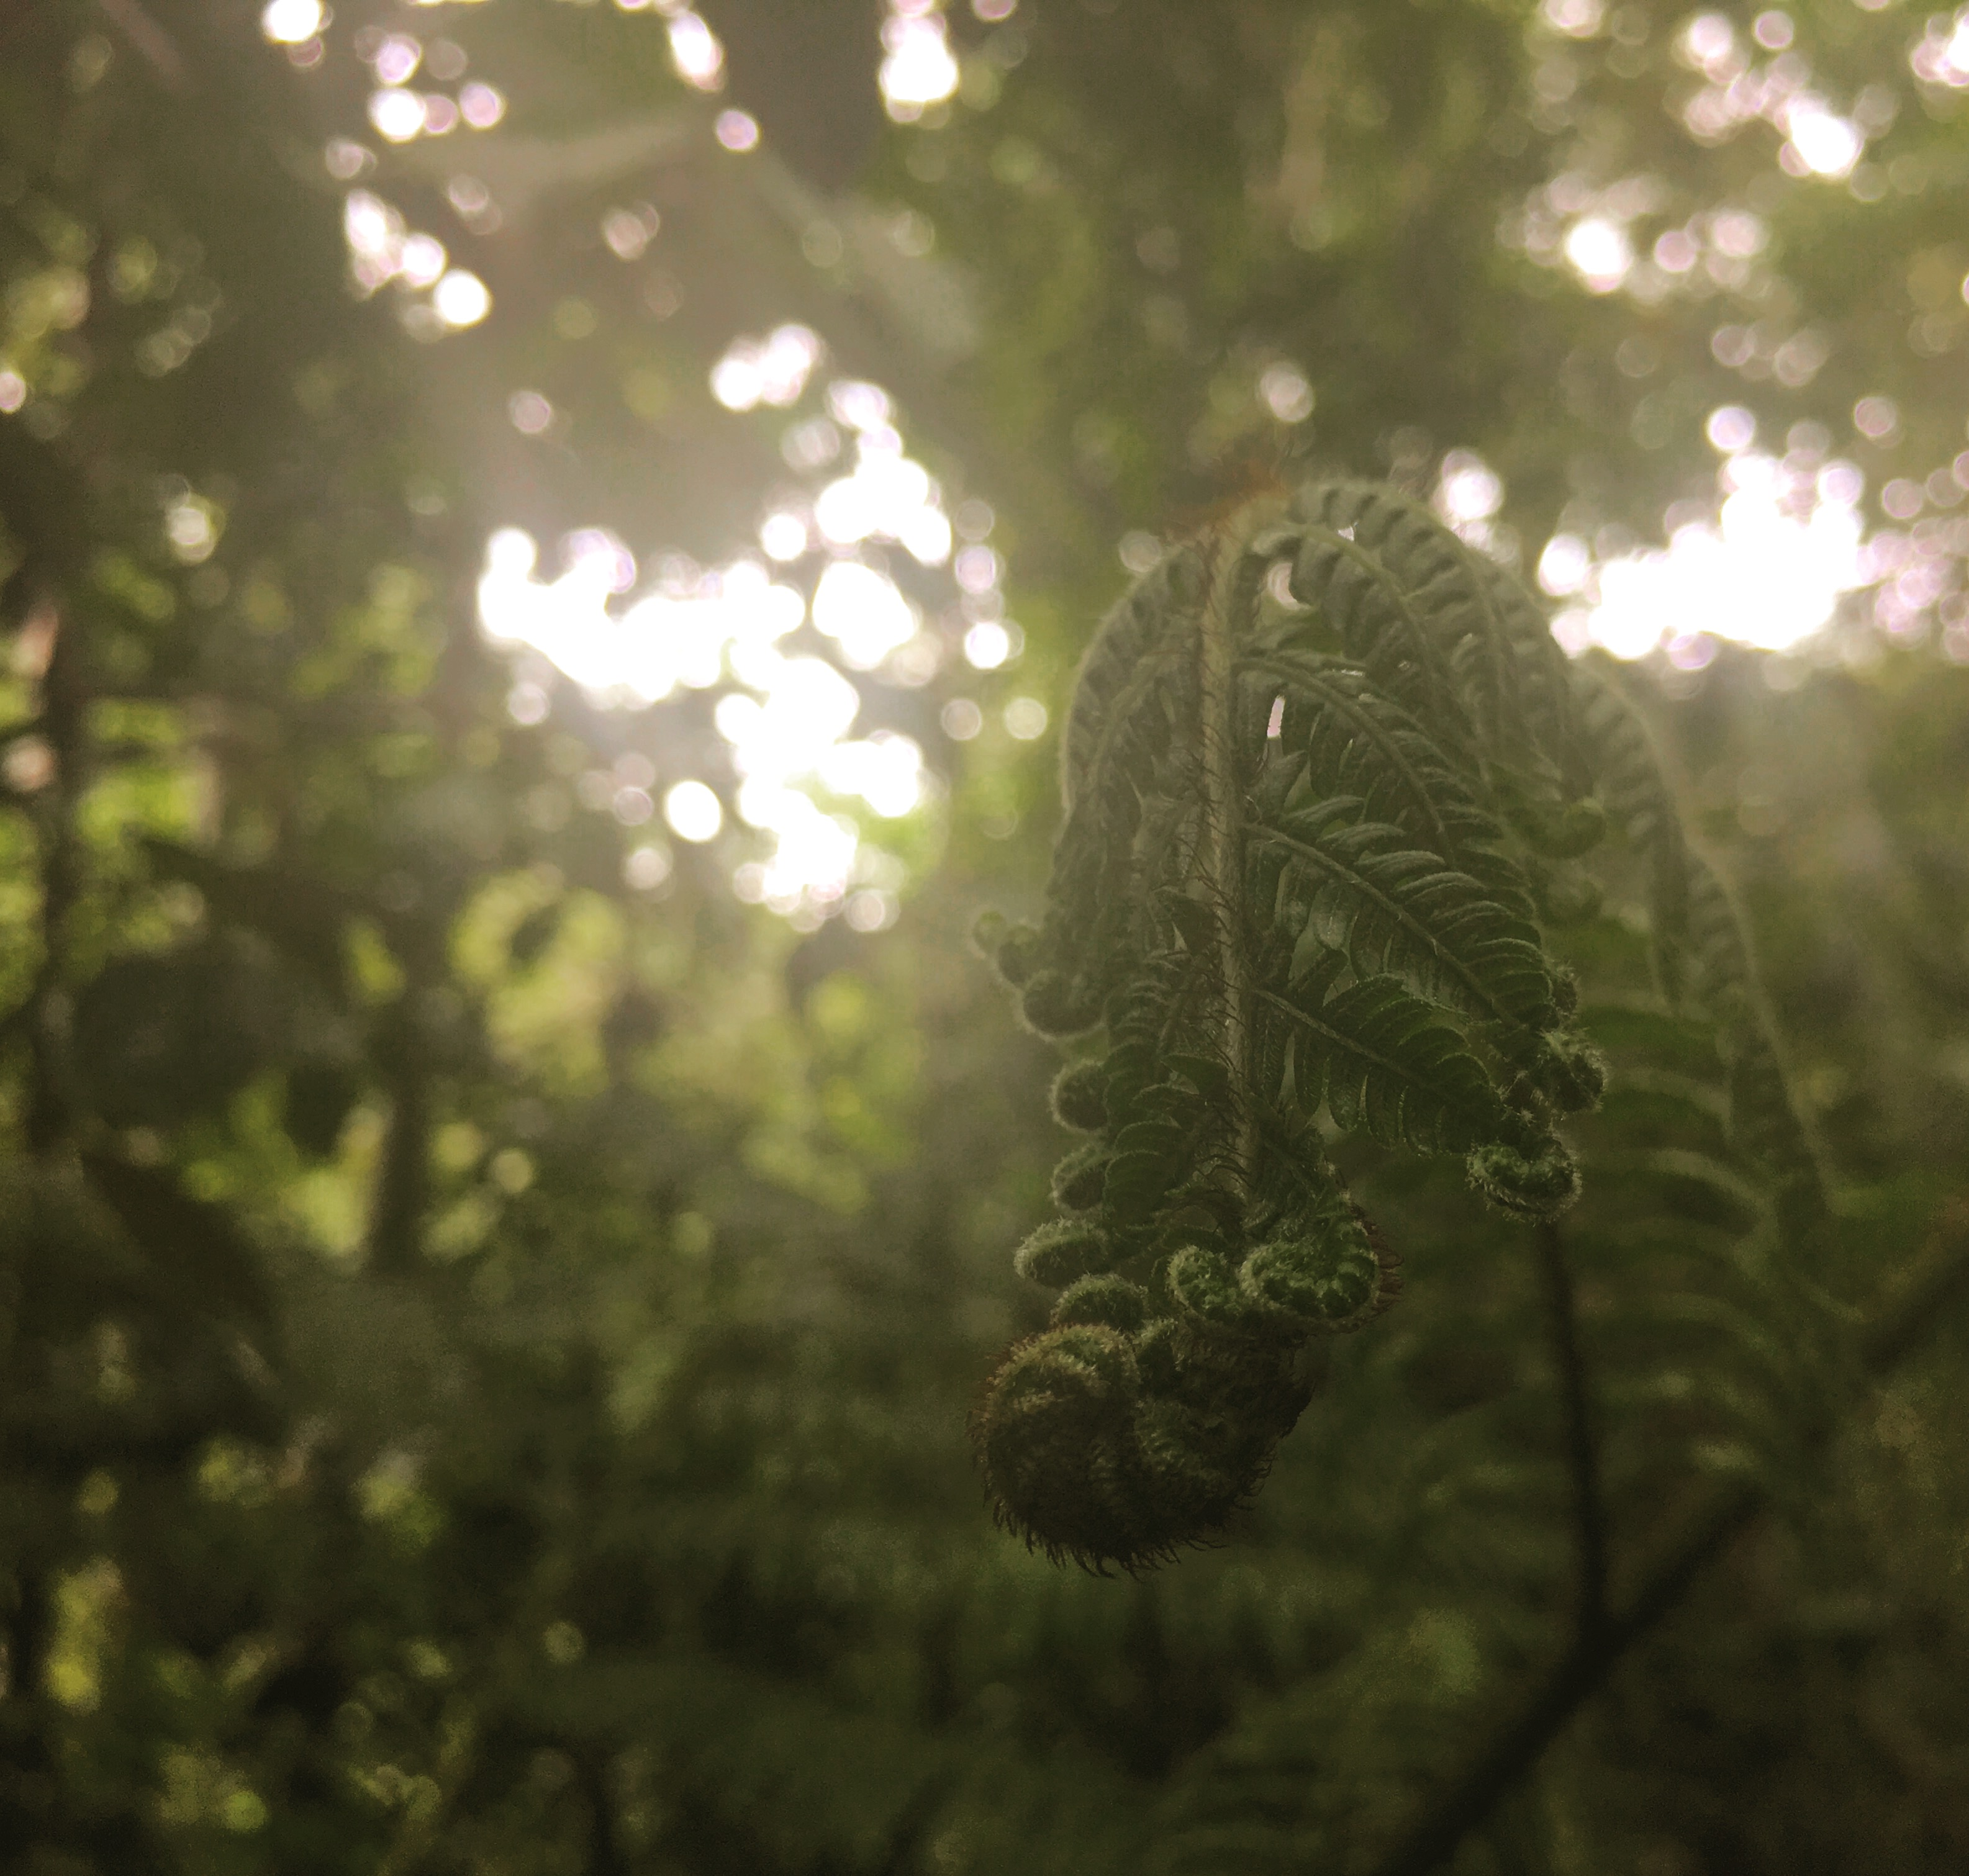
\includegraphics[width=\textwidth,trim={18cm 0 27cm 0},clip]{img/tropical_fern}
\end{center}
\end{column}
\end{columns}
\end{frame}

\begin{frame}{Closing Thoughts: Scientific Questions}
\begin{columns}
\begin{column}{0.6\textwidth}
\begin{itemize}
\item evolutionary biology provides continuing inspiration for new techniques in evolutionary computing
\item evolutionary models move theory evaluation from a qualitative endeavor towards a quantitative endeavor
\end{itemize}
\end{column}
\begin{column}{0.4\textwidth}
\begin{center}
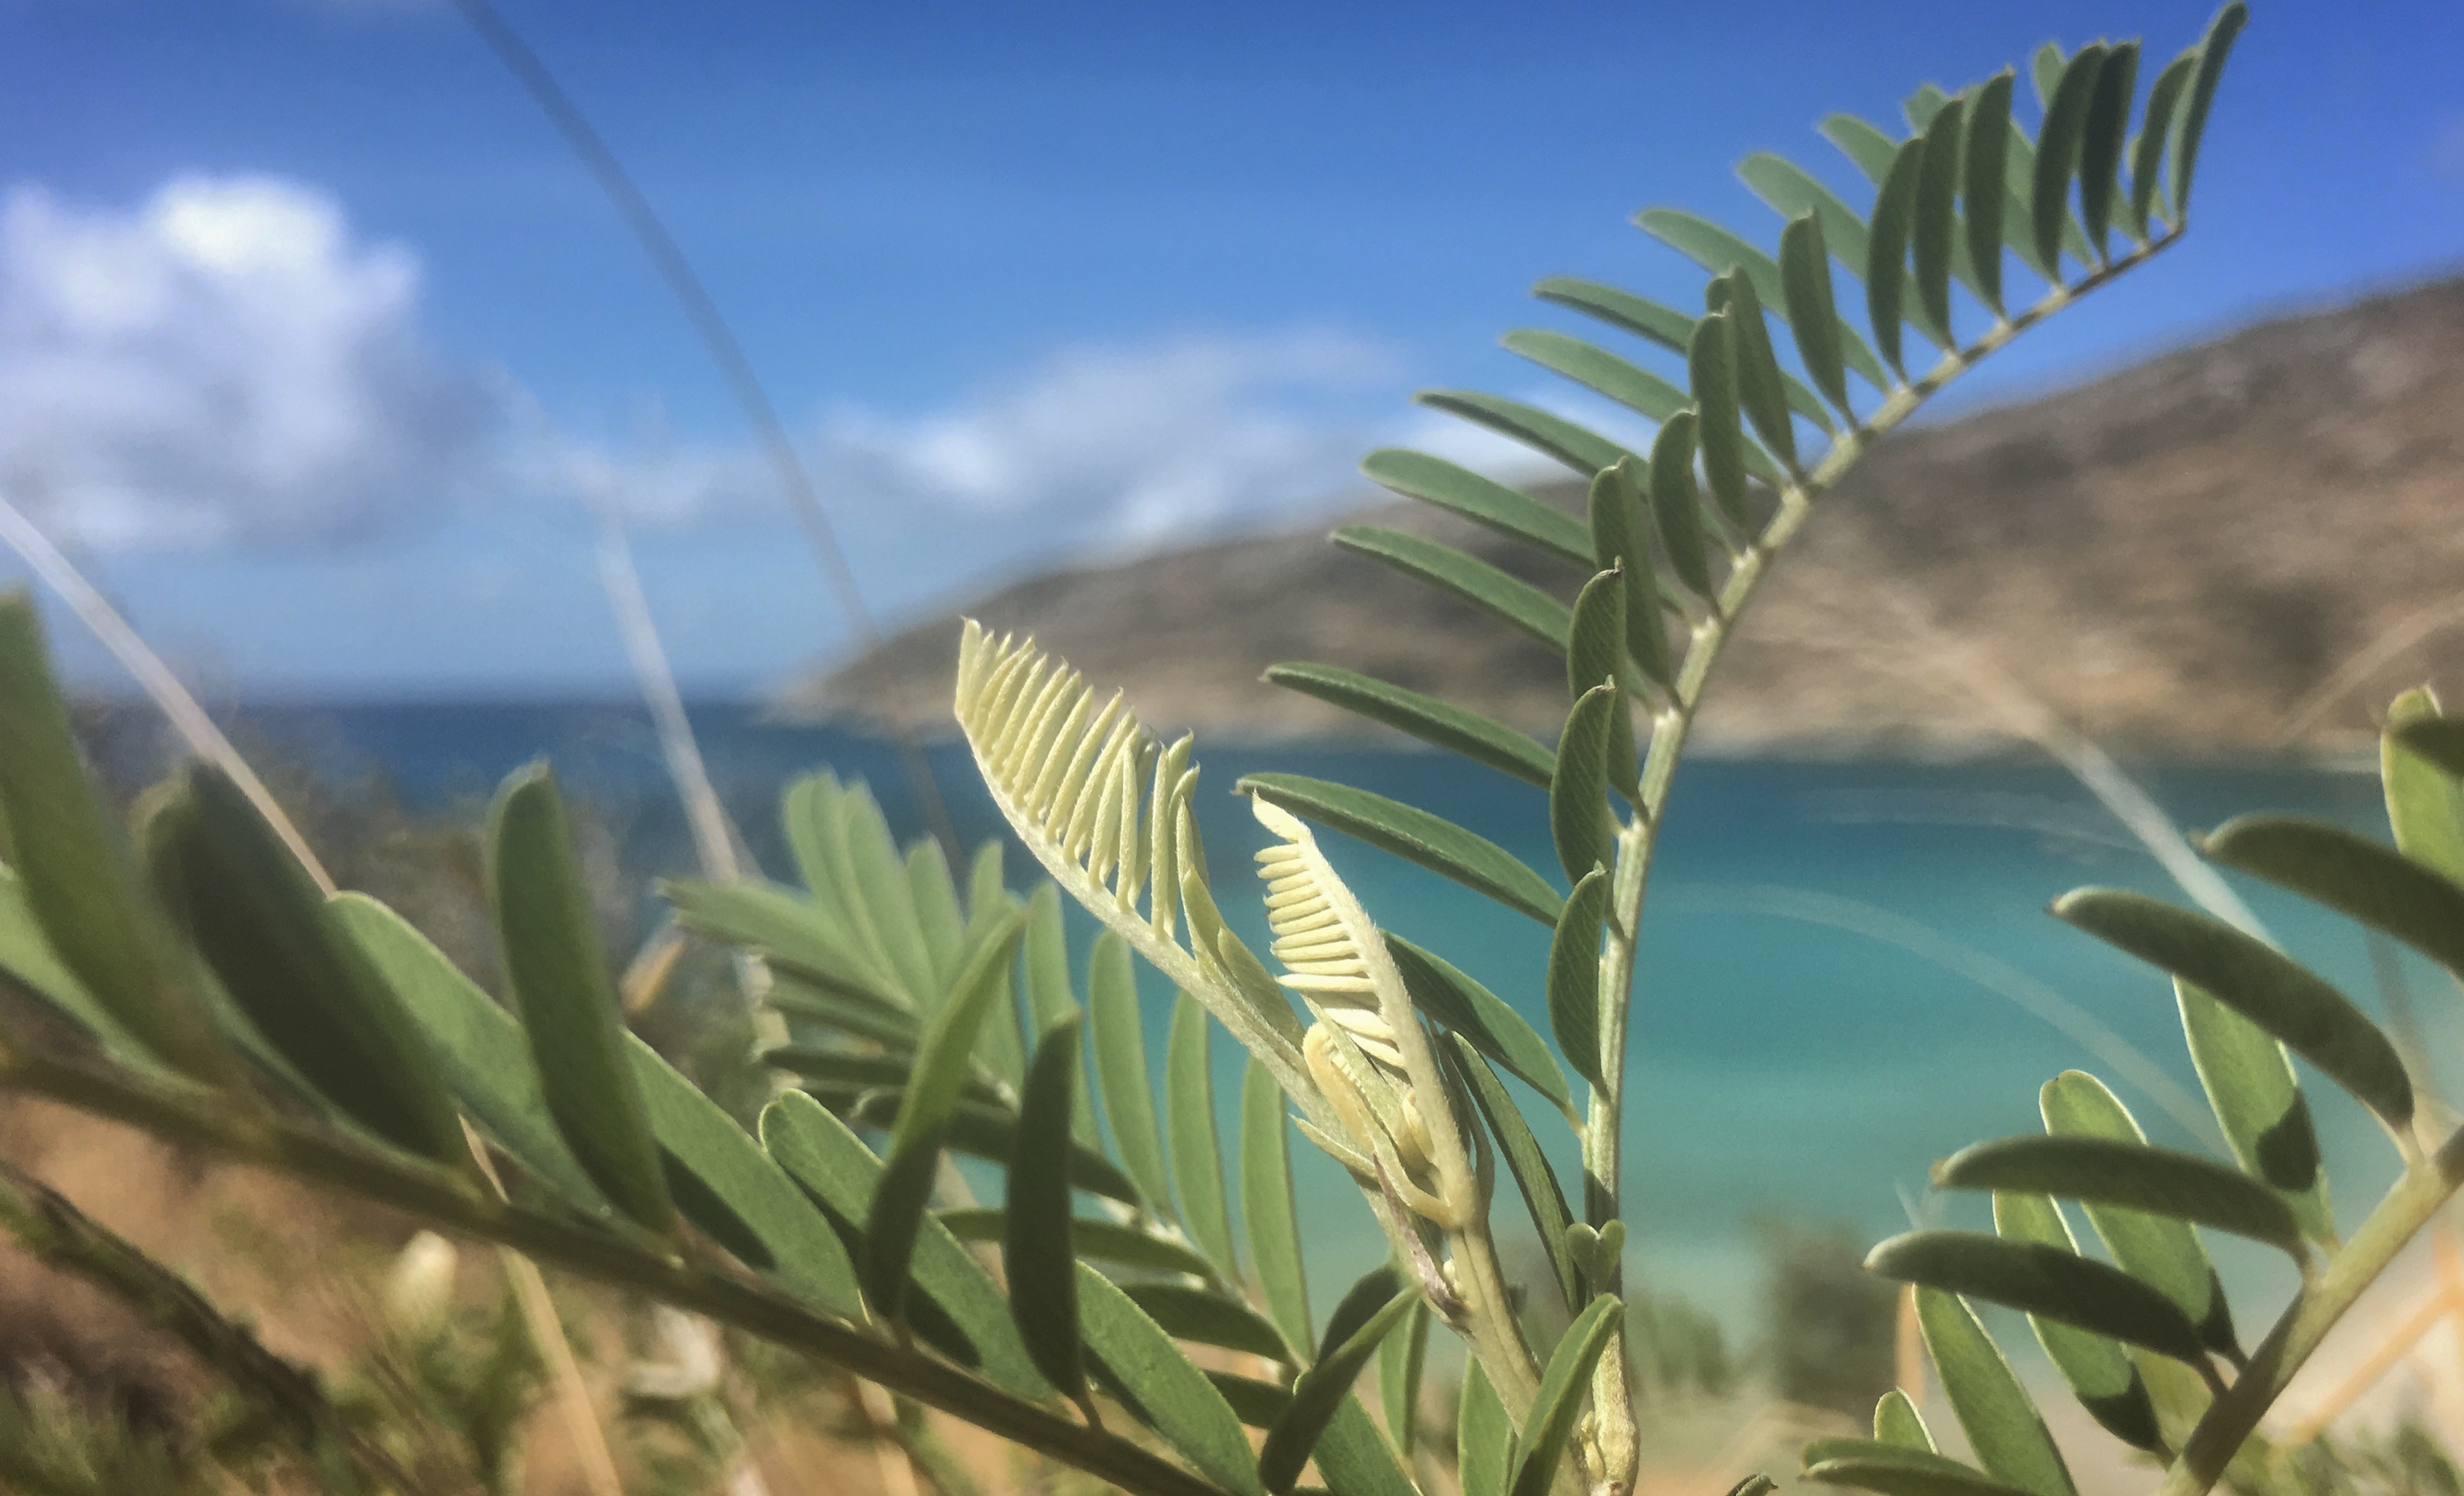
\includegraphics[width=\textwidth,trim={43cm 0 47cm 0},clip]{img/island_fern}
\end{center}
\end{column}
\end{columns}
\end{frame}

% \begin{frame}{Scientific Questions}
% \begin{displayquote}
% ``Many evolutionary biologists do not see a need to connect somatic adaptability to the generation of variation, and some see a need to keep them separate. For them, it is sufficient to say that random mutation is required and that the phenotypic variation arises haphazardly from it as random damage; the organism's current phenotype does not matter for the variation produced, and the output of variation is nearly random \cite[p 219]{Kirschner2005TheDilemma}.''
% \end{displayquote}
% \end{frame}

\appendix

\begin{frame}{Acknowledgements}
\begin{columns}
\begin{column}{0.6\textwidth}
\begin{itemize}
\item DEAP \cite{Fortin2012DEAP:Easy}
\item Professor Richards for leading CS capstone
\item Professor Chiu and Chili Johnson for lending me compute time
\item Professor Smith for serving as a thesis reader
\item Professor Chambers for serving as my thesis advisor
\end{itemize}
	\vspace{-1ex}
	\begin{center}{
    
\includegraphics[width= 0.3\textwidth]{img/UofPS_stacked_maroonRGB_PNG}}
    \end{center}

\end{column}
\begin{column}{0.4\textwidth}
\begin{center}
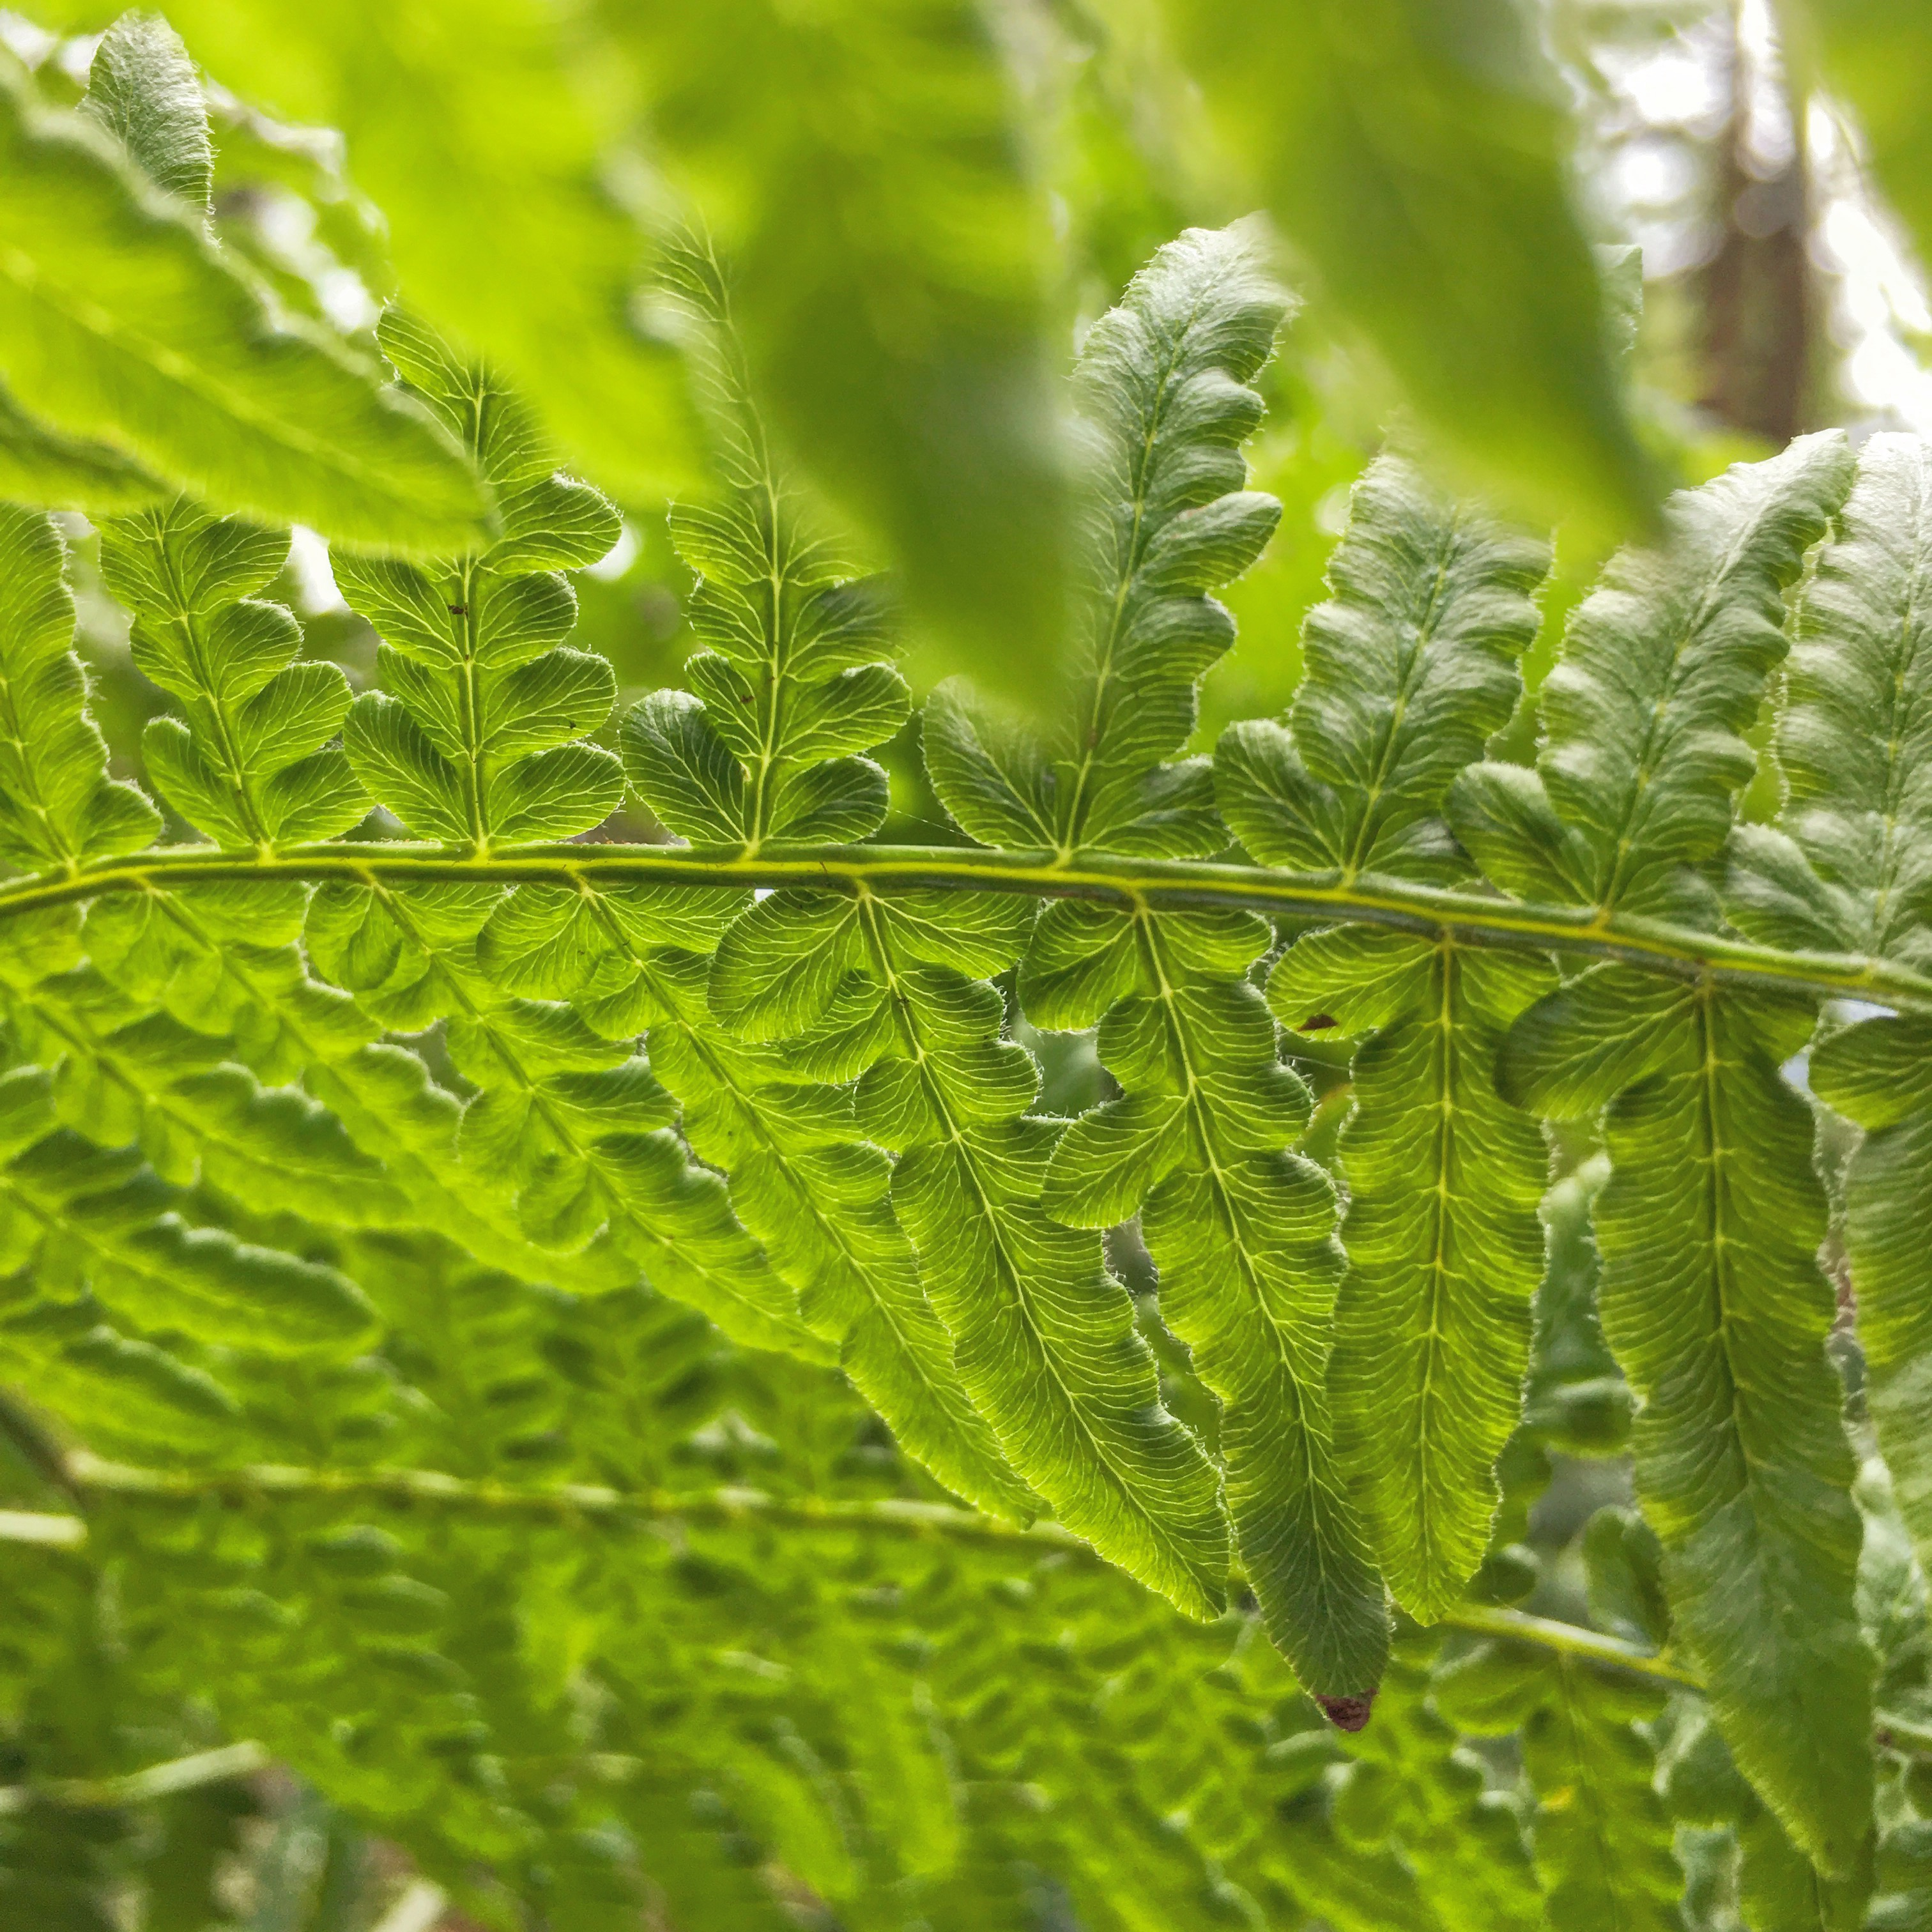
\includegraphics[width=\textwidth,trim={16cm 0 21cm 0},clip]{img/forest_fern}
\end{center}
\end{column}
\end{columns}

\end{frame}

\begin{frame}[standout]
  Questions?
\end{frame}

\begin{frame}[allowframebreaks]{References}

  \bibliography{Mendeley}
  \setbeamertemplate{bibliography item}{\insertbiblabel}
  %\nocite{*} % Insert publications even if they are not cited in the poster
  \bibliographystyle{apalike}
\end{frame}


\begin{frame}{Complete Model}
\begin{figure}
    \centering
    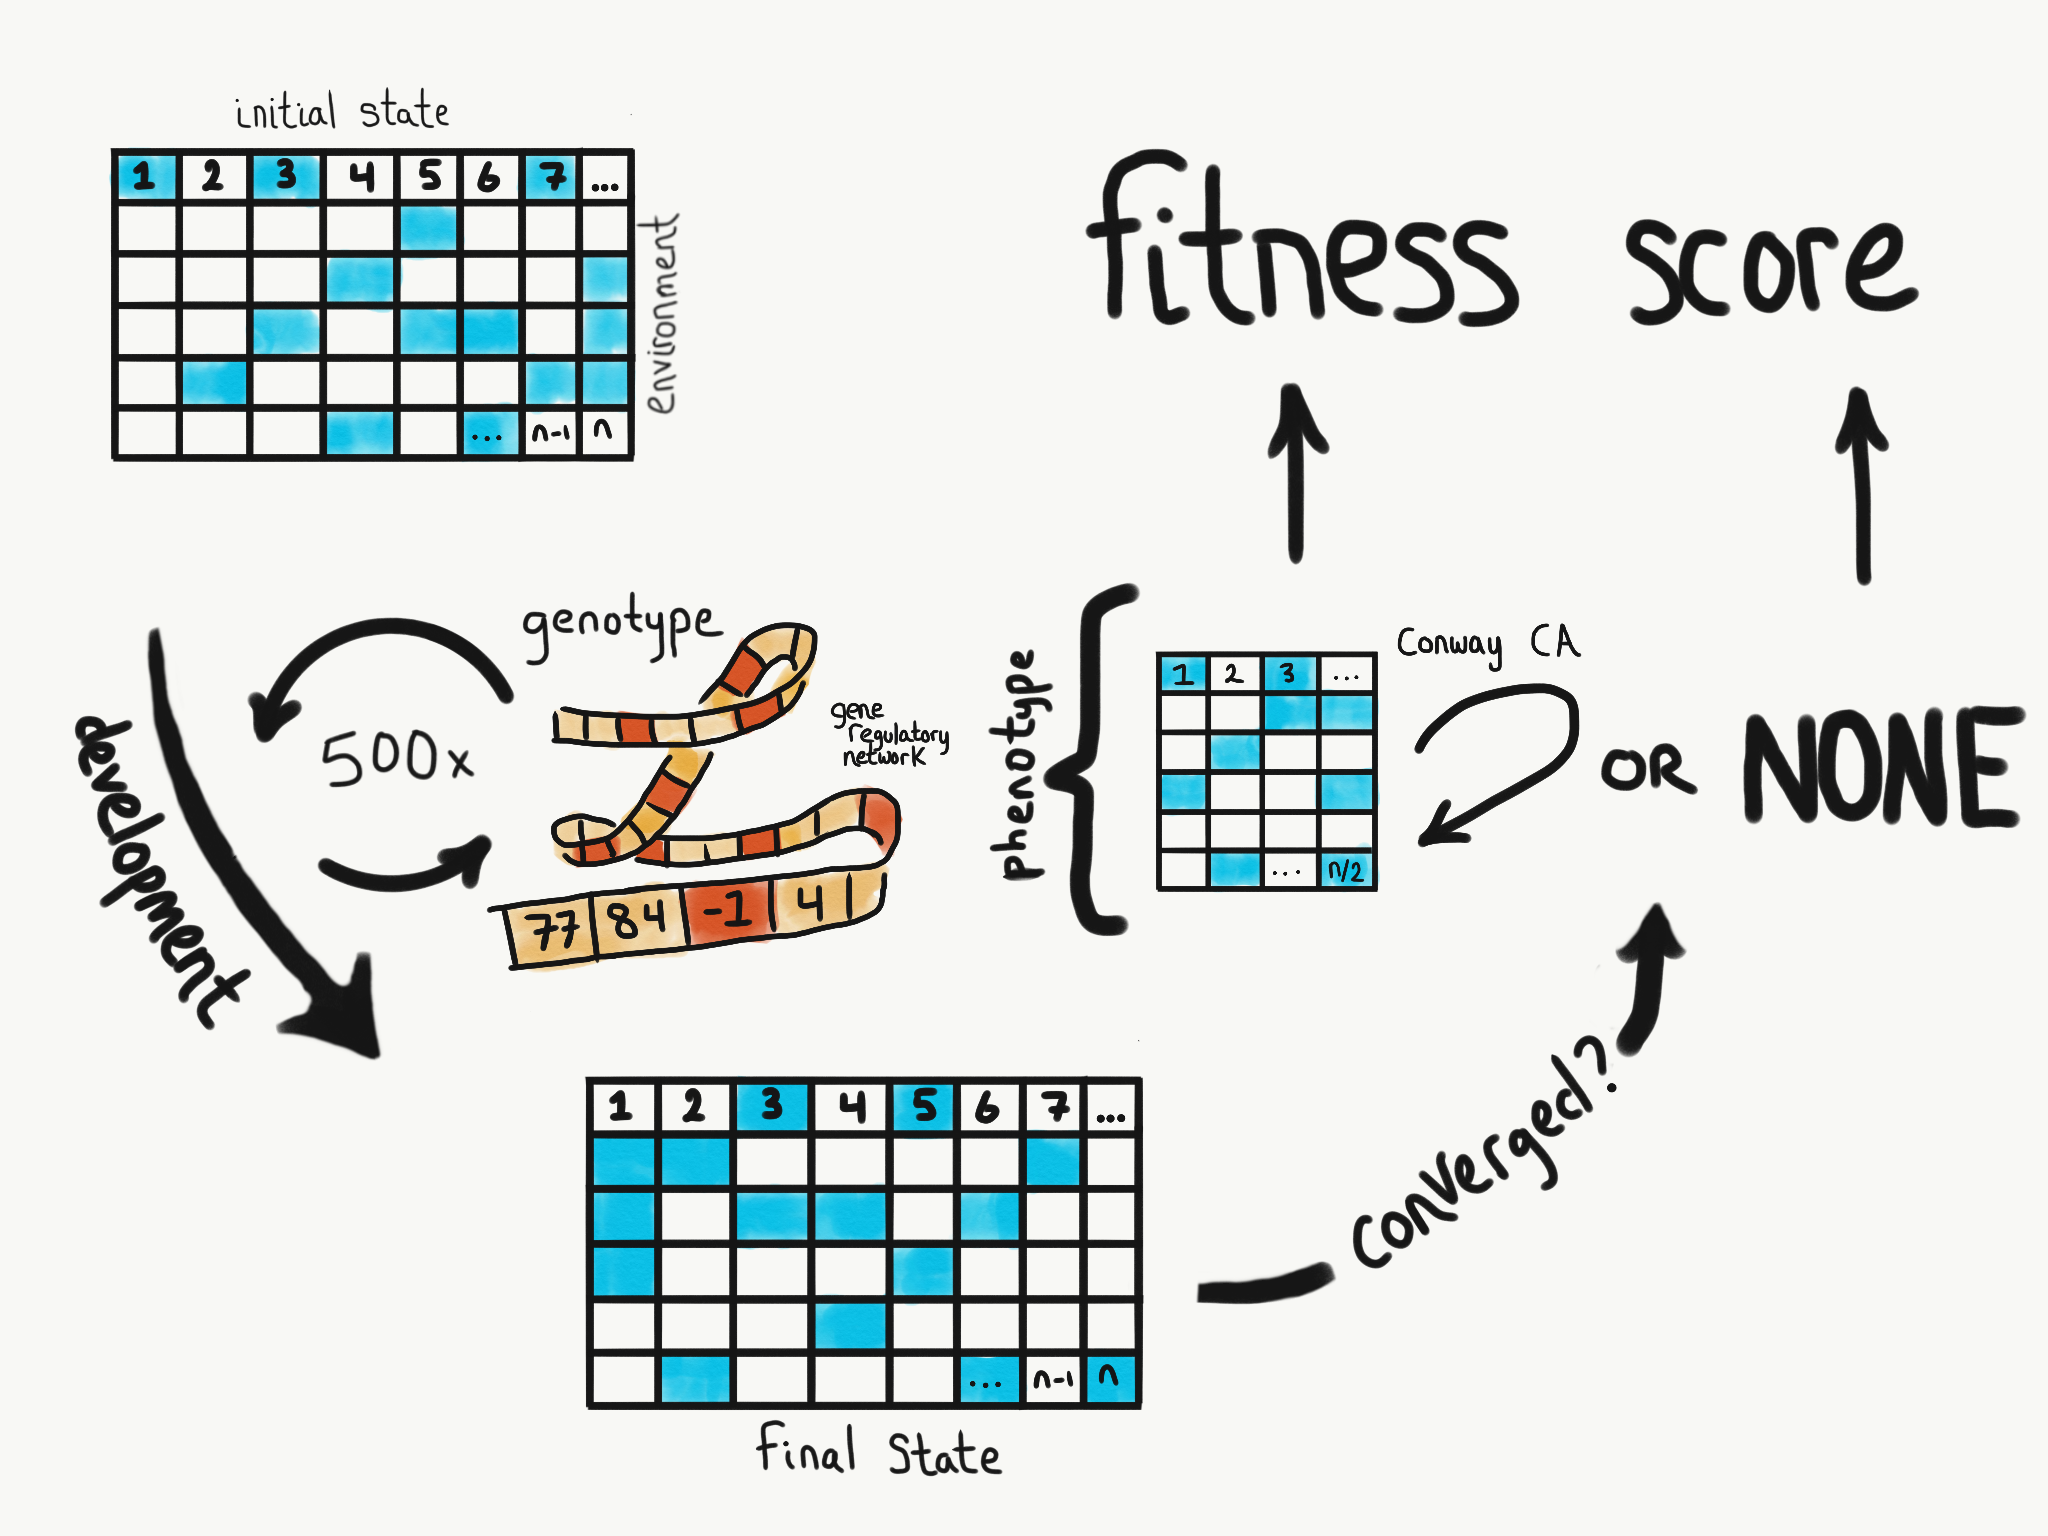
\includegraphics[width=0.8\textwidth]{img/complete_schematic}
 	\captionsetup{singlelinecheck=off,justification=raggedright}
  	\caption{A cartoon overview of the development and assessment processes of the expanded model, based loosely on \cite{Wilder2015ReconcilingEvolvability}.}
    \label{fig:complete_schematic}
\end{figure}
\end{frame}

\begin{frame}{Conway's Game of Life}
\begin{figure}
  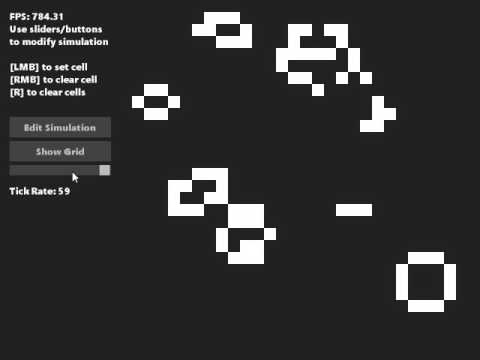
\includegraphics[width=0.8\textwidth]{img/gol_icon}
  \captionsetup{singlelinecheck=off,justification=raggedright}
\href{https://www.youtube.com/watch?v=Kzg5is1lgSk}{\caption{Video illustrations of Conway's Game of Life cellular automata in action.}}
\end{figure}
\end{frame}

\begin{frame}{Evidence for Indirect Plasticity}
\begin{figure}
    \centering
    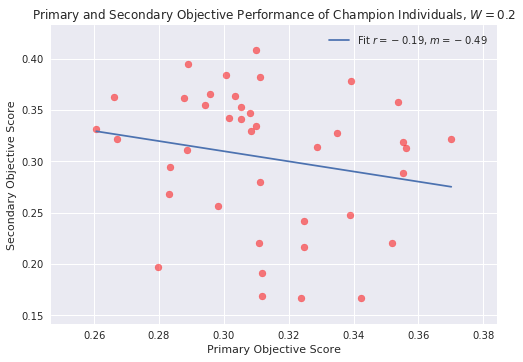
\includegraphics[width=0.8\textwidth]{img/primary_secondary_w02}
 	\captionsetup{singlelinecheck=off,justification=raggedright}
  	\caption{Primary and secondary objective performance of champion individuals evolved with primary and secondary condition/objective pair.}
    \label{fig:ev_w0}
\end{figure}
\end{frame}

\begin{frame}{Evidence for Indirect Plasticity}
\begin{figure}
    \centering
    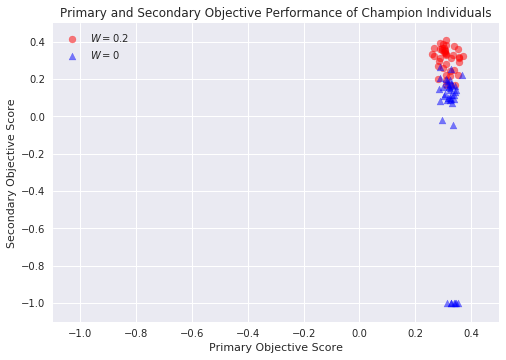
\includegraphics[width=0.8\textwidth]{img/scatter_indirect}
 	\captionsetup{singlelinecheck=off,justification=raggedright}
  	\caption{Comparison of objective performances of champions evolved with only primary condition/objective pair versus with both primary and secondary condition/objective pairs.}
    \label{fig:es_p0}
\end{figure}
\end{frame}

\begin{frame}{Evolvability as Novel Variation}
  \begin{figure}
 \centering
    \begin{subfigure}[b]{0.5\textwidth}
        \centering
    	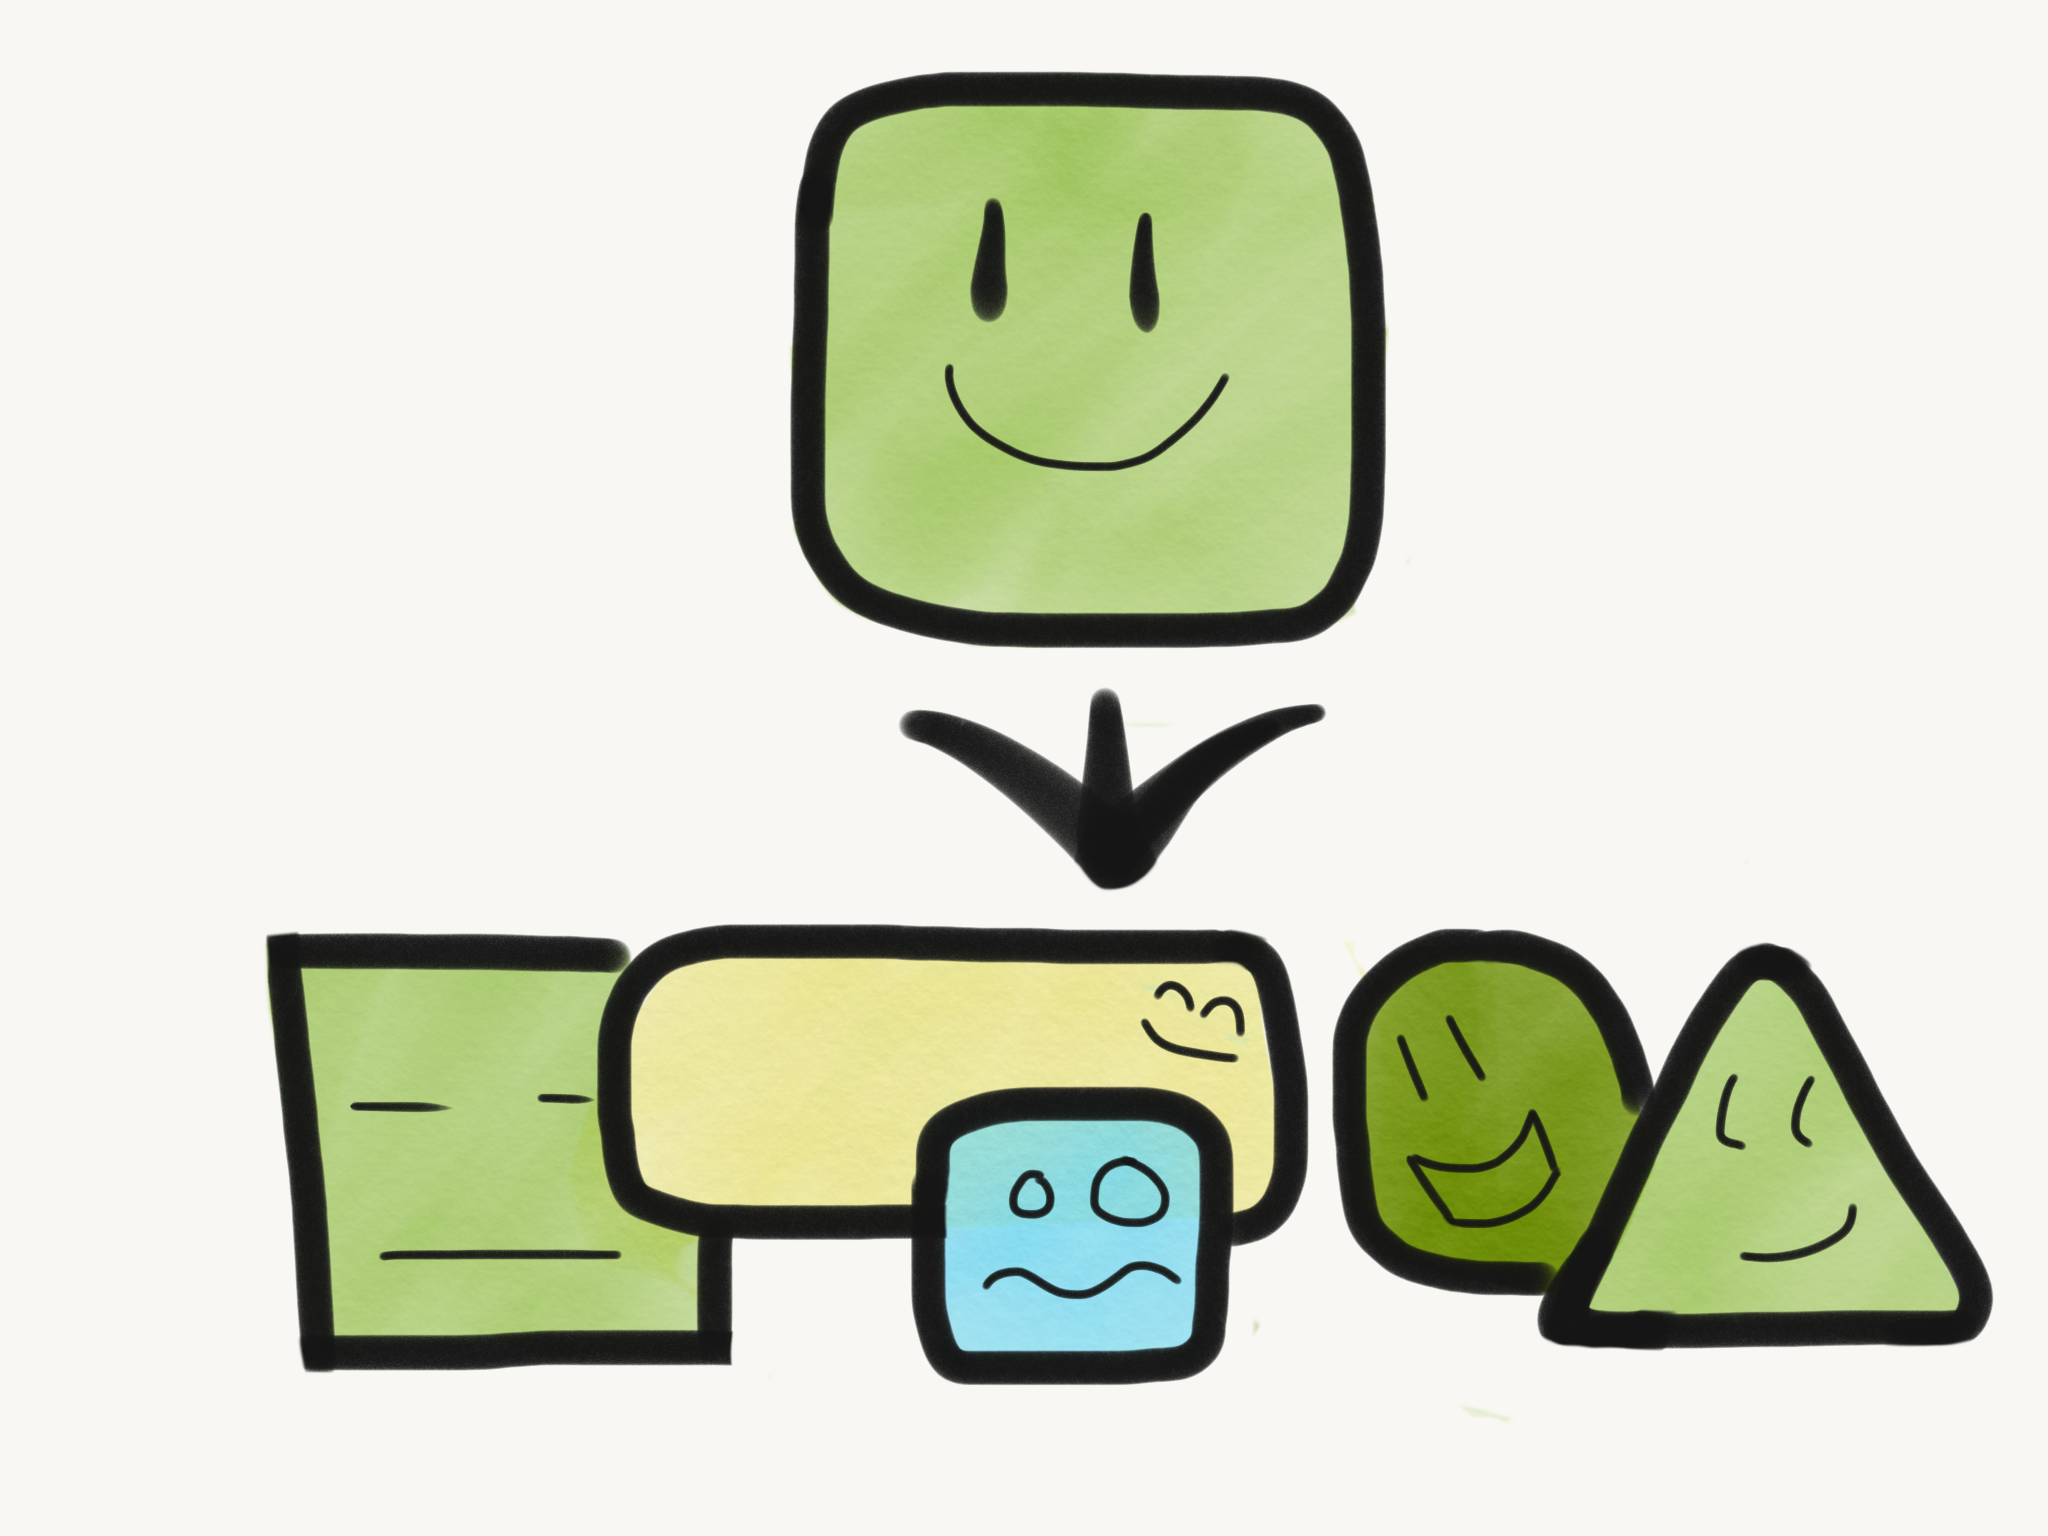
\includegraphics[width=\textwidth]{img/individual_evolvability}
        \caption{individual evolvability}
        \label{subfig:individual_evolvability}
    \end{subfigure}%
    \hfill
    \begin{subfigure}[b]{0.5\textwidth}
        \centering
        \includegraphics[width=\textwidth]{img/population_evolvability}
        \caption{population evolvability}
        \label{subfig:population_evolvability}
    \end{subfigure}
 	\captionsetup{singlelinecheck=off,justification=raggedright}
    \vspace{-4ex}
  \captionsetup{singlelinecheck=off,justification=raggedright}
  \caption{An illustration contrasting individual and population evolvability \cite{Wilder2015ReconcilingEvolvability}.}
  \label{fig:individual_vs_population_evolvability}
\end{figure}
\end{frame}

\begin{frame}{Promoting Evolvability: Fitness Niches}
	\begin{figure}
\begin{center}
\label{fig:cppn_images}
  \includegraphics[width=0.4\textwidth]{img/parent} \\
  \includegraphics[width=0.4\textwidth]{img/offspring} \\
  \includegraphics[width=0.4\textwidth]{img/better_goast}
  \end{center}
  \captionsetup{singlelinecheck=off,justification=raggedright}

  \caption{Illustration of compositional pattern producing networks (right) and their output images (left) generated via \cite{Ha2015Neurogram}.}
\end{figure}
\end{frame}

\begin{frame}{Promoting Evolvability: Fitness Niches}
\vfill
	\begin{figure} \label{fig:dnn}
  \begin{center}
  \includegraphics[width=0.5\textwidth]{img/recognize} \\
  \includegraphics[width=0.5\textwidth]{img/confused}
  \end{center}
  \captionsetup{singlelinecheck=off,justification=raggedright}

  \caption{A deep neural network (DNN) is trained to recognize a specific category of images.}
\end{figure}
    \vfill
\end{frame}

\begin{frame}{Promoting Evolvability: Fitness Niches}
\vspace{2ex}
	\begin{figure}
    \centering
  \begin{columns}
  \begin{column}{0.6\textwidth}
  \includegraphics[width=0.9\textwidth]{img/dnn_collection}
   \end{column}
   \begin{column}{0.4\textwidth}
   \includegraphics[width=0.9\textwidth]{img/cat}
   \end{column}
	\end{columns}
\captionsetup{singlelinecheck=off,justification=raggedright}
  	\caption{Several hundred fitness niches are defined using DNNs each trained to recognize different categories \cite{Nguyen2015InnovationLearning}.}
    \label{fig:niches}
\end{figure}
\end{frame}

\begin{frame}{Promoting Evolvability: Fitness Niches}
\vspace{2ex}	
\begin{figure}
    \centering
    \begin{columns}
    \begin{column}{0.7\textwidth}
     \includegraphics[width=\textwidth]{img/ie_phylogenetic_tree_combined}
    \end{column}
    \begin{column}{0.3\textwidth}
   	\captionsetup{singlelinecheck=off,justification=raggedright}
  	\caption{An illustration of goal-switching, where offspring from a parent that occupies one niche invade another \cite[Figure 9]{Nguyen2015InnovationLearning}. Individuals that promote phenotypically variable offspring are rewarded \cite{Mengistu2016EvolvabilityIt}.}
    \label{fig:goal_switching}
    \end{column}
    \end{columns}
   

\end{figure}
\end{frame}

\begin{frame}{Promoting Evolvability: Fitness Niches}
	\begin{figure}
    \centering
    \includegraphics[width=0.9\textwidth]{img/ie_greatest_hits}
 	\captionsetup{singlelinecheck=off,justification=raggedright}
  	\caption{Selected champion individuals from a sample of environmental niches \cite[Figure 7]{Nguyen2015InnovationLearning}.}
    \label{fig:ie_results}
\end{figure}
\end{frame}


\end{document}
